% ------------------------------------------------------------------------------
% The OpenQuake-engine Users Manual
%
% Authors:
% 	Marco Pagani 		- GEM Foundation, Pavia, Italy
% 	Vitor Silva 		- GEM Foundation, Pavia, Italy
%	Graeme Weatherill - GEM Foundation, Pavia, Italy
%  Anirudh Rao       - GEM Foundation, Pavia, Italy
%  Michele Simionato - GEM Foundation, Pavia, Italy
%
% Authors on previous versions:
%  Helen Crowley     - GEM Foundation, Pavia, Italy
%  Damiano Monelli   - GEM Foundation, Pavia, Italy
%
% License:
% Document distributed under the CC BY-NC-SA 4.0 License
% Creative Commons Attribution-NonCommercial-ShareAlike 4.0 International
% http://creativecommons.org/licenses/by-nc-sa/4.0/
%
% Copyright:
% © GEM Foundation, Pavia, Italy. 2013--2016.
% ------------------------------------------------------------------------------

%-------------------------------------------------------------------------------
%  PACKAGES AND OTHER DOCUMENT CONFIGURATIONS
%-------------------------------------------------------------------------------

\documentclass[11pt,fleqn]{book} % ------------------ Left-justified equations -
%%%%%%%%%%%%%%%%%%%%%%%%%%%%%%%%%%%%%%%%%%%%%%%%%%%%%%%%%%%%%%%%%%%%%%%%%%%%%%%%
% The GEM Technical Documentation LaTeX Template
% Version 1.0 (10/10/2015)
%
% Original author:
% Mathias Legrand (legrand.mathias@gmail.com)
%
% Adapted for use by the GEM Foundation by:
% James Brown (james.brown@globalquakemodel.org)
% Anirudh Rao (anirudh.rao@globalquakemodel.org)
%
% License:
% CC BY-NC-SA 3.0 (http://creativecommons.org/licenses/by-nc-sa/3.0/)
%
% Compiling this template:
% This template uses bibtex for its bibliography and makeindex for its index.
% When you first open the template, compile it from the command line with the
% commands below:
%
% 1) pdflatex -interaction=nonstopmode oq-manual.tex
% 2) bibtex oq-manual
% 3) pdflatex -interaction=nonstopmode oq-manual.tex
% 4) pdflatex -interaction=nonstopmode oq-manual.tex
% 5) makeindex oq-manual.idx
% 6) makeglossaries oq-manual
% 7) pdflatex -interaction=nonstopmode oq-manual.tex
%
% After this, when you wish to update the bibliography/index use the appropriate
% command above and make sure to compile with pdflatex several times
% afterwards to propagate your changes to the document.
%
% This template also uses a number of packages which may need to be updated
% to the newest versions for the template to compile. It is strongly
% recommended you update your LaTeX distribution if you have any
% compilation errors.
%
% Important note:
% Chapter heading images should have a 2:1 width:height ratio,
% e.g. 920px width and 460px height.
%
%%%%%%%%%%%%%%%%%%%%%%%%%%%%%%%%%%%%%%%%%%%%%%%%%%%%%%%%%%%%%%%%%%%%%%%%%%%%%%%%

%-------------------------------------------------------------------------------
%  PACKAGES AND OTHER DOCUMENT CONFIGURATION
%-------------------------------------------------------------------------------

% Page layout and margins
\usepackage[top=3cm,bottom=3cm,left=3.2cm,right=3.2cm,headsep=10pt,a4paper]{geometry}
\linespread{1.25}

% Font settings
\usepackage[condensed]{roboto} % Use the Roboto font for headings
\usepackage[bitstream-charter]{mathdesign} % Use the Bitstream Charter font for text
% \usepackage{amsmath,amsfonts,amssymb,amsthm} % For math equations, theorems, symbols, etc
\usepackage{microtype} % Slightly tweak font spacing for aesthetics
\usepackage[utf8]{inputenc} % Required for including letters with accents
\usepackage[T1]{fontenc} % Use 8-bit encoding that has 256 glyphs

% Color settings
\usepackage{color, colortbl}
\usepackage{xcolor} % Required for specifying colors by name
\definecolor{darkgray}{gray}{.25}
\definecolor{lightgray}{gray}{.98}
% Colors from the GEM Brand Guidelines
\definecolor{oqblue}{RGB}{27,117,165}
\definecolor{gembrown}{cmyk}{.53,.54,.55,.54}

% Bibliography settings
\usepackage{csquotes}
\usepackage[style=alphabetic,
            sorting=nyt,
            sortcites=true,
            natbib=true,
            style=authoryear,
            maxcitenames=2,
            maxbibnames=100,
            autopunct=true,
            autolang=hyphen,
            hyperref=true,
            doi=true,
            abbreviate=false,
            backref=true,
            backend=bibtex,
            bibencoding=ascii,
            firstinits=true,
	    	uniquename=false,
	    	uniquelist=false]{biblatex}
\addbibresource{bibliography/hazard.bib} % Hazard BibTeX bibliography file
\addbibresource{bibliography/risk.bib} % Risk BibTeX bibliography file
\defbibheading{bibempty}{}

% Figure caption settings
\usepackage[textfont=it,margin=10pt,font=small,labelfont=bf,labelsep=endash]{caption}
\usepackage{subcaption}

% Rotate any object
\usepackage{rotating}

% Verbatim environments
\usepackage{verbatim}
\usepackage{fancyvrb}

% Index settings
\usepackage{calc} % Infix notation for \setcounter, \addtocounter, \setlength, \addtolength
\usepackage{imakeidx} % Required to make an index
\setcounter{secnumdepth}{3}
\setcounter{tocdepth}{3} % Entries down to \subsubsections in the TOC
\makeindex[title=Index,columns=2,intoc] % Create the files required for indexing

\usepackage{todonotes}
\usepackage{marginnote}
% Bold symbols in maths mode
\usepackage{bm}

% Flexible typesetting of tables and figures
\usepackage{ctable}
\usepackage{booktabs}

% Customization of section titles and table of contents
\usepackage{titlesec}
\usepackage{titletoc}

% Header and footer customization
\usepackage{fancyhdr}
\usepackage{etoolbox}

\usepackage{graphicx} % Required for including pictures
\usepackage{tikz} % Required for drawing custom shapes
\usepackage{eso-pic} % Required for specifying an image background in the title page
\usepackage{pdfpages} % Needed to load .pdf pages, used for the cover page

% English language hyphenation
\usepackage[english]{babel}

\usepackage{enumitem} % Customize lists
\setlist{nolistsep} % Reduce spacing between bullet points and numbered lists
\usepackage{listings} % Required for embedding code snippets
\usepackage[cache=true]{minted} % Syntax highlighting for xml

\usepackage{hyperref}
\hypersetup{hidelinks,colorlinks=true,breaklinks=true,citecolor=oqblue,linkcolor=gembrown,urlcolor=oqblue,bookmarksopen=false,pdftitle={Title},pdfauthor={Author}}

% Package to create a glossary - must be loaded after hyperref
\usepackage[acronym,nonumberlist,style=altlist,section=section,toc]{glossaries}
\makeglossaries


%----------------------------------------------------------------------------------------
%     MAIN TABLE OF CONTENTS
%----------------------------------------------------------------------------------------

% Remove the default margin
\contentsmargin{0cm}

% \titlecontents{section}
%                       [left]
%                       {above}
%                       {before with label}
%                       {before without label}
%                       {filler and page}
%                       [after]

% Part text styling
\titlecontents{part}
                    [0cm] % Indentation
                    {\addvspace{24pt}\Large\sffamily\bfseries} % Spacing and font options for parts
                    {\color{black!60}\contentslabel[\Large\thecontentslabel]{1.25cm}\color{black}} % Part number
                    {}
                    {\color{black!60}\Large\sffamily\bfseries\hfill\thecontentspage} % Page number
                    []

% Chapter text styling
\titlecontents{chapter}
                    [1.25cm] % Indentation
                    {\addvspace{18pt}\large\sffamily\bfseries} % Spacing and font options for chapters
                    {\color{darkgray!80}\contentslabel[\Large\thecontentslabel]{1.25cm}\color{darkgray}} % Chapter number
                    {\color{darkgray}}
                    {\color{darkgray!40}\large\sffamily\bfseries\;\titlerule*[.5pc]{.}\;\color{darkgray!80}\thecontentspage} % Page number
                    []

% Section text styling
\titlecontents{section}
                    [1.25cm] % Indentation
                    {\addvspace{12pt}\sffamily\bfseries} % Spacing and font options for sections
                    {\color{black!60}\contentslabel[\thecontentslabel]{1.25cm}\color{black}} % Section number
                    {}
                    {\color{black!20}\normalsize\sffamily\bfseries\;\titlerule*[.5pc]{.}\;\color{black!60}\thecontentspage} % Page number
                    []

% Subsection text styling
\titlecontents{subsection}
                    [1.25cm] % Indentation
                    {\addvspace{6pt}\sffamily\small} % Spacing and font options for subsections
                    {\color{black!60}\contentslabel[\thecontentslabel]{1.25cm}\color{black}} % Subsection number
                    {}
                    {\color{black!20}\normalsize\sffamily\;\titlerule*[.5pc]{.}\;\color{black!60}\thecontentspage} % Page number
                    []

% Subsubsection text styling
\titlecontents{subsubsection}
                    [1.25cm] % Indentation
                    {\addvspace{3pt}\sffamily\footnotesize} % Spacing and font options for subsubsections
                    {\color{black!60}\contentslabel[\thecontentslabel]{1.25cm}\color{black}\em} % Subsubsection number
                    {}
                    {\color{black!20}\normalsize\sffamily\;\titlerule*[.5pc]{.}\;\color{black!60}\thecontentspage} % Page number
                    []

%----------------------------------------------------------------------------------------
%     MINI TABLE OF CONTENTS IN CHAPTER HEADS
%----------------------------------------------------------------------------------------

% Section text styling
\titlecontents{lsection}[0em] % Indendation
{\footnotesize\sffamily} % Font settings
{}
{}
{}

% Subsection text styling
\titlecontents{lsubsection}[.5em] % Indentation
{\normalfont\footnotesize\sffamily} % Font settings
{}
{}
{}

%----------------------------------------------------------------------------------------
%     PAGE HEADERS
%----------------------------------------------------------------------------------------

% Patch fancyhdr to set the font and rule colors for headers and footers
\makeatletter
\patchcmd{\@fancyhead}{\rlap}{\color{oqblue}\rlap}{}{}
\patchcmd{\headrule}{\hrule}{\color{black}\hrule}{}{}
\patchcmd{\@fancyfoot}{\rlap}{\color{oqblue}\rlap}{}{}
\patchcmd{\footrule}{\hrule}{\color{black}\hrule}{}{}
\makeatother

\pagestyle{fancy}
\renewcommand{\chaptermark}[1]{\markboth{\sffamily\normalsize\bfseries\chaptername\ \thechapter.\ #1}{}} % Chapter text font settings
\renewcommand{\sectionmark}[1]{\markright{\sffamily\normalsize\thesection\hspace{5pt}#1}{}} % Section text font settings
\fancyhf{} \fancyhead[LE,RO]{\sffamily\normalsize\thepage} % Font setting for the page number in the header
\fancyhead[LO]{\rightmark} % Print the nearest section name on the left side of odd pages
\fancyhead[RE]{\leftmark} % Print the current chapter name on the right side of even pages
\renewcommand{\headrulewidth}{0.5pt} % Width of the rule under the header
\addtolength{\headheight}{7.5pt} % Increase the spacing around the header
\renewcommand{\footrulewidth}{0pt} % Removes the rule in the footer
\fancypagestyle{plain}{\fancyhead{}\renewcommand{\headrulewidth}{0pt}} % Style for when a plain pagestyle is specified

% Remove the header from odd empty pages at the end of chapters
\makeatletter
\renewcommand{\cleardoublepage}{
\clearpage\ifodd\c@page\else
\hbox{}
\vspace*{\fill}
\thispagestyle{empty}
\newpage
\fi}
\makeatother

%----------------------------------------------------------------------------------------
%     SECTION NUMBERING IN THE MARGIN
%----------------------------------------------------------------------------------------

\makeatletter
\renewcommand{\@seccntformat}[1]{\llap{\textcolor{oqblue}{\csname the#1\endcsname}\hspace{1em}}}
\renewcommand{\section}{\@startsection{section}{1}{\z@}
{-4ex \@plus -1ex \@minus -.4ex}
{1ex \@plus.2ex }
{\normalfont\large\sffamily\bfseries}}
\renewcommand{\subsection}{\@startsection {subsection}{2}{\z@}
{-3ex \@plus -0.1ex \@minus -.4ex}
{0.5ex \@plus.2ex }
{\normalfont\sffamily\bfseries}}
\renewcommand{\subsubsection}{\@startsection {subsubsection}{3}{\z@}
{-2ex \@plus -0.1ex \@minus -.2ex}
{.2ex \@plus.2ex }
{\normalfont\small\sffamily\bfseries}}
\renewcommand{\paragraph}{\@startsection {paragraph}{4}{\z@}
{-2ex \@plus-.2ex \@minus .2ex}
{.1ex}
{\normalfont\small\sffamily\bfseries\em}}
\makeatother

%----------------------------------------------------------------------------------------
%     PART HEADINGS
%----------------------------------------------------------------------------------------

% \titleformat{command}[shape]{format}{label}{sep}{before}[after]
\titleformat{\part}[display]{\bfseries\filcenter\Huge\sffamily}{\textcolor{gembrown}{\partname~\thepart}}{20pt}{\textcolor{gembrown}}

%----------------------------------------------------------------------------------------
%     CHAPTER HEADINGS
%----------------------------------------------------------------------------------------

% The set-up below should be manually adapted to the overall page
% layout and margin setup controlled by the geometry package.

\newcommand{\thechapterimage}{}
\newcommand{\chapterimage}[1]{\renewcommand{\thechapterimage}{#1}}

% Numbered chapters with mini tableofcontents
\makeatletter
\def\thechapter{\arabic{chapter}}
\def\@makechapterhead#1{
\thispagestyle{empty}
{\centering \normalfont\sffamily
\ifnum \c@secnumdepth >\m@ne
\if@mainmatter
\startcontents
\begin{tikzpicture}[remember picture,overlay]
\node at (current page.north west)
{\begin{tikzpicture}[remember picture,overlay]
\node[anchor=north west,inner sep=0pt] at (0,0) {\includegraphics[width=\paperwidth]{\thechapterimage}};

% Commenting the 3 lines below removes the small contents box in the chapter heading
\fill[color=oqblue!10!white,opacity=.6] (1cm,0) rectangle (12cm,-7cm);
\node[anchor=north west] at (1.5cm,.05cm) {\parbox[t][6.9cm][t]{10.5cm}{
    \huge\bfseries\flushleft \printcontents{l}{1}{\setcounter{tocdepth}{2}}}};
% The 3 lines below control the box environment for chapter titles
\draw[anchor=west] (1.8cm,-10cm) node [fill=white,text opacity=1,draw=white,draw opacity=1,line width=1.5pt,fill opacity=.6,inner sep=12pt]{\huge\sffamily\bfseries\textcolor{oqblue}{\thechapter.\hspace{0.35cm}#1\strut\makebox[22cm]{}}};

\end{tikzpicture}};
\end{tikzpicture}}
\par\vspace*{230\p@}
\fi
\fi}

% Unnumbered chapters without mini tableofcontents
\def\@makeschapterhead#1{
\thispagestyle{empty}
{\centering \normalfont\sffamily
\ifnum \c@secnumdepth >\m@ne
\if@mainmatter
\begin{tikzpicture}[remember picture,overlay]
\node at (current page.north west)
{\begin{tikzpicture}[remember picture,overlay]
\draw[anchor=west] (2.6cm,-4.2cm) node [fill=white,text opacity=1,draw=white,draw opacity=1,line width=1.5pt,fill opacity=.6,inner sep=12pt]{\huge\sffamily\bfseries\textcolor{oqblue}{#1\strut\makebox[22cm]{}}};
\end{tikzpicture}};
\end{tikzpicture}}
\par\vspace*{40\p@}
\fi
\fi
}
\makeatother % ------------- Load packages and template -
\graphicspath{{figures/}} % -------------- Directory where pictures are stored -

\begin{document}
% OpenQuake Book Glossary
% To cite a glossary element in a document:
%\gls{seismicsourcedata}
%\Gls{seismicsourcedata} - First initial is uppercase
%\GLS{seismicsourcedata} - All initials are uppercase
%\glspl{seismicsourcedata} - Plural
% To process the glossary:
% makeglossaries oq-manual


% ------- A

\newglossaryentry{areasource}{
	name=area source,
	description={A source type usually adopted to model distributed
	seismicity. In an area source the seismicity occurrence rate is assumed
	uniform over the source area; this produces an hazard pattern with a
	plateau of constant hazard inside the polygon delimiting the area source
	and values of hazard that tend to decrease as we move away from the
	border of the source}
}


\newglossaryentry{asset}{
	name=asset,
	description={An asset is an element with a certain value, which can include
	buildings or population. For example, an asset can include an individual
	building at a given location, or a number of buildings that are grouped, co-
	located at a single location and classified with the same \gls{taxonomy}}
}



% ------- B

\newglossaryentry{branch}{
	name=branch,
	plural=branches,
	description={The simplest element in a logic tree; it belongs to a
	\gls{branchset} where it represents one possible option among a finite
	number of alternatives. A branch is associated with a weight value
	\citep{scherbaum2011} if the \gls{branchset} represents the epistemic
	uncertainty on a parameter or a model when the \gls{branchset} is used to
	specify alternative models (e.g. district \glspl{acr:mfd})}
}


\newglossaryentry{branchinglevel}{
	name=branching level,
	description={It indicates the position where a \gls{branchset} or a
	\gls{branch} is located in a logic tree structure. For example, the first
	branching level of the \gls{seismicsourcelogictree} always contains one
	or several \glspl{initialseismicsourceinputmodel}}
}


\newglossaryentry{branchset}{
	name=branch set,
	description={The structure describing the epistemic uncertainty on a
	specific parameter or model included in a logic tree structure. It
	ensembles a number of \glspl{branch}, each one representing a discrete
	alternative}
}



% ------- C

\newacronym{cpsha}{cPSHA}{Classical PSHA}


\newglossaryentry{configurationfile}{
	name=configuration file,
	description={Usually the file containing the information necessary to
	run a calculation in OpenQuake}
}


\newglossaryentry{consequence function}{
	name=consequence function,
	description={the distribution of the consequence (or loss) ratio conditional
	on a set of discrete limit states, defined for a particular \gls{taxonomy}}
}


\newglossaryentry{consequence model}{
	name=consequence model,
	description={A set of \glspl{consequence function} used to model the
	consequence ratios of all the \glspl{taxonomy} in the \gls{exposure model}}
}


\newglossaryentry{charfaultsource}{
	name=characteristic fault source,
	description={A fault source typology where ruptures always cover the entire
	fault surface}
}


\newglossaryentry{complexfaultsource}{
	name=complex fault source,
	description={A source typology usually adopted to model subduction
	interface faults}
}



% ------- D

\newglossaryentry{deductible}{
	name=deductible,
	description={A parameter used in the calculation of insured losses that
	establishes the economic value that needs to be deducted from the ground-up
	losses}
}


\newglossaryentry{seismichazarddisaggregation}{
	name=seismic hazard disaggregation,
	description={A methodology to investigate the contributions to a
	specific level of hazard in terms of fundamental variables commonly used
	to characterize seismic sources and ground motion models (e.g. magnitude,
	source-site distance, \gls{epsilon}}
}


\newglossaryentry{dip}{
	name=dip,
	description={The dip is the steepest angle of descent of the fault plane
	relative to a horizontal plane; it is measured in degrees [0,90]}
}


\newglossaryentry{disaggregationmatrix}{
	name=disaggregation matrix,
	description={A multi-dimensional matrix used to systematically store the
	contributions to a level of hazard to be disaggregated and that is specified
	by the user. See also \gls{seismichazarddisaggregation}}
}



% ------- E

\newacronym{acr:erf}{ERF}{Earthquake\- Rupture\- Forecast}
\newacronym{acr:epsha}{ePSHA}{Event-based PSHA}


\newglossaryentry{earthquakeruptureforecast}{
	name=earthquake rupture forecast,
	description={A list of all possible ruptures generated by all the
	sources included in a seismic source model. Each element in the list
	contains: the rupture geometry and the rupture probability of occurrence
	in a given time span. See also the definition available on the
	\href{http://www.opensha.org/glossary-earthquakeRuptureForecast} {OpenSHA
	website}}
}


\newglossaryentry{earthquakeruptureforecastcalculator}{
	name=earthquake rupture forecast calculator,
	description={Calculator producing a \gls{seismicsourcemodel} from a
	\gls{seismicsourcelogictree}}
}


\newglossaryentry{epsilon}{
	name=epsilon,
	description={normalized residual of the ground motion}
}


\newglossaryentry{exposure model}{
	name=exposure model,
	description={A set of \glspl{asset} grouped according to their
	geographical location, \gls{taxonomy} and value}
}



% ------- F

\newglossaryentry{faulttrace}{
	name=fault trace,
	description={A curve representing the intersection between the surface
	containing the fault surface (or its prolongation) and the topographic
	surface
	\begin{figure}[!ht] \centering
	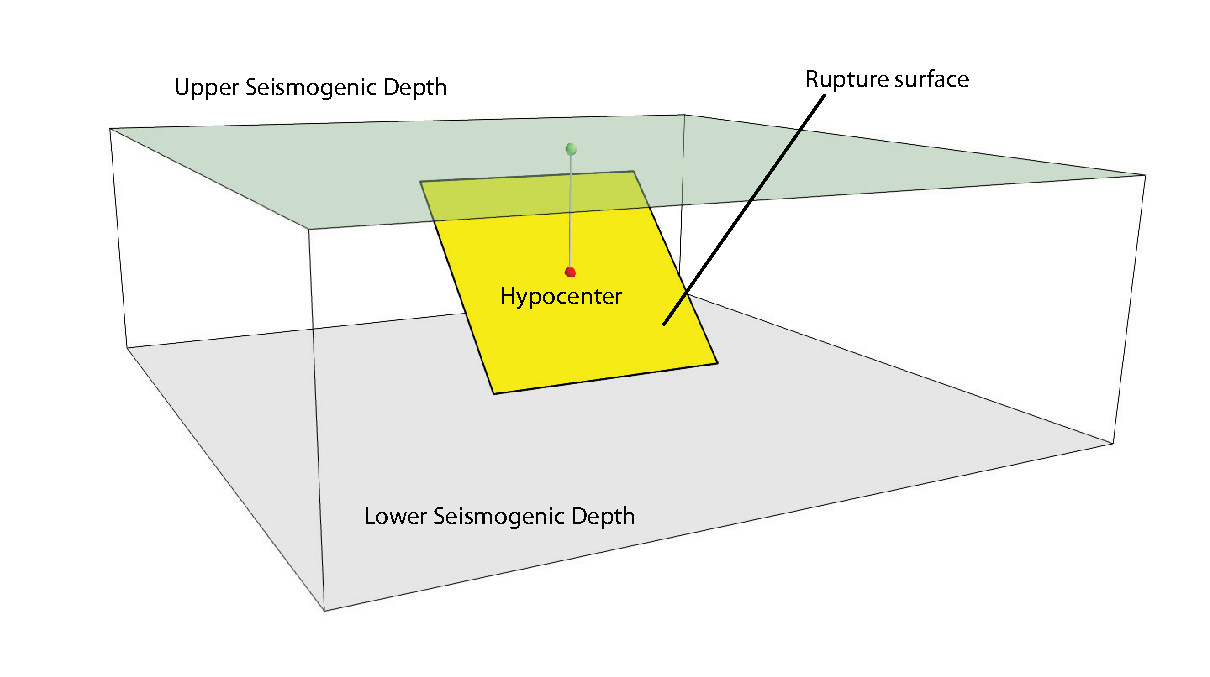
\includegraphics[width=10cm]{figures/hazard/single_rupture.pdf}
	\end{figure}}
}


\newglossaryentry{fragility function}{
	name=fragility function,
	description={the probability of exceeding a set of limit states, given
	an intensity measure level. These functions can be discrete or continuous}
}


\newglossaryentry{fragility model}{
	name=fragility model,
	description={A set of \glspl{fragility function} used to model the
	fragility of all the \glspl{asset} in the \gls{exposure model}}
}


\newglossaryentry{frequencymagnitudedistribution}{
	name=frequency-magnitude distribution,
	description={See \gls{mfd}}
}



% ------- G

\newacronym{acr:gem}{GEM}{Global Earthquake Model}
\newacronym{acr:gmf}{GMF}{Ground Motion Field}
\newacronym{acr:gmpe}{GMPE}{Ground Motion Prediction Equation}
\newacronym{acr:gmlt}{GMLT}{Ground Motion Logic Tree (see \gls{groundmotionlogictree}}


\newglossaryentry{gridsource}{
	name=grid source,
	description={A source typology usually adopted to model distributed
	seismicity. It is routinely produced by a seismicity smoothing algorithm (one
	of the most famous algorithm is the one proposed by \citet{frankel1995})}
}


\newglossaryentry{groundmotionfield}{
	name=ground-motion field,
	description={An object describing the geographic distribution around a
	rupture of a ground motion intensity measure}
}


\newglossaryentry{groundmotionfieldcalc}{
	name=ground-motion field calculator,
	description={An \gls{acr:oqe} calculator that given a rupture computes the
	geographic distribution of a ground motion intensity parameter. Currently
	OQ can generate ground motion fields using a \gls{acr:gmpe}}
}


\newglossaryentry{groundmotionlogictree}{
	name=ground-motion logic tree,
	description={A method used to systematically describe the epistemic
	uncertainties related to the ground motion models used in the computation
	of hazard using a specific \gls{pshainputmodel}}
}


\newglossaryentry{groundmotionmodel}{
	name=ground-motion model,
	description={An object that given a rupture with specific properties
	computes the expected ground motion at the given site. In simplest case a
	ground motion model corresponds to a \gls{groundmotionpredictioneq}. In
	case of complex PSHA input models, the produced ground motion models
	contains a set of \glspl{acr:gmpe}, one for each tectonic region considered}
}


\newglossaryentry{groundmotionparameter}{
	name=ground-motion parameter,
	description={A scalar or vector quantity describing a relevant property
	of the shaking such as intensity (e.g. PGA or Spectral Acceleration)
	or duration, equivalent number of cycles  \citep[see for
	example][]{hancock2005})}
}


\newglossaryentry{groundmotionpredictioneq}{
	name=ground-motion prediction equation,
	description={An equation that - given some fundamental parameters
	characterizing  the source, the propagation path and the site (in the
	simplest  case magnitude, distance and V$_\text{S,30}$) - computes the
	value $GM$ of a (scalar) ground motion intensity parameter}
}


\newglossaryentry{groundmotionsystem}{
	name=ground-motion system,
	description={An object containing a list of \gls{groundmotionlogictree}}
}



% ------- I

\newglossaryentry{initialseismicsourceinputmodel}{
	name=initial seismic source input model,
	description={It is the ensable of information needed to fully describe
	the seismic sources composing a seismic source input model. The
	initial seismic source input model is included in the first  branching
	level of a seismic source logic tree}
}


\newglossaryentry{insured losses}{
	name=insured losses,
	description={Fraction of the ground-up losses that can be covered by the
	insurance industry, according to a certain policy}
}


\newglossaryentry{investigationtime}{
	name=investigation time,
	description={The time interval considered to calculate hazard; usually
	it corresponds to 50 years}
}



% ------- L

\newglossaryentry{limit}{
	name=limit,
	description={A parameter used in the calculation of insured losses that
	establishes the maximum economic amount that can be covered by the insurance
	industry, according to a certain insurance policy}
}


\newglossaryentry{logictree}{
	name=logic tree,
	description={Data structure used to systematically describe uncertainties
	on parameters and models used in a PSHA study}
}


\newglossaryentry{logictreeprocessor}{
	name=logic tree processor,
	description={An OQ calculator that takes the PSHA Input Model and creates
	many realisations of a \gls{seismicsourcemodel} and of a
	\gls{groundmotionmodel}}
}


\newacronym{acr:ltmcs}{LTMCS}{Logic Tree Monte Carlo Sampler}


\newglossaryentry{msr}{
	name=magnitude-scaling relationship,
	description={An empirical relationship linking the magnitude with a
	parameter  describing the size of the corresponding rupture (e.g. the
	area  of the rupture or the rupture length)}
}


\newacronym{acr:mfd}{MFD}{Magnitude-Frequency Distribution}
\newglossaryentry{mfd}{
	name=magnitude-frequency distribution,
	description={A distribution describing the frequency of earthquakes with
	a specific magnitude. It can be continuous or discrete. One frequency-
	magnitude distribution frequently adopted in \gls{acr:psha} is the double
	truncated Gutenberg-Richter distribution}
}



% ------- O

\newacronym{acr:hazlib}{oq-hazardlib}{OpenQuake hazard library}


\newglossaryentry{opensha}{
	name=OpenSHA,
	description={OpenSHA is an open-source, advanced Java-based platform
	for conducting Seismic Hazard Analysis - (see
	\href{http://opensha.org}{OpenSHA website})}
}
\newacronym{acr:oqe}{oq-engine}{OpenQuake-engine}



% ------- P

\newacronym{acr:pga}{PGA}{Peak Ground Acceleration}
\newacronym{acr:pgv}{PGV}{Peak Ground Velocity}

\newacronym[description={\glslink{psha}{Probabilistic Seismic Hazard
	Analysis}}]{acr:psha}{PSHA}{Probabilistic Seismic Hazard Analysis}


\newglossaryentry{pointsource}{
	name=point source,
	description={The elemental source typology used in OpenQuake-engine to
	model distributed seismicity}
}


\newglossaryentry{pshainputmodel}{
	name=PSHA input model,
	description={An object containing the information necessary to describe
	the seismic source and the ground motion models - plus the related
	epistemic uncertainties}
}


\newglossaryentry{psha}{
	name=probabilistic seismic hazard analysis,
	description={A methodology to compute seismic hazard by taking into
	account the potential contributions coming from all the sources of
	engineering importance for a specified site}
}



% ------- R

\newacronym{acr:rrup}{$\text{r}_{\text{rup}}$}{closest distance between the
	site and rupture}


\newglossaryentry{rupture}{
	name=earthquake rupture,
	description={A 3D surface - representing a portion or the entire fault
	surface - over which a slip event (i.e. an earthquake) occurs}
}


\newglossaryentry{ruptureaspectratio}{
	name=rupture aspect ratio,
	description={It is the ratio between the lenght and the width of an
	earthquake rupture}
}


\newglossaryentry{rake}{
	name=rake,
	description={The rake is the direction in which a hanging wall block moves
	during a rupture, measured relative to fault strike on the plane of the
	fault}
}



% ------- S

\newacronym{acr:ssha}{SSHA}{Scenario Based Seismic Hazard Analysis}


\newglossaryentry{scenariohazard}{
	name=scenario based seismic hazard analysis,
	plural=scenario based seismic hazard analyses,
	description={An analyis of seismic hazard based on the selection of
	one or a few ruptures and the computation of the expected ground
	motion at a set of sites using a \gls{gmpe} accounting ground motion
	variability}
}


\newglossaryentry{seismicityhistory}{
	name=seismicity history,
	plural=seismicity histories,
	description={An object containing a set ruptures representative of the
	possible seismicity generated by the sources in a
	\gls{seismicsourcemodel} during the investigation time $t$}
}


\newglossaryentry{seismicityrate}{
	name=seismicity rate,
	description={Number of events per unit of time (if not better
	specified, the definition of a seismicity rate generally presumes a time
	independent}
}


\newglossaryentry{seismicsourcedata}{
	name=seismic source data,
	description={An object containing the information necessary to
	completely describe a \gls{acr:psha} seismic source i.e. seismic source
	type, position, geometry and seismicity occurrence model}
}


\newglossaryentry{seismicsourcelogictree}{
	name=seismic source logic tree,
	description={Logic tree structure defined to describe in structured and
	systematic way the epistemic uncertainties characterizing the seismic
	source model. The first branching level in the logic tree by definition
	contains one or several alternative \gls{initialseismicsourceinputmodel}}
}


\newacronym{acr:ssim}{SSIM}{Seismic Source Input Model}


\newglossaryentry{seismicsourceinputmodel}{
	name=seismic source input model,
	description={An object containing a list of \gls{seismicsourcedata}. In
	the OpenQuake-engine a seismic source model doesn't contain epistemic
	uncertainty}
}


\newglossaryentry{seismicsource}{
	name=seismic source,
	description={An object that can generate}}


\newacronym{acr:ssm}{SSM}{Seismic Source Model}
\newglossaryentry{seismicsourcemodel}{
	name=seismic source model,
	description={An object containing a list of \glspl{seismicsource}
	objects}
}


\newacronym{acr:scec}{SCEC}{Southern California Earthquake Center}


\newglossaryentry{seismicsourcesystem}{
	name=seismic source system,
	description={An object containing a list of
	\glspl{initialseismicsourceinputmodel} and the
	\gls{seismicsourcelogictree}}
}


\newglossaryentry{simplefaultsource}{
	name=simple fault source,
	description={A source typology usually adopted to model shallow
	structures with an uncomplicated geometry}
}


\newacronym{acr:ses}{SES}{Stochastic Event Set}
\newglossaryentry{stochasticeventset}{
	name=stochastic event set,
	description={An object containing one or many \glspl{seismicityhistory}}
}


\newglossaryentry{strike}{
	name=strike,
	description={The strike direction correspond to the angle between the
	north and the direction you take so that when you walk along the
	\gls{faulttrace} the fault dips on your right}
}


\newacronym{acr:sa}{S$_a$}{Spectral Acceleration}



% ------- T

\newglossaryentry{taxonomy}{
	name=taxonomy,
	plural=taxonomies,
	description={Scheme used to classify the \glspl{asset}. For buildings, a
	classification scheme has been proposed by \gls{acr:gem} which considers a
	number of attributes including lateral load resisting system and its
	material, height, year of construction. The taxonomy is currently used to
	link the \glspl{asset} in the \gls{exposure model} to the relevant
	\gls{vulnerability function} or \gls{fragility function}}
}


\newglossaryentry{tectonicregion}{
	name=tectonic region,
	description={A area on the topographic surface that can be considered
	homogeneous in terms of tectonic properties such as the prevalent
	seismogenic properties and/or the seismic wave propagation properties}
}


\newglossaryentry{temporaloccurrencemodel}{
	name=temporal occurrence model,
	description={Usually a probabilistic model giving the probability of
	occurrence of an event in a specified \gls{investigationtime}}
}



% ------- U

\newacronym{acr:usgs}{USGS}{United States Geological Survey}



% ------- V

\newglossaryentry{vulnerability function}{
	name=vulnerability function,
	description={A function that describes the probability distribution of
	loss ratio, conditioned on an intensity measure level. Currently only
	discrete vulnerability functions are supported}
}


\newglossaryentry{vulnerability model}{
	name=vulnerability model,
	description={A set of \glspl{vulnerability function} used to model the
	physical vulnerability of all the \glspl{asset} in the \gls{exposure model}}
}


\newglossaryentry{acr:vs30}{
	name=V$_{S,30}$,
	description={Average shear wave velocity of the materials in the uppermost
	30m of the soil column}
} % ---------------------------------------- Load glossary -

%-------------------------------------------------------------------------------
%  COVER PAGE
%-------------------------------------------------------------------------------

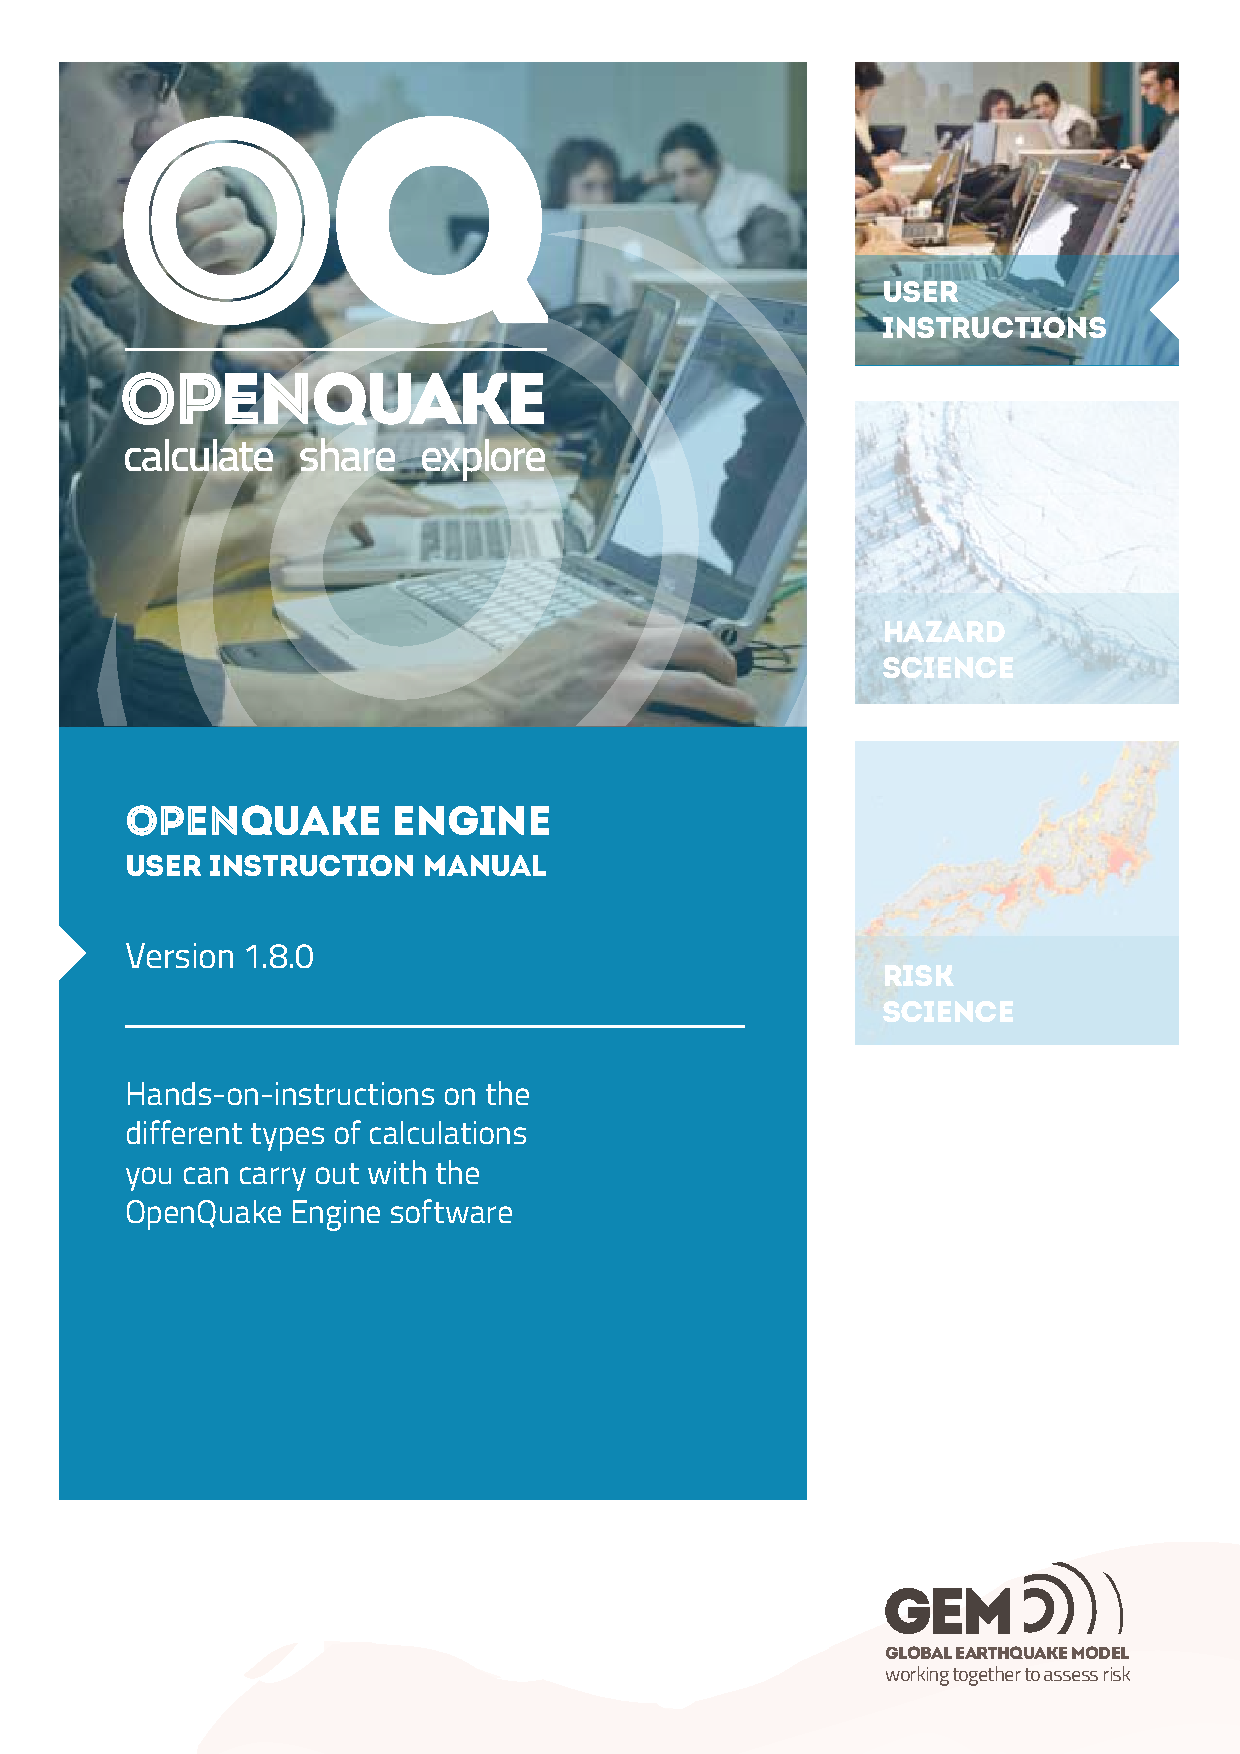
\includepdf[pages=-]{figures/oq_manual_cover.pdf}

%-------------------------------------------------------------------------------
%  TITLE PAGE
%-------------------------------------------------------------------------------

\begingroup
\thispagestyle{empty}
\begin{center}
\par\normalfont\fontsize{15}{15}\sffamily\selectfont
\textcolor{oqblue}{OpenQuake: calculate, share, explore}
\vspace*{9cm}
\par\bfseries\fontsize{35}{35}\sffamily\selectfont
\textcolor{gembrown}{The OpenQuake-engine\\User Instruction Manual}\par
\vspace*{9cm}
\par\normalfont\fontsize{15}{15}\sffamily\selectfont
\href{http://globalquakemodel.org/openquake/}{\textcolor{oqblue}{globalquakemodel.org/openquake}}
\end{center}
\endgroup

%-------------------------------------------------------------------------------
%  COPYRIGHT PAGE
%-------------------------------------------------------------------------------

\newpage
~\vfill
\thispagestyle{empty}

\noindent
   \textbf{Authors} \\
   Marco Pagani$^1$, Vitor Silva$^1$, Graeme Weatherill$^1$,
   Anirudh Rao$^1$, Michele Simionato$^1$\hfill \\
   \hfill \\
   \textbf{Authors on previous versions} \\
   Helen Crowley$^2$, Damiano Monelli\hfill \\
   \hfill \\
   \small
   \begin{tabular}{p{4cm}p{4cm}p{4cm}}
   $^1$ GEM Foundation \hfill \newline
   via Ferrata, 1 \hfill \newline
   20133 Pavia \hfill \newline
   Italy \hfill \newline
   &
   $^2$ EUCENTRE \hfill \newline
   via Ferrata, 1 \hfill \newline
   20133 Pavia \hfill \newline
   Italy \hfill \newline
   \end{tabular} \hfill \newline
   %
   Email address for all the authors:\hfill\\
   $<$name.surname$>$@globalquakemodel.org\hfill\\
   \normalsize

\noindent
   {\textbf{Citation}} \hfill \\
   Please cite this document as: \hfill \\
   GEM (2016). The OpenQuake-engine User Manual.
   \textit{Global Earthquake Model (GEM) Technical Report 2016-06.\\
   doi: 10.13117/GEM.OPENQUAKE.MAN.ENGINE.2.0/01, 193 pages.} \hfill \\
\noindent \hfill\\
\noindent
   {\bf{Disclaimer}} \hfill \\
   The OpenQuake-engine User Manual is distributed in the hope that it will be
   useful, but without any warranty: without even the implied warranty of
   merchantability or fitness for a particular purpose. While every precaution
   has been taken in the preparation of this document, in no event shall the
   authors of the Manual and the GEM Foundation be liable to any party for
   direct, indirect, special, incidental, or consequential damages, including
   lost profits, arising out of the use of information contained in this
   document or from the use of programs and source code that may accompany it,
   even if the authors and GEM Foundation have been advised of the possibility
   of such damage. The Manual provided hereunder is on as ``as is'' basis, and
   the  authors and GEM Foundation have no obligations to provide maintenance,
   support, updates, enhancements, or modifications. \hfill \\
\noindent \hfill\\
\noindent
   {\bf{License}} \hfill \\
   This Manual is distributed under the Creative Commons License  Attribution-
   NonCommercial-ShareAlike 4.0 International
   (\href{http://creativecommons.org/licenses/by-nc-sa/4.0/} {CC BY-NC-SA
   4.0}). You can download this Manual and share it with others as long as you
   provide proper credit, but you cannot change it in any way or use it
   commercially.\hfill \\

\noindent \copyright\ \textsc{2013--2016 GEM Foundation}\\
\noindent \textit{Ninth printing, June 2016} % Printing/edition date

%-------------------------------------------------------------------------------
%  TABLE OF CONTENTS
%-------------------------------------------------------------------------------

\chapterimage{figures/chapter_head.pdf} % Table of contents heading image
\pagestyle{empty} % No headers
\tableofcontents % Print the table of contents itself
\cleardoublepage % Forces the first chapter to start on the right
\pagestyle{fancy} % Print headers again

%-------------------------------------------------------------------------------
%  FOREWORD
%-------------------------------------------------------------------------------
\chapterimage{figures/chapter_head.pdf} % Chapter heading image
\chapter*{Preface}
\addcontentsline{toc}{chapter}{Preface}
%-------------------------------------------------------------------------------
The goal of this manual is to provide a comprehensive and transparent description
of the features of the OpenQuake-engine (v1.2). This manual is designed to be 
readable by someone with basic understanding of Probabilistic Seismic Hazard 
and Risk Analysis, but no previous knowledge of the OpenQuake-engine is assumed.
%
The OpenQuake-engine is an effort promoted and actively developed by the
Global Earthquake Model, a public-private partnership initiated by the Global
Science Forum of the Organisation for Economic Co-operation and Development 
(OECD)\footnote{A short description of the process promoted by OECD is available 
here http://www.oecd.org/science/sci-tech/theglobalearthquakemodelgem.htm}.

The OpenQuake-engine is the result of an effort carried out jointly by the
Information Technology and Scientific teams working at the GEM Secretariat. 
It is freely distributed under an Affero GPL license 
(more information available at this link 
\href{http://www.gnu.org/licenses/agpl-3.0.html}{http://www.gnu.org/licenses/agpl-3.0.html})


%-------------------------------------------------------------------------------
%  THE MANUAL
%-------------------------------------------------------------------------------

% ------------------------------------------------------- Part I: Introduction -
\part{Introduction}
\label{part:introduction}
\chapterimage{figures/chapter_head.pdf} % Chapter heading image
\chapter{OpenQuake-engine Background}
   \label{chap:intro}
	OpenQuake-engine is the seismic hazard and risk calculation software developed by
the \glsdesc{acr:gem}. By following current standards in software
developments like test-driven development and continuous integration, the
\glsdesc{acr:oqe} aims at becoming an open, and community-driven tool for
seismic hazard and risk analysis.

The source code of the \glsdesc{acr:oqe} is available on a public web-based
repository at the following address:

\href{http://github.com/gem/oq-engine}{http://github.com/gem/oq-engine}.


% ------------------------------------------------------------------------------
\section{Running the OpenQuake-engine}
\index{Running OpenQuake!introduction}
\label{sec:running_oq_engine}

An \gls{acr:oqe} analysis is launched from the command line of a terminal.

A schematic list of the options that can be used for the execution of the
\gls{acr:oqe} can be obtained with the following command:

\begin{minted}[fontsize=\footnotesize,frame=single,bgcolor=lightgray]{shell-session}
user@ubuntu:~\$ oq-engine --help
\end{minted}

The result is the following:

\inputminted[firstline=1,fontsize=\footnotesize,frame=single]{shell-session}{oqum/help.txt}\\

% ----------------------------------------------------- Part II: Hazard Module -
\thispagestyle{empty}
\part{Hazard}

\chapterimage{figures/chapter_head.pdf} % Chapter heading image
\chapter{Introduction to the Hazard Module}
   \label{chap:hazintro}
	\index{OpenQuake-engine!hazard}

The hazard component of the OpenQuake-engine builds on top of the
\gls{acr:hazlib}, a Python-based library containing tools for PSHA
calculations.

The web repository of this library is available at the following address:\\
\href{http://github.com/gem/oq-hazardlib}{http://github.com/gem/oq-hazardlib}.

In this section we briefly illustrate the main properties of the hazard
component of the OpenQuake-engine. In particular, we will describe the main
typologies of sources supported and the main calculation workflows available.


\section{Source typologies}
\index{Source type}
\label{sec:source_typologies}
An \gls{acr:oqe} \gls{seismicsourceinputmodel} contains a list of sources
belonging to a finite set of possible typologies. Each source type is defined
by a set of parameters - called source data - which are used to specify the
source geometry and the properties of seismicity occurrence.

Currently the \gls{acr:oqe} supports the following source types:

\begin{itemize}

    \item Sources for modelling distributed seismicity:

    \begin{itemize}

        \item \Gls{pointsource} - The elemental source type used to model
        distributed seismicity. Grid and area sources (described below) are
        different containers of point sources.

        \item \Gls{areasource} - So far, the most frequently adopted source
        type in national and regional PSHA models.

        \item \Gls{gridsource} - A replacement for area sources admitting
        spatially variable seismicity occurrence properties.

    \end{itemize}

    \item Fault sources with floating ruptures:

    \begin{itemize}

        \item \Gls{simplefaultsource} - The simplest fault model in the
        OpenQuake-engine. This source is habitually used to describe shallow
        seismogenic faults.

        \item \Gls{complexfaultsource} - Often used to model subduction
        interface sources with a complex geometry.

    \end{itemize}

    \item Fault sources with ruptures always covering the entire fault surface:

    \begin{itemize}

        \item \Gls{charfaultsource} - A typology of source where ruptures
        always fill the entire fault surface.

    \end{itemize}

\end{itemize}

The OpenQuake-engine contains some basic assumptions for the definition of
these source typologies:

\begin{itemize}

    \item In the case of area and fault sources, the seismicity is
    homogeneously distributed over the source;

    \item Seismicity temporal occurrence follows a Poissonian model.

\end{itemize}

The above sets of sources may be referred to as ``parametric'' sources, that is to say that the generation of the \Gls{earthquakeruptureforecast} is done by the OpenQuake engine based on the parameters of the sources set by the user. In some cases, particularly if the user wishes for the temporal occurrence model to be non-Poissonian (such as the lognormal or Brownian Passage Time models) a different type of behaviour is needed. For this OpenQuake-engine supports a \Gls{nonparametricsource} in which the \Gls{earthquakeruptureforecast} is provided explicitly by the user as a set of ruptures and their corresponding probabilities of occurrence.

\subsection{Source typologies for modelling distributed seismicity}
\subsubsection{Point sources}
\label{subsubsec:point_sources}
\index{Source type!point}
\index{Point source|see{Source type}}

\begin{figure}[!ht]
\centering
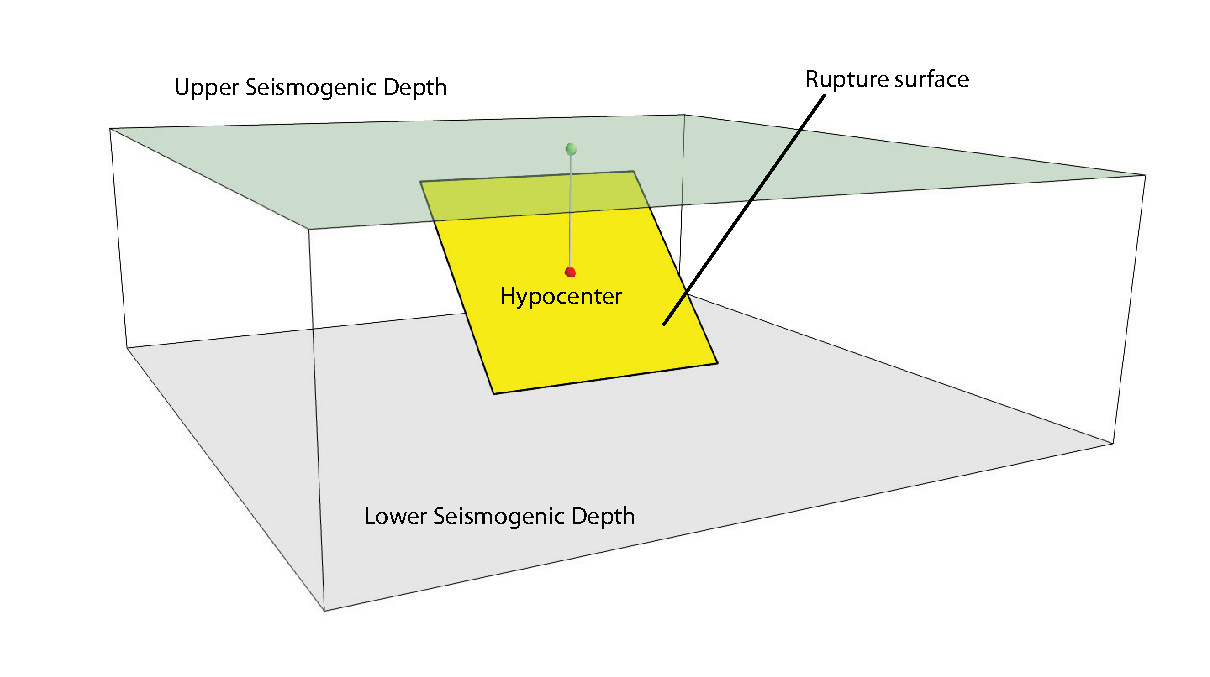
\includegraphics[width=10cm]{figures/hazard/single_rupture.pdf}
\caption{Single rupture}
\label{fig:single_rupture}
\end{figure}

The point source is the elemental source type adopted in the OpenQuake-engine
for modelling distributed seismicity. The OpenQuake-engine always performs
calculations considering finite ruptures, even in the case of point sources.

These are the basic assumptions used to generate ruptures with point sources:

\begin{itemize}

    \item Ruptures have a rectangular shape

    \item Rupture hypocenter is located in the middle of the rupture

    \item Ruptures are limited at the top and at the bottom by two planes
    parallel to the topographic surface and placed at two characteristic
    depths named upper and lower seismogenic depths, respectively (see
    Figure~\ref{fig:single_rupture})

\end{itemize}

\paragraph{Source data}

For the definition of a point source the following parameters are required
(Figure~\ref{fig:single_rupture} shows some of the parameters described
below, together with an example of the surface of a generated rupture):

\begin{itemize}

    \item The coordinates of the point (i.e. longitude and latitude) [decimal
    degrees]

    \item The upper and lower seismogenic depths [km]

    \item One \gls{mfd}

    \item One magnitude-scaling relationship

    \item The rupture aspect ratio

    \item A distribution of nodal planes i.e. one (or several) instances
    of the following set of parameters:

    \begin{itemize}
        \item \gls{strike} [degrees]
        \item \gls{dip} [degrees]
        \item \gls{rake} [degrees]
    \end{itemize}

\item A magnitude independent depth distribution of hypocenters [km].

\end{itemize}

Figure~\ref{fig:point_source_multiple_ruptures} shows ruptures generated by a
point source for a range of magnitudes. Each rupture is centered on the
single hypocentral position admitted by this point source. Ruptures are
created by conserving the area computed using the specified magnitude-area
scaling relatioship and the corresponding value of magnitude.

\begin{figure}[ht!]
\centering
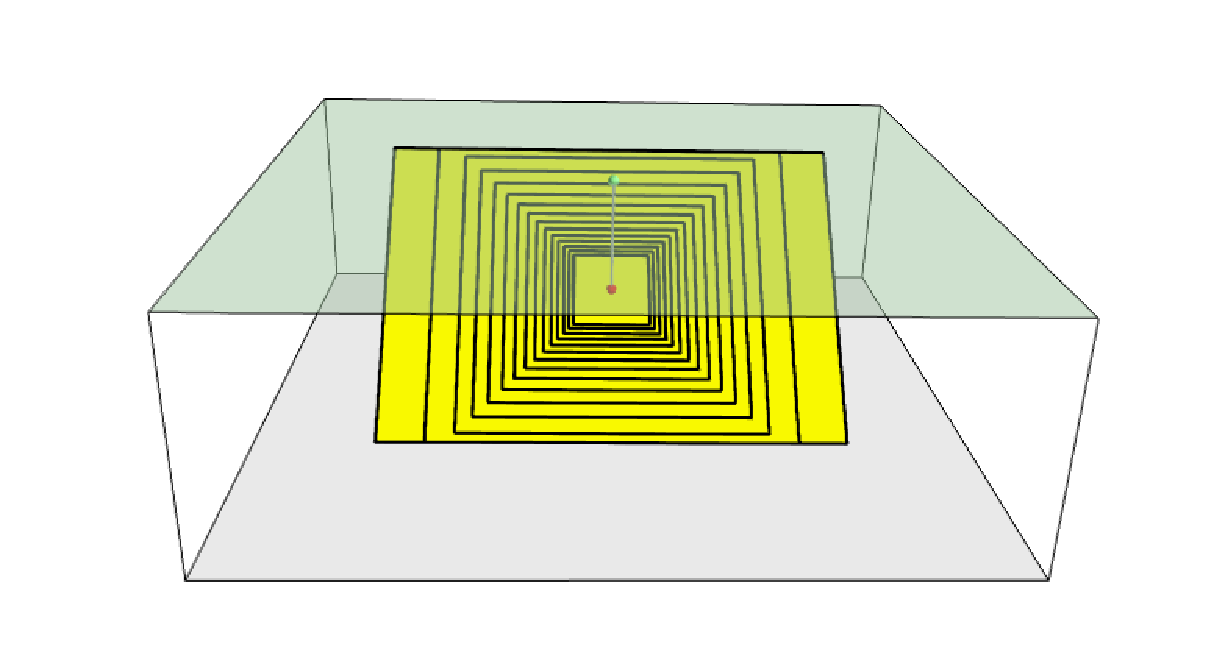
\includegraphics[width=10cm]{figures/hazard/point_source_multiple_ruptures.pdf}
\caption{Point source with multiple ruptures. Note the change in the aspect
ratio once the rupture width fills the entire seismogenic layer.}
\label{fig:point_source_multiple_ruptures}
\end{figure}

Below we provide the excerpt of an .xml file used to describe the properties
of a point source:

\input{oqum/hazard/verbatim/input_point_source}
\label{page:point_source_nrml}

The red part shows the the parameters used to describe the geometry of the
point source, the blue part is the description of the magnitude-frequency
distribution, the green text shows the nodal plane distribution and the text
in magenta illustrates the hypocentral depth distribution.

The text in black describes the parameters needed to generate the ruptures
such as the \gls{msr} and the aspect ratio.

Note that in this example, ruptures occur on two possible nodal planes and
two hypocentral depths. Figure~\ref{fig:point_source_ruptures} shows the
ruptures generated by the point source specified above.

\begin{figure}[!ht]
\centering
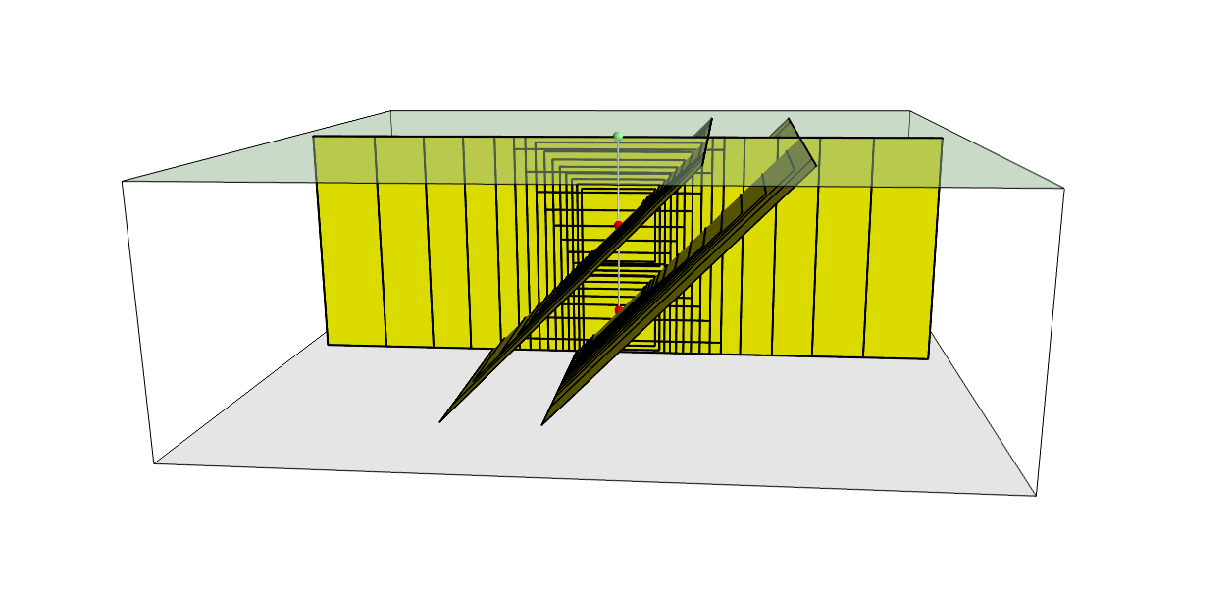
\includegraphics[width=10cm]{figures/hazard/pointsrc_2strike_2hypodep.pdf}
\caption{Ruptures produced by the source created using the information 
in the example .xml file described at page~\pageref{page:point_source_nrml}.}
\label{fig:point_source_ruptures}
\end{figure}



\subsubsection{Grid sources}
\label{subsubsec:grid_sources}
\index{Source type!grid}
\index{Grid source|see{Source type}}

A \gls{gridsource} is simply a collection of point sources distributed over a
regular grid (usually equally spaced in longitude and latitude).

In \gls{psha} a grid source can be considered a model alternative to area
sources, since they both model distributed seismicity.

Grid sources are generally used to reproduce more faithfully the spatial
pattern of seismicity depicted by the earthquakes occurred in the past; in
some models (e.g. \citet{petersen2008}) only events of low and intermediate
magnitudes are considered.

Grid sources are generally computed using seismicity smoothing algorithms
\citep[][amongst many others]{frankel1995,woo1996}.

The use of smoothing algorithms to produce grid sources brings some
advantages compared to area sources, since (1) it removes most of the
unavoidable degree of subjectivity due to the definition of the geometries of
the area sources and (2) it produces a spatial pattern of seismicity that is
usually closer to what observed in the reality. Nevertheless, in many cases
smoothing algorithms require an a-priori definition of some setup parameters
that expose the calculation to a certain degree of partiality.

Grid sources are modeled in \gls{acr:oqe} simply as a set of point sources; in
other words, a grid source is just a long list of point sources specified as
described in the previous section (see page
\pageref{subsubsec:point_sources}).



\subsubsection{Area sources}
\label{subsubsec:area_sources}
\index{Source type!area}
\index{Area source|see{Source type}}

Area sources are usually adopted to describe the seismicity occurring over
wide areas where the identification and characterization - i.e. the
unambiguous definition of position, geometry and seismicity occurrence
parameters - of single fault structures is difficult.

From a computation standpoint, area sources are comparable to grid sources
since they are both represented in the engine by a list of point sources.

The \gls{acr:oqe} using the source data parameters (see below) creates an
equally spaced in distance grid of point sources where each point has the same
seismicity occurrence properties (i.e. rate of events generated).

Below we provide a brief description of the parameters necessary to completely
describe an area source.

\paragraph{Source data}

\begin{itemize}

    \item A polygon defining the external border of the area (i.e. a list of
    Longitude-Latitude [degrees] tuples) The current version of the OQ-engine doesn't
    support the definition of internal borders.

    \item The upper and lower seismogenic depths [km]

    \item One gls{mfd}

    \item One gls{msr}

    \item The rupture aspect ratio

    \item A distribution of nodal planes i.e. one (or several) instances of
    the following set of parameters

    \begin{itemize}
        \item \gls{strike} [degrees]
        \item \gls{dip} [degrees]
        \item \gls{rake} [degrees]
    \end{itemize}

    \item A magnitude independent depth distribution of hypocenters [km].

\end{itemize}

Below we provide the exerpt of an .xml file used to describe the properties of
an area source:

\input{oqum/hazard/verbatim/input_area_source}

The red text describes the parameters used to describe the geometry of the
area source; the blue part is the description of the magnitude-frequency
distribution; the green text displays the nodal plane distribution; and the
text in magenta illustrates the hypocentral depth distribution.

The text in gray describes the parameters required to generate the ruptures
such as the \gls{msr} and the aspect ratio.

The ruptures generated by the area source described in the example above are
controlled by two nodal planes and have hypocenters at localized at two
distinct depths.

\subsection{Fault sources with floating ruptures}
Fault sources in the \gls{acr:oqe} are classified according to the method
adopted to distribute ruptures over the fault surface. Two options are
currently supported:

\begin{itemize}

    \item With the first option, ruptures with a surface lower than the
    whole fault surface are floated so as to cover as much as possible
    homogeneously the fault surface. This model is compatible with all the
    supported magnitude-frequency distributions.

    \item With the second option, ruptures always fill the entire fault
    surface. This model is compatible with magnitude-frequency
    distributions similar to a characteristic model (\`{a} la
    \cite{schwartz1984}).

\end{itemize}

In this subsection we discuss the different fault source types that
support floating ruptures. In the next subsection we will illustrate the fault
typology available to model a characteristic rupturing behaviour.



\subsubsection{Simple faults}
\label{desc_simple_fault}
\index{Source type!fault!simple geometry}
\index{Simple fault|see{Source type}}

Simple Faults are the most common source type used to model shallow faults;
the ``simple'' adjective relates to the geometry description of the source
which is obtained by projecting the fault trace (i.e. a polyline) along a
characteristic dip direction.

The parameters used to create an instance of this source type are described
in the following paragraph.

\paragraph{Source data}

\begin{itemize}

    \item A \gls{faulttrace} (usually a polyline). It is a list of
    longitude-latitude tuples [degrees]

    \item A \gls{frequencymagnitudedistribution}

    \item A \gls{msr}

    \item A representative value of the dip angle (specified following
    the Aki-Richards convention; see \citet{aki2002}) [degrees]

    \item Rake angle (specified following the Aki-Richards convention;
    see \citet{aki2002}) [degrees]

    \item Upper and lower depth values limiting the seismogenic interval [km]

\end{itemize}

For near-fault probabilistic seismic hazard analysis, two additional
parameters are needed for characterising seismic sources:

\begin{itemize}

    \item A hypocentre list. It is a list of the possible hypocentral
    positions, and the corresponding weights, e.g., alongStrike="0.25"
    downDip="0.25" weight="0.25". Each hypocentral position is defined in
    relative terms using as a reference the upper left corner of the rupture
    and by specifying the fraction of rupture length and rupture width.

    \item A slip list. It is a list of the possible rupture slip directions
    [degrees], and their corresponding weights. The angle describing each slip
    direction is measured counterclockwise using the fault strike direction as
    reference.

\end{itemize}

In near-fault PSHA calculations, the hypocentre list and the slip list are
mandatory. The weights in each list must always sum to one. The available GMPE
which currently supports the near-fault directivity PSHA calculation in OQ-
engine is the ChiouYoungs2014NearFaultEffect GMPE developed  by
\citet{chiou2014update} (associated with an \texttt{Active Shallow Crust}
tectonic region type).

Below we provide two examples of simple fault source files. The first is an
excerpt of an xml file used to describe the properties of a simple fault
source and the second example shows the excerpt of an xml file used to
describe the properties of a simple fault source that can be used to perform a
PSHA calculation taking into account directivity effects.

\input{oqum/hazard/verbatim/input_simple_fault}
\label{example_incremental_mfd}

Below is an excerpt of a simple fault source xml file for near-fault
directivity PSHA calculations:

\input{oqum/hazard/verbatim/input_simple_fault_directivity}

As with the previous examples, the red text highlights the parameters used to
specify the source geometry, the parameters in green describe the rupture
mechanism, the text in blue describes the magnitude-frequency distribution and
the gray text describes the rupture properties.



\subsubsection{Complex faults}
\label{desc_complex_fault}
\index{Source type!fault!complex geometry}
\index{Complex fault|see{Source type}}

A complex fault differs from simple fault just by the way the geometry of the
fault surface is defined and the fault surface is later created. The input
parameters used to describe complex faults are, for the most part, the same
used to describe the simple fault typology.

In case of complex faults the dip angle is not requested while the fault trace
is substituted by two fault edges limiting at the top and bottom the fault
surface. Additional curves lying over the fault surface can be specified to
complement and refine the description of the fault surface geometry.

Usually, we use complex faults to model intraplate megathrust faults such as
the big subduction structures active in the Pacific (Sumatra, South America,
Japan) but this source typology can be used also to create - for example -
listric fault sources with a realistic geometry.

\input{oqum/hazard/verbatim/input_complex_fault}

As with the previous examples, the red text highlights the parameters used to
specify the source geometry, the parameters in green describe the rupture
mechanism, the text in blue describes the magnitude-frequency distribution and
the gray text describes the rupture properties.


\subsection{Fault sources without floating ruptures}
\subsubsection{Characteristic faults}
\index{Source type!fault!characteristic}
\index{Characteristic fault|see{Source type}}

The charactercistic fault source is a particular typology of fault created
with the assumption that its ruptures will always cover the entire fault
surface.

In this case, the fault surface can be represented either as a
\gls{simplefaultsource} surface or as a \gls{complexfaultsource} surface or as
a combination of rectangular ruptures as represented in
Figure~\ref{fig:char_fault_source}.

\begin{figure}[!ht]
\centering
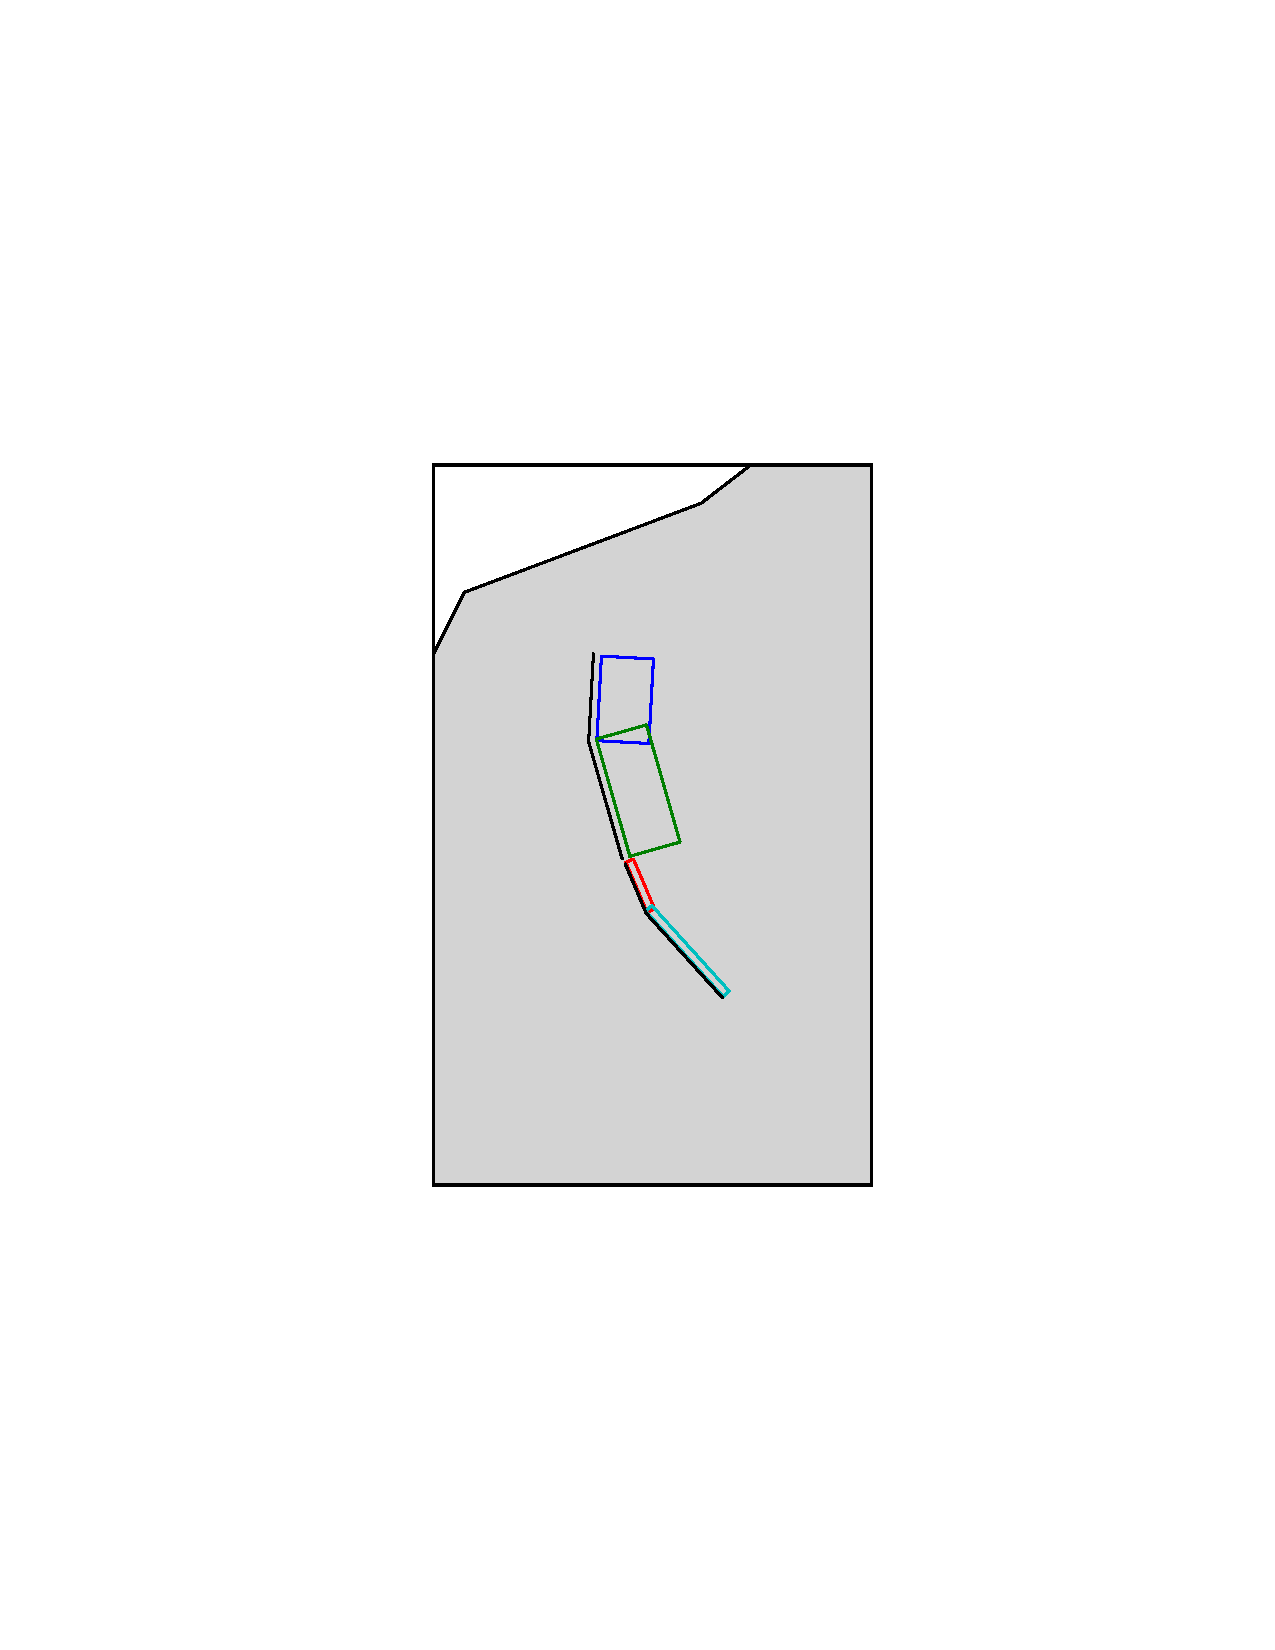
\includegraphics[width=15cm]{figures/hazard/multi_surface.pdf}
\caption{Geometry of a multi-segmented characteristic fault composed of four
         rectangular ruptures as modelled in OpenQuake.}
\label{fig:char_fault_source}
\end{figure}

\paragraph{Source data}

\begin{itemize}

    \item The characteristic rupture surface is defined through one of the
    following options:

        \begin{itemize}

            \item A list of rectangular ruptures

            \item A \gls{simplefaultsource} geometry

            \item A \gls{complexfaultsource} geometry

        \end{itemize}

    \item A \gls{frequencymagnitudedistribution}.

    \item Rake angle (specified following the Aki-Richards convention; see
          \citet{aki2002}).

    \item Upper and lower depth values limiting the seismogenic interval.

\end{itemize}



\section{Magnitude-frequency distributions}
\label{sec:mfd_list}
\subsection{Supported magnitude-frequency distributions}
\label{sec:mfd}
The magnitude-frequency distributions currently supported by the 
\gls{acr:oqe} are the following: 
\begin{description}
    \item[A discrete incremental magnitude-frequency distribution] \hfill \\
    It's the simplest distribution offered. It's defined by a 
    minimum value of magnitude (representing the mid point of the first
    bin) and the bin width. The distribution itself is simply a 
    sequence of floats describing the annual number of events for 
    different bins (centered on increasing values of magnitude). 
    Below we show an example of the xml used to describe an incremental 
    \glspl{acr:mfd} for a seismic source input of a \gls{acr:ssim}.
\begin{Verbatim}[frame=single, commandchars=\\\{\}, fontsize=\footnotesize]
<incrementalMFD minMag="5.05" binWidth="0.1">
    <occurRates>0.15 0.08 0.05 0.03 0.015</occurRates>
</incrementalMFD>
\end{Verbatim}
    This is the magnitude-frequency distribution obtained with the above
    settings:
% ..............................................................................
% . . . . . . . . . . . . . . . . . . . . . . . . . . . . . . . . . . . > Figure
\begin{figure}[!ht]
\centering
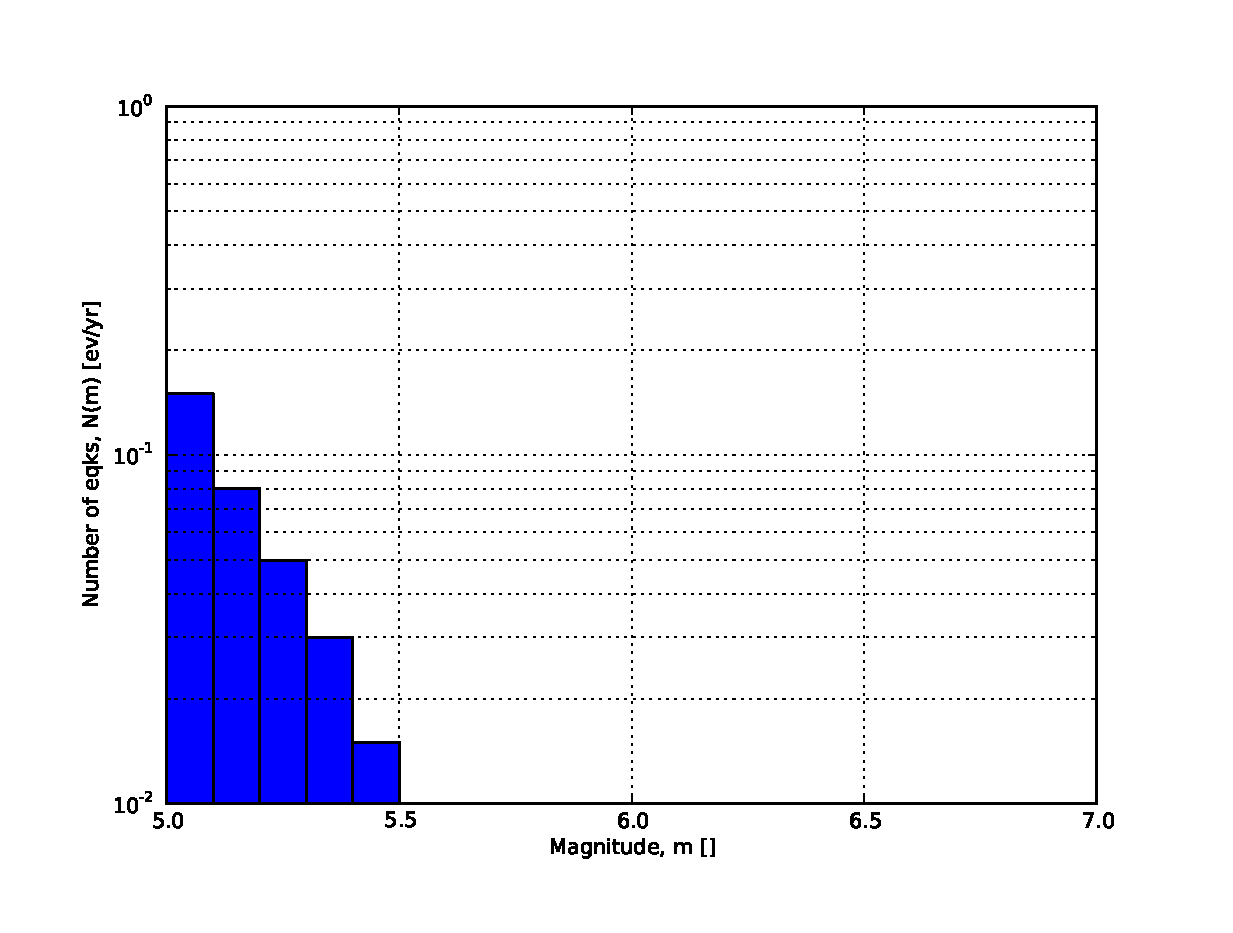
\includegraphics[width=12cm]{./figures/hazard/ed_mfd.eps}
\caption{Incremental magnitude-frequency distribution.}
\label{fig:evenly_discretized_mfd}
\end{figure}
% . . . . . . . . . . . . . . . . . . . . . . . . . . . . . . . . . . . < Figure
% ..............................................................................
%
\item[A double truncated Gutenberg-Richter distribution] \hfill \\
    This distribution is de\-scribed by means of a minimum \texttt{minMag}
    and maximum magnitude \texttt{maxMag} and by the $a$ and $b$ values 
    of the Gutenberg-Richter relationship. The synthax of the xml is 
    rather compact as shown below
\begin{Verbatim}[frame=single, commandchars=\\\{\}, fontsize=\footnotesize]
<truncGutenbergRichterMFD aValue="5.0" bValue="1.0" minMag="5.0" 
        maxMag="6.0"/>
\end{Verbatim}
    This is the magnitude-frequency distribution obtained using the 
    parameters of the considered example:
% ..............................................................................
% . . . . . . . . . . . . . . . . . . . . . . . . . . . . . . . . . . . > Figure
\begin{figure}[!ht]
\centering
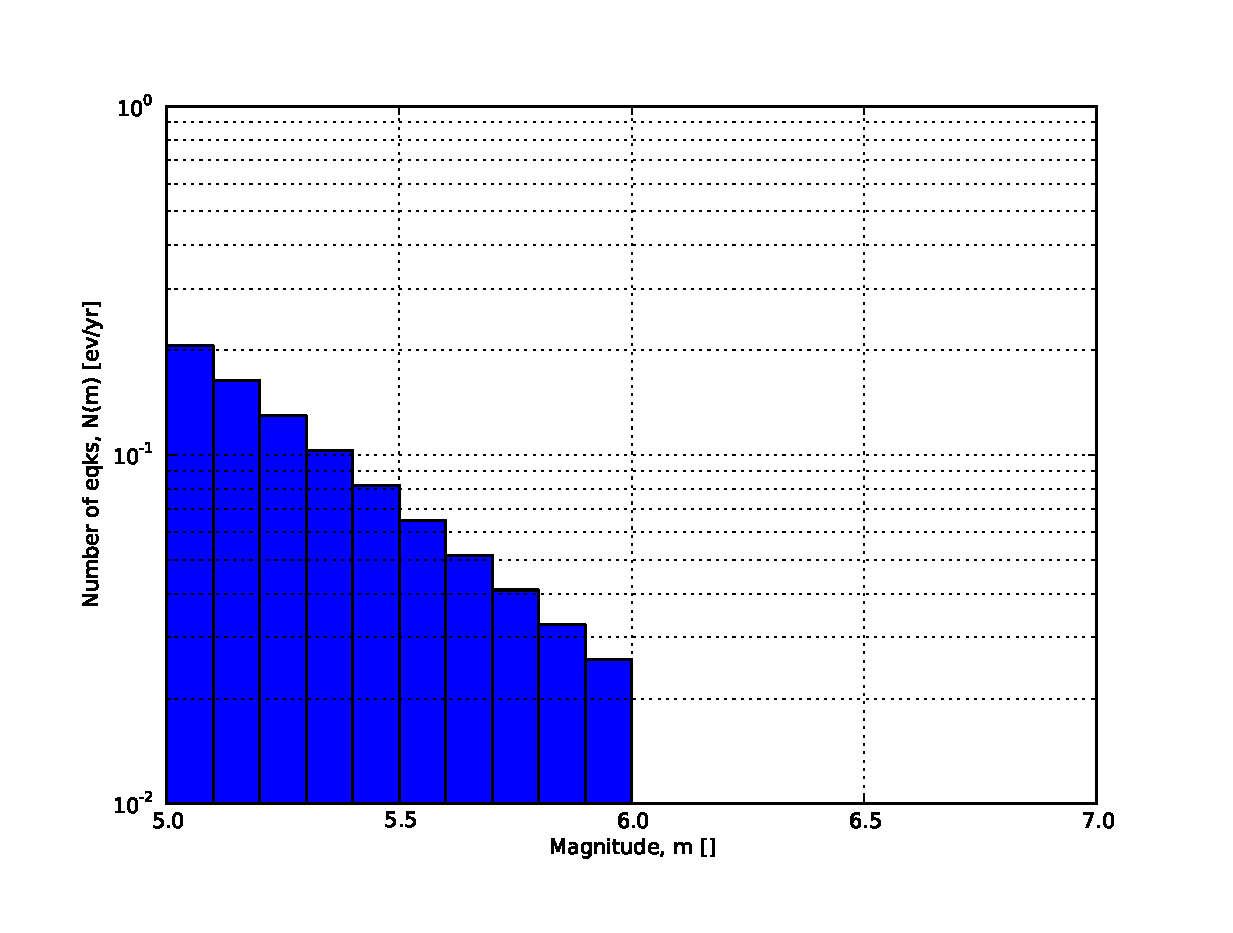
\includegraphics[width=12cm]{./figures/hazard/dt_mfd.eps}
\caption{Double truncated Gutenberg-Richter magnitude-frequency distribution.}
\label{fig:dt_gr_mfd}
\end{figure}
% . . . . . . . . . . . . . . . . . . . . . . . . . . . . . . . . . . . < Figure
% ..............................................................................
%
\item[Characteristic earthquake model (\`{a} la \cite{youngs1985})]
    The 
\begin{Verbatim}[frame=single, commandchars=\\\{\}, fontsize=\footnotesize]
    AA
\end{Verbatim}
% ..............................................................................
% . . . . . . . . . . . . . . . . . . . . . . . . . . . . . . . . . . . > Figure
\begin{figure}[!ht]
\centering
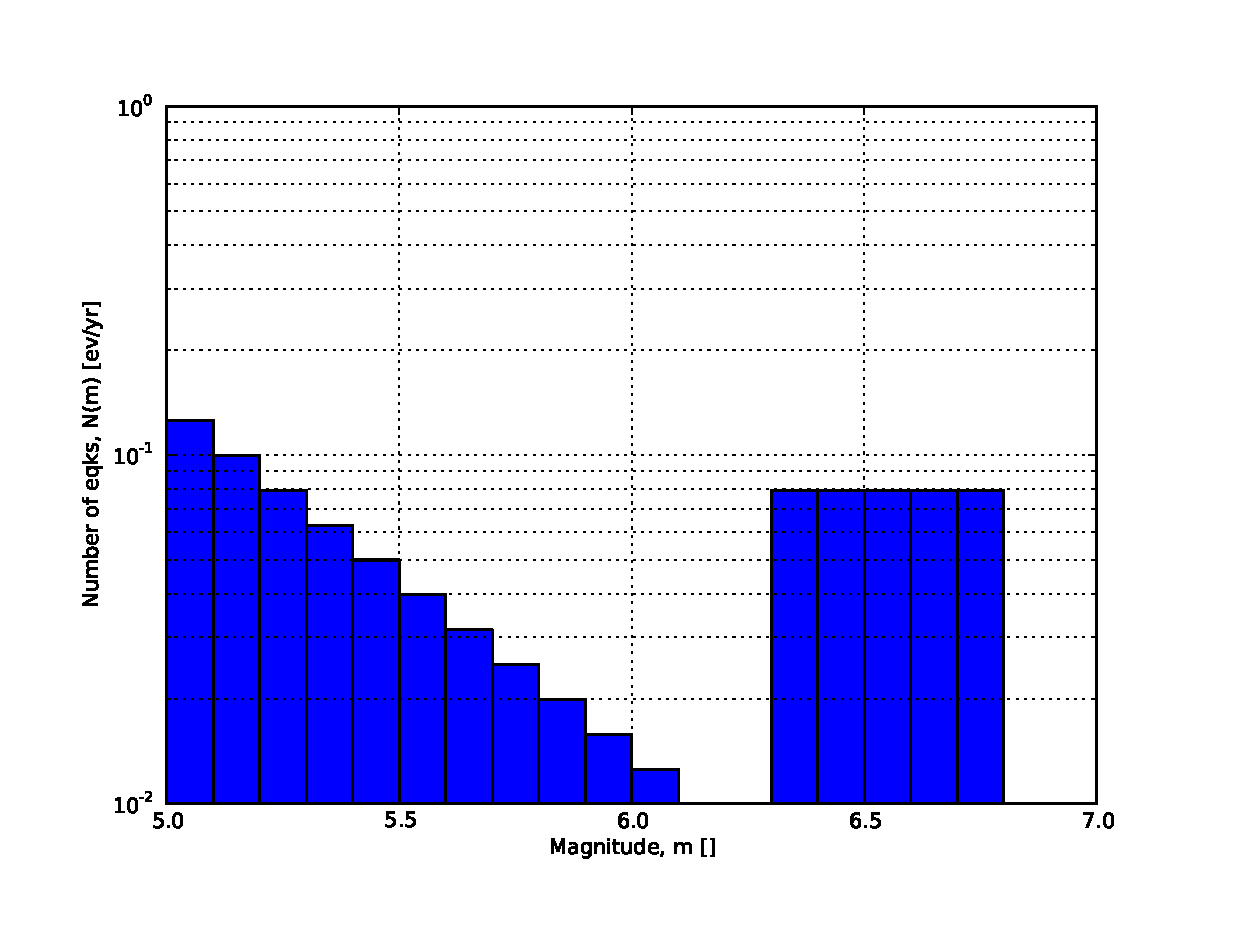
\includegraphics[width=12cm]{./figures/hazard/yc_mfd.eps}
\caption{\cite{youngs1985} magnitude-frequency distribution.}
\label{fig:yc_gr_mfd}
\end{figure}
% . . . . . . . . . . . . . . . . . . . . . . . . . . . . . . . . . . . < Figure
% ..............................................................................

\end{description}


\section{Magnitude-scaling relationships}
\label{sec:msr_list}
\subsection{Relationships for shallow earthquakes in active tectonic regions}

We provide below a list of the magnitude-area scaling relationships
implemented in the \gls{acr:hazlib}:

\begin{itemize}

    \item \cite{wells1994} - One of the most well known magnitude scaling
	relationships, based on a global database of historical earthquake
	ruptures. The implemented relationship is the one linking magnitude to
	rupture area.

\end{itemize}


%\subsection{Magnitude-scaling relationships for subduction earthquakes}
%\begin{itemize}
%    \item
%\end{itemize}
%
%\subsection{Magnitude-scaling relationships stable continental regions}
%\begin{itemize}
%    \item
%\end{itemize}
%
%\subsection{Ground motion prediction equations for volcanic areas}
%\begin{itemize}
%    \item
%\end{itemize}

\section{Calculation workflows}
\index{OpenQuake-engine!Hazard calculation workflows}
\label{sec:hazard_calculators}
The hazard component of the OpenQuake-engine can compute seismic hazard using
various approaches. Three types of analysis are currently supported:

\begin{itemize}

	\item \textit{Classical Probabilistic Seismic Hazard Analysis (PSHA)},
	allowing calculation of hazard curves and hazard maps following the
	classical integration procedure (\cite{cornell1968}, \citet{mcguire1976})
	as formulated by \cite{field2003}.

	\item \textit{Event-Based Probabilistic Seismic Hazard Analysis},
	allowing calculation of ground-motion fields from stochastic event sets.
	Traditional results - such as hazard curves - can be obtained by post-
	processing the set of computed ground-motion fields.

	\item \textit{\gls{acr:ssha}}, allowing the calculation of ground
	motion fields from a single earthquake rupture scenario taking into
	account ground-motion aleatory variability.

\end{itemize}

Each workflow has a modular structure, so that intermediate results can be
exported and analyzed. Each calculator can be extended independently of the
others so that additional calculation options and methodologies can be easily
introduced, without affecting the overall calculation workflow.



\subsection{Classical Probabilistic Seismic Hazard Analysis}
\index{OpenQuake-engine!Hazard calculation workflows!Classical PSHA}
\label{subsec:classical_psha}
Input data for the classical \gls{acr:psha} consist of a PSHA input model
provided together with calculation settings.

The main calculators used to perform this analysis are the following:

\begin{enumerate}

	\item \emph{Logic Tree Processor}

	The Logic Tree Processor (LTP) takes as an input the \gls{acr:psha} Input
	Model and creates a Seismic Source Model. The LTP uses the information in
	the Initial Seismic Source Models and the Seismic Source Logic Tree to
	create a Seismic Source Input Model (i.e. a model describing geometry and
	activity rates of each source without any epistemic uncertainty).

	Following a procedure similar to the one just described the Logic Tree
	Processor creates a Ground Motion model (i.e. a data structure that
	associates to each tectonic region considered in the calculation a
	\gls{acr:gmpe}).

	\item \emph{Earthquake Rupture Forecast Calculator}

	The produced Seismic Source Input Model becomes an input information for
	the Earthquake Rupture Forecast (ERF) calculator which creates a list
	earthquake ruptures admitted by the source model, each one characterized
	by a probability of occurrence over a specified time span.

	\item \emph{Classical PSHA Calculator}

	The classical PSHA calculator uses the ERF and the Ground Motion model to
	compute hazard curves on each site specified in the calculation settings.

\end{enumerate}

\subsection{Event-Based Probabilistic Seismic Hazard Analysis}
\index{OpenQuake-engine!Hazard calculation workflows!Event-based PSHA}
\label{subsec:event_based_psha}
Input data for the Event-Based PSHA - as in the case of the Classical
\gls{acr:psha} calculator - consists of a PSHA Input Model and a set of
calculation settings.

The main calculators used to perform this analysis are:

\begin{enumerate}

	\item \emph{Logic Tree Processor}

	The Logic Tree Processor works in the same way described in  the
	description of the Classical \gls{acr:psha} workflow  (see
	Section~\ref{subsec:classical_psha} at
	page~\pageref{subsec:classical_psha}).

	\item \emph{Earthquake Rupture Forecast Calculator}

	The Earthquake Rupture Forecast Calculator was already  introduced in the
	description of the PSHA workflow (see Section~\ref{subsec:classical_psha}
	at page~\pageref{subsec:classical_psha}).

	\item \emph{Stochastic Event Set Calculator}

	The Stochastic Event Set Calculator generates a collection of stochastic
	event sets by sampling the ruptures contained in the ERF according to
	their probability of occurrence.

	A Stochastic Event Set (SES) thus represents a potential realisation of
	the seismicity (i.e. a list of ruptures) produced by the set of seismic
	sources considered in the analysis over the time span fixed for the
	calculation of hazard.

	\item \emph{Ground Motion Field Calculator}

	The Ground Motion Field Calculator computes for each event contained in a
	Stochastic Event Set a realization of the geographic distribution of the
	shaking by taking into account the aleatory uncertainties in the ground-
	motion model. Eventually, the Ground Motion Field calculator can consider
	the spatial correlation of the ground-motion during the generation of the
	\gls{acr:gmf}.

	\item \emph{Event-based PSHA Calculator}

	The event-based PSHA calculator takes a (large) set of ground-motion
	fields representative of the possible shaking scenarios that the
	investigated area can experience over a (long) time span and for each
	site computes the corresponding hazard curve.

	This procedure is computationally intensive and is not recommended for
	investigating the hazard over large areas.

\end{enumerate}

\subsection{Scenario based Seismic Hazard Analysis}
\index{OpenQuake-engine!Hazard calculation workflows!Scenario-based SHA}
\label{subsec:scenario_hazard}
In case of \gls{acr:ssha}, the input data consist of a single earthquake
rupture model and one or more ground-motion models. Using the Ground Motion Field Calculator, multiple realizations of ground shaking can be computed, each realization sampling the aleatory uncertainties in the ground-motion model. The main calculator used to perform this analysis is the \emph{Ground Motion Field Calculator}, which was already introduced during the description of the event based PSHA workflow (see Section~\ref{subsec:event_based_psha} at page~\pageref{subsec:event_based_psha}).

As the scenario calculator does not need to determine the probability of occurrence of the specific rupture, but only sufficient information to parameterise the location (as a three-dimensional surface), the magnitude and the style-of-faulting of the rupture, a more simplified NRML structure is needed. A \emph{rupture model} XML can be defined in the following formats:

\begin{enumerate}
    \item \emph{Simple Fault Rupture} - in which the geometry is defined by the trace of the fault rupture, the dip and the upper and lower seismogenic depths. An example is shown below:
\begin{minted}[firstline=1,firstnumber=1,fontsize=\footnotesize,frame=single,bgcolor=lightgray]{xml}
<?xml version='1.0' encoding='utf-8'?>
<nrml xmlns:gml="http://www.opengis.net/gml"
      xmlns="http://openquake.org/xmlns/nrml/0.5">
    <simpleFaultRupture>
        <magnitude>7.0</magnitude>
        <rake>90.0</rake>
        <hypocenter lat="0.0" lon="0.0" depth="10.0"/>
        <simpleFaultGeometry>
            <gml:LineString>
                <gml:posList>
                    0.0 -0.3
                    0.0  0.3
                </gml:posList>
            </gml:LineString>
            <dip>90.0</dip>
            <upperSeismoDepth>2.0</upperSeismoDepth>
            <lowerSeismoDepth>20.0</lowerSeismoDepth>
        </simpleFaultGeometry>
    </simpleFaultRupture>
</nrml>
\end{minted}
\\
    \item \emph{Planar \& Multi-Planar Rupture} - in which the geometry is defined as a collection of one or more rectangular planes, each defined by four corners.

    \begin{minted}[firstline=1,firstnumber=1,fontsize=\footnotesize,frame=single,bgcolor=lightgray]{xml}
<?xml version='1.0' encoding='utf-8'?>
<nrml xmlns:gml="http://www.opengis.net/gml"
      xmlns="http://openquake.org/xmlns/nrml/0.5">
    <multiPlanesRupture>
        <magnitude>8.0</magnitude>
        <rake>90.0</rake>
        <hypocenter lat="-1.4" lon="1.1" depth="10.0"/>
            <planarSurface strike="90.0" dip="45.0">
                <topLeft lon="-0.8" lat="-2.3" depth="0.0" />
                <topRight lon="-0.4" lat="-2.3" depth="0.0" />
                <bottomLeft lon="-0.8" lat="-2.3890" depth="10.0" />
                <bottomRight lon="-0.4" lat="-2.3890" depth="10.0" />
            </planarSurface>
            <planarSurface strike="30.94744" dip="30.0">
                <topLeft lon="-0.42" lat="-2.3" depth="0.0" />
                <topRight lon="-0.29967" lat="-2.09945" depth="0.0" />
                <bottomLeft lon="-0.28629" lat="-2.38009" depth="10.0" />
                <bottomRight lon="-0.16598" lat="-2.17955" depth="10.0" />
            </planarSurface>
    </multiPlanesRupture>
</nrml> 
\end{minted}
\\
    \item \emph{Complex Fault Rupture} - in which the geometry is defined by the upper, lower and (if applicable) intermediate edges of the fault rupture.

\begin{minted}[firstline=1,firstnumber=1,fontsize=\footnotesize,frame=single,bgcolor=lightgray]{xml}
    <?xml version='1.0' encoding='utf-8'?>
<nrml xmlns:gml="http://www.opengis.net/gml"
      xmlns="http://openquake.org/xmlns/nrml/0.5">
    <complexFaultRupture>
        <magnitude>8.0</magnitude>
        <rake>90.0</rake>
        <hypocenter lat="-1.4" lon="1.1" depth="10.0"/>
        <complexFaultGeometry>
            <faultTopEdge>
                <gml:LineString>
                    <gml:posList>
                        0.6 -1.5 2.0
                        1.0 -1.3 5.0
                        1.5 -1.0 8.0
                    </gml:posList>
                </gml:LineString>
            </faultTopEdge>
            <intermediateEdge>
                <gml:LineString>
                    <gml:posList>
                        0.65 -1.55 4.0
                        1.1  -1.4  10.0
                        1.5  -1.2  20.0
                    </gml:posList>
                </gml:LineString>
            </intermediateEdge>
            <faultBottomEdge>
                <gml:LineString>
                    <gml:posList>
                        0.65 -1.7 8.0
                        1.1  -1.6 15.0
                        1.5  -1.7 35.0
                    </gml:posList>
                </gml:LineString>
            </faultBottomEdge>
        </complexFaultGeometry>
    </complexFaultRupture>
</nrml>
\end{minted}
\end{enumerate}


\cleardoublepage
   \cleardoublepage

\chapterimage{figures/chapter_head.pdf} % Chapter heading image
\chapter{Using the Hazard Module}
	\label{chap:hazinputs}
	This Chapter summarises the structure of the information necessary to define
a PSHA input model to be used with the OpenQuake-engine.

Input data for probabilistic based seismic hazard analysis (Classical, Event
based, Disaggregation, and UHS) are organised into:

\begin{itemize}

	\item A general configuration file.

    \item A file describing the Seismic Source System, that is the set of
	initial source models and associated epistemic uncertainties needed to
	model the seismic activity in the region of interest.

    \item A file describing the Ground Motion System, that is the set of
	ground motion prediction equations, per tectonic region type, needed to
	model the ground motion shaking in the region of interest.

\end{itemize}

Figure~\ref{fig:psha_input} summarises the structure of a PSHA input model
for the OpenQuake-engine and the relationships between the different files.

\begin{figure}[!ht]
\centering
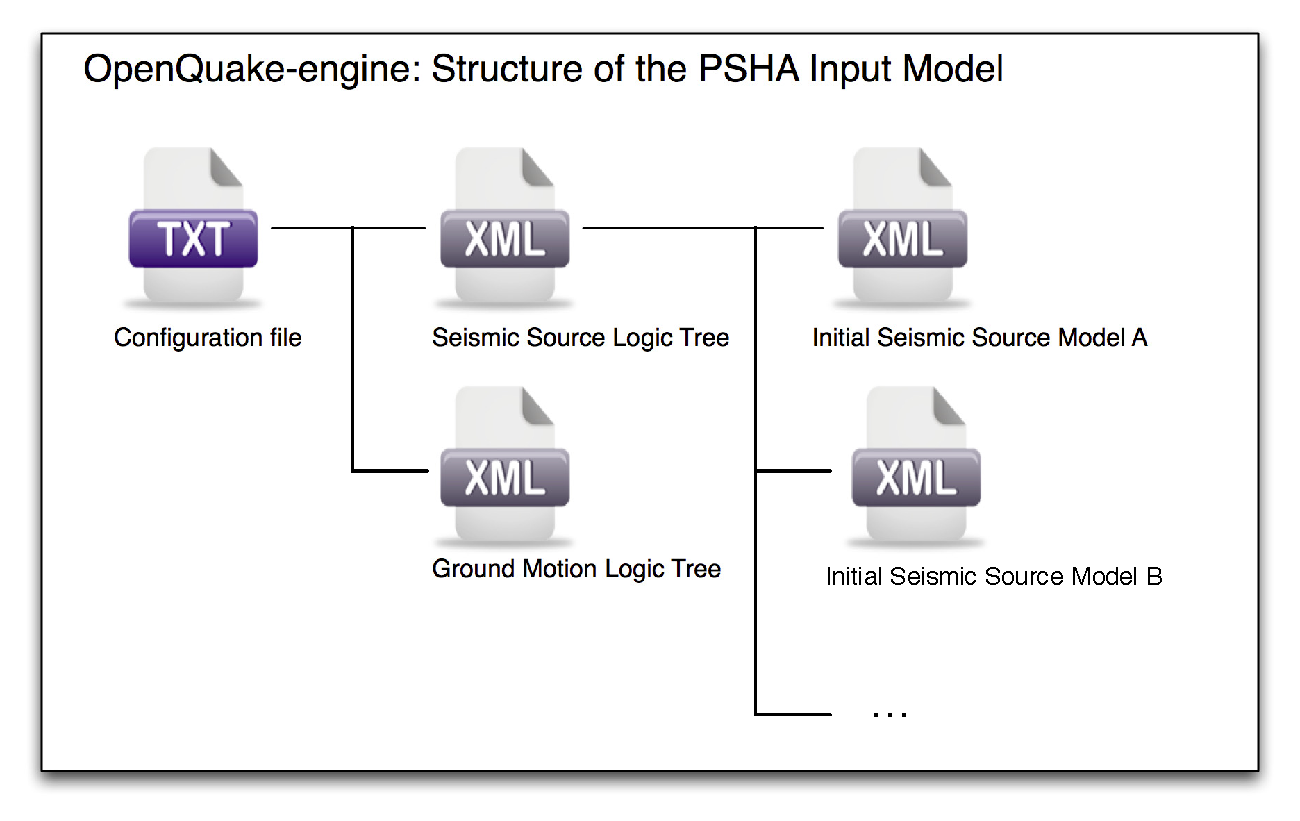
\includegraphics[width=14cm]{figures/hazard/psha_input_structure.pdf}
\caption{PSHA Input Model structure}
\label{fig:psha_input}
\end{figure}


\section{Defining Logic Trees}
The main components of a logic tree structure in the OpenQuake engine are 
the following:
\begin{description}
    \item[branch]: the simplest component of a logic tree structure. 
    A branch represents a possible interpretation/value assignment of 
    a type of uncertainty. It is fully described by the tuple 
    (parameter/model, weight).
    
    \item[branching set]: a key component in the logic tree structure 
    used by the \gls{acr:oqe}. It groups a set of branches i.e. 
    alternative interpretations of a parameter or a model. Each branching
    set is defined by:
    \begin{itemize}
        \item An ID 
        \item An uncertainty type (for a comprehensive list of the types of 
        uncertainty currently supported see Section )
        \item One or more branches
    \end{itemize}
    
    This set of uncertainties can be applied to the whole initial 
    seismic source input model or just to a subset of seismic source
    data. The sum of the weights/probabilities assigned to the set 
    of branches. 

    \item[branching level]: the largest container. It's not used in 
    modelling uncertainty, but it's useful in maintaining a logic and an 
    order in the structure of the tree.
\end{description}

Below we provide a simple schema illustrating the skeleton of the 
\gls{acr:oqe} logic tree:
\begin{Verbatim}[frame=single, commandchars=\\\{\}, fontsize=\small]
\textcolor{green}{<logicTreeBranchingLevel branchingLevelID=ID>}
    \textcolor{blue}{<logicTreeBranchSet branchSetID=ID}
            \textcolor{blue}{uncertaintyType=TYPE>}
        \textcolor{magenta}{<logicTreeBranch>}
            \textcolor{cyan}{<uncertaintyModel>VALUE</uncertaintyModel>}
            \textcolor{cyan}{<uncertaintyWeight>WEIGHT</uncertaintyWeight>}
        \textcolor{magenta}{</logicTreeBranch>}
    \textcolor{blue}{</logicTreeBranchSet>}
\textcolor{green}{</logicTreeBranchingLevel>}
\end{Verbatim}

A schematic representation of these three objects is provided in Figure 
\ref{glts}. A branching level identifies the position in a tree where
branching occurs while a branch set identifies a collection of branches 
(i.e. individual branches) whose weights sum to 1.\\
%
\begin{figure}[!h]
\centering
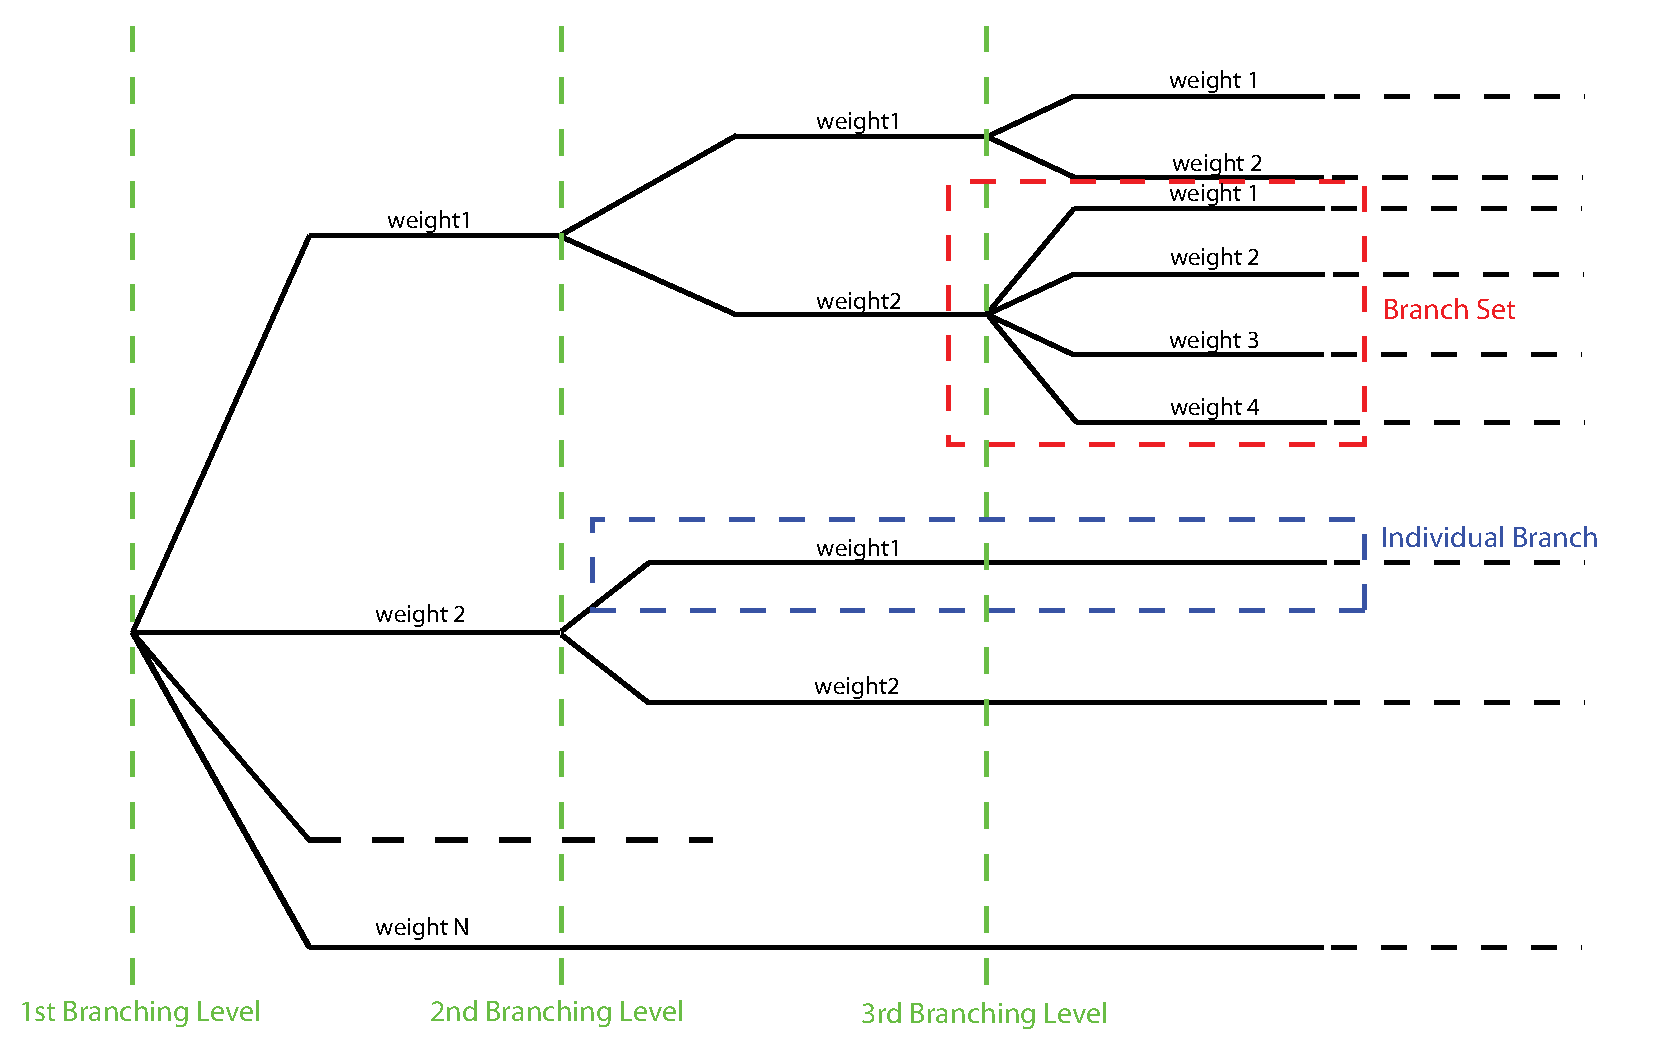
\includegraphics[width=15cm]{./figures/hazard/GenericLogicTreeStructure.eps}
\caption{Generic Logic Tree structure as described in terms of branching 
levels, branch sets, and individual branches.}
\label{glts}
\end{figure}
%
In the NRML schema, a logic tree structure is defined through the 
\Verb+logicTree+ element: 
%
\begin{Verbatim}[frame=single, commandchars=\\\{\}]
<\textcolor{red}{logicTree} logicTreeID="ID">
...
</\textcolor{red}{logicTree}>
\end{Verbatim}
%
A \Verb+logicTree+ contains as a sequence of \Verb+logicTreeBranchingLevel+ 
elements. The position in the sequence specifies in which level of the tree 
the branching level is located. That is, the first 
\texttt{logicTreeBranchingLevel} element in the sequence represents the first 
level in the tree, the second element the second level in the tree, and so on.
%
\begin{Verbatim}[frame=single, commandchars=\\\{\}]
<\textcolor{red}{logicTree} logicTreeID="ID">
	<\textcolor{green}{logicTreeBranchingLevel} branchingLevelID="ID_1">
		...
	</\textcolor{green}{logicTreeBranchingLevel}>
	<\textcolor{green}{logicTreeBranchingLevel} branchingLevelID="ID_2">
		...
	</\textcolor{green}{logicTreeBranchingLevel}>
	....
	<\textcolor{green}{logicTreeBranchingLevel} branchingLevelID="ID_N">
		...
	</\textcolor{green}{logicTreeBranchingLevel}>
</\textcolor{red}{logicTree}>
\end{Verbatim}
No restrictions are present on the number of tree levels that can 
be defined.

A \Verb+logicTreeBranchingLevel+ is defined as a sequence of 
\Verb+logicTreeBranchSet+ elements. Each \Verb+logicTreeBranchSet+ 
defines a particular epistemic uncertainty inside a branching level. 

A branch set has two required attributes (\Verb+branchSetID+ and 
\Verb+uncertaintyType+ (defining the type of epistemic uncertainty 
the branch set is defining))
\begin{Verbatim}[frame=single, commandchars=\\\{\}]
<\textcolor{red}{logicTree} logicTreeID="ID">
...
	<\textcolor{green}{logicTreeBranchingLevel} branchingLevelID="ID_#">
		<\textcolor{blue}{logicTreeBranchSet} branchSetID="ID_1"
			uncertaintyType="UNCERTAINTY_TYPE">
			...
		</\textcolor{blue}{logicTreeBranchSet}>
		<\textcolor{blue}{logicTreeBranchSet} branchSetID="ID_2"
			uncertaintyType="UNCERTAINTY_TYPE">
			...
		</\textcolor{blue}{logicTreeBranchSet}>
		...
		<\textcolor{blue}{logicTreeBranchSet} branchSetID="ID_N"
			uncertaintyType="UNCERTAINTY_TYPE">
			...
		</\textcolor{blue}{logicTreeBranchSet}>
	</\textcolor{green}{logicTreeBranchingLevel}>
...
</\textcolor{red}{logicTree}>
\end{Verbatim}
Possible values for the \Verb+uncertaintyType+ attribute are:
\begin{itemize}
\item \Verb+gmpeModel+: identifying epistemic uncertainties on ground 
motion prediction equations
\item \Verb+sourceModel+: identifying epistemic uncertainties on source models
\item \Verb+maxMagGRRelative+: identifying epistemic uncertainties 
(relative: that is increments) to be added (or subtracted, depending on 
the sign of the increment) to the 
Guten\-berg-Richter maximum magnitude value.
\item \Verb+bGRRelative+: identifying epistemic uncertainties (relative)
to be applied to the Guten\-berg-Richter b value.
\item \Verb+abGRAbsolute+:identifying epistemic uncertainties (absolute: 
that is new values used to replace original values) on the Guten\-berg-Richter
a and b values.
\item \Verb+maxMagGRAbsolute+: identifying epistemic uncertainties 
(absolute) on the Guten\-berg-Richter maximum magnitude.
\end{itemize}
No restrictions are given on the number of branch sets that can be defined 
inside a branching level.

A \Verb+branchSet+ is defined as a sequence of \Verb+logicTreeBranch+ 
elements, each specified by an \Verb+uncertaintyModel+ element (a string 
identifying an uncertainty mod\-el; the content of the string varies with
the uncertaintyType attribute value of the branchSet element) and the
uncertaintyWeight element (specifying the probability/weight associated 
to the uncertaintyModel):
\begin{Verbatim}[frame=single, commandchars=\\\{\}]
<\textcolor{red}{logicTree} logicTreeID="ID">
...
	<\textcolor{green}{logicTreeBranchingLevel} branchingLevelID="ID_#">
		...
		<\textcolor{blue}{logicTreeBranchSet} branchSetID="ID_#"
				uncertaintyType="UNCERTAINTY_TYPE">
			<\textcolor{magenta}{logicTreeBranch} branchID="ID_1">
				<uncertaintyModel>
				UNCERTAINTY_MODEL
				</uncertaintyModel>
				<uncertaintyWeight>
				UNCERTAINTY_WEIGHT
				</uncertaintyWeight>
			</\textcolor{magenta}{logicTreeBranch}>
			...
			<\textcolor{magenta}{logicTreeBranch} branchID="ID_N">
				<uncertaintyModel>
				UNCERTAINTY_MODEL
				</uncertaintyModel>
				<uncertaintyWeight>
				UNCERTAINTY_WEIGHT
				</uncertaintyWeight>
			</\textcolor{magenta}{logicTreeBranch}>
		</\textcolor{blue}{logicTreeBranchSet}>
		...
	</\textcolor{green}{logicTreeBranchingLevel}>
...
</\textcolor{red}{logicTree}>
\end{Verbatim}
Depending on the \Verb+uncertaintyType+ the content of the 
\Verb+<uncertaintyModel>+ element changes:
\begin{itemize}
\item if \Verb+uncertaintyType="gmpeModel"+, the uncertainty model 
contains the name of a ground motion prediction equation (a list of 
available GMPEs are given in appendix A), e.g.:
\begin{Verbatim}[frame=single, commandchars=\\\{\}]
<uncertaintyModel>GMPE_NAME</uncertaintyModel>
\end{Verbatim}
\item if \Verb+uncertaintyType="sourceModel"+, the uncertainty model contains 
the paths to a source model file, e.g.:
\begin{Verbatim}[frame=single, commandchars=\\\{\}]
<uncertaintyModel>SOURCE_MODEL_FILE_PATH</uncertaintyModel>
\end{Verbatim}
\item if \Verb+uncertaintyType="maxMagGRRelative"+, the uncertainty model 
contains the increment to be added (or subtracted, depending on the sign) 
to the Guten\-berg-Richter maximum magnitude:
\begin{Verbatim}[frame=single, commandchars=\\\{\}, samepage=true]
<uncertaintyModel>MAX_MAGNITUDE_INCREMENT</uncertaintyModel>
\end{Verbatim}
\item if \Verb+uncertaintyType="bGRRelative"+, the uncertainty model 
contains the increment to be added (or subtracted, depending on the 
sign) to the Guten\-berg-Richter b value:
\begin{Verbatim}[frame=single, commandchars=\\\{\}, samepage=true]
<uncertaintyModel>B_VALUE_INCREMENT</uncertaintyModel>
\end{Verbatim}
\item if \Verb+uncertaintyType="abGRAbsolute"+, the uncertainty model 
contains one (if the uncertainty apply to a source with only one 
Guten\-berg-Richter magnitude frequency distribution) or more (if the 
source has more than one magnitude frequency distributions) a and b pairs:
\begin{Verbatim}[frame=single, commandchars=\\\{\}, samepage=true]
<uncertaintyModel>
A_VALUE_1 B_VALUE_1
 ... 
A_VALUE_N B_VALUE_N
</uncertaintyModel>
\end{Verbatim}
    \item if \Verb+uncertaintyType="maxMagGRAbsolute"+, the uncertainty 
    model contains one or more (depending on the number of magnitude 
    frequency distributions in the source) Guten\-berg-Richter maximum 
    magnitude values:
%
\begin{Verbatim}[frame=single, commandchars=\\\{\}, samepage=true]
<uncertaintyModel>
MAX_MAGNITUDE_1
 ... 
MAX_MAGNITUDE_N
</uncertaintyModel>
\end{Verbatim}
\end{itemize}
%
No restrictions are given on the number of \Verb+logicTreeBranch+ elements 
that can be defined in a \Verb+logicTreeBranchSet+, as long as the uncertainty 
weights sum to 1.0.

The \Verb+logicTreeBranchSet+ element offers also a number of optional 
attributes allowing for complex tree definitions:
\begin{itemize}
    \item \Verb+applyToBranches+: specifies to which \Verb+logicTreeBranch+ 
    elements (one or more), in the previous branching level, the branch set 
    is linked to. The linking is established by defining the IDs of the 
    branches to link to:
\begin{Verbatim}[frame=single, commandchars=\\\{\}, samepage=true]
applyToBranches="branchID1 branchID2 .... branchIDN"
\end{Verbatim}
    The default is the keyword ALL, which means that a branch set is by default 
    linked to all branches in the previous branching level. By specifying one or 
    more branches to which the branch set links to, non-symmetric logic trees 
    can be defined.
    \item \Verb+applyToSources+: specifies to which source in a source model 
        the uncertainty applies to. Sources are specified in terms of their IDs:
\begin{Verbatim}[frame=single, commandchars=\\\{\}, samepage=true]
applyToSources="srcID1 srcID2 .... srcIDN"
\end{Verbatim}
    \item \Verb+applyToSourceType+: specifies to which source type the 
    uncertainty applies to.  Only one source typology can be defined 
    (\Verb+area+, \Verb+point+, \texttt{simple\-Fault}, 
	\Verb+complexFault+), e.g.:
\begin{Verbatim}[frame=single, commandchars=\\\{\}, samepage=true]
applyToSources="area"
\end{Verbatim}
    \item \Verb+applyToTectonicRegionType+: specifies to which tectonic 
    region type the uncertainty applies to. Only one tectonic region type 
    can be defined (\texttt{Ac\-tive} \texttt{Shallow Crust}, 
    \Verb+Stable Shallow Crust+, \Verb+Subduction Interface+, 
    \texttt{Sub\-duc\-tion} \texttt{IntraSlab}, \texttt{Volcanic}), e.g.:
\begin{Verbatim}[frame=single, commandchars=\\\{\}]
applyToTectonicRegionType="Active Shallow Crust"
\end{Verbatim}
\end{itemize}

\label{sec:hazard_logic_trees}

\section{The Seismic Source System}
The Seismic Source System contains the model (or the models) describing
position, geometry and activity of seismic sources of engineering importance
for a set of sites as well as the possible epistemic uncertainties to be
incorporated into the calculation of seismic hazard.



\subsection{The Seismic Source Logic Tree}

The structure of the Seismic Source Logic Tree consists of at least one
\gls{branchinglevel}. This branching level is the one used to define the
\gls{initialseismicsourceinputmodel} (or a number of initial seismic source
models, see Figure~\ref{fig:psha_input}).

The example provided below shows the simplest Seismic Source Logic Tree
structure that can be defined in a \gls{pshainputmodel} for \gls{acr:oqe}. It's a logic tree with just one branching level containing one \gls{branchset} with one branch used to define the initial seismic source model (its weight will be equal to one). 

\begin{minted}[firstline=1,firstnumber=1,fontsize=\footnotesize,frame=single,bgcolor=lightgray]{xml}
<?xml version="1.0" encoding="UTF-8"?>
<nrml xmlns:gml="http://www.opengis.net/gml"
      xmlns="http://openquake.org/xmlns/nrml/0.5">
    <logicTree logicTreeID="lt1">
        <logicTreeBranchingLevel branchingLevelID="bl1">
            <logicTreeBranchSet uncertaintyType="sourceModel"
                                branchSetID="bs1">
                <logicTreeBranch branchID="b1">
                    <uncertaintyModel>seismic_source_model.xml
                    </uncertaintyModel>
                    <uncertaintyWeight>1.0</uncertaintyWeight>
                </logicTreeBranch>
            </logicTreeBranchSet>
        </logicTreeBranchingLevel>
    </logicTree>
</nrml>
\end{minted}

%\begin{Verbatim}[frame=single, commandchars=\\\{\}, fontsize=\small,
    firstnumber=1, numbers=left, numbersep=2pt]
<?xml version="1.0" encoding="UTF-8"?>
<nrml xmlns:gml="http://www.opengis.net/gml"
      xmlns="http://openquake.org/xmlns/nrml/0.5">
    <logicTree logicTreeID="lt1">
        <logicTreeBranchingLevel branchingLevelID="bl1">
            <logicTreeBranchSet uncertaintyType="sourceModel"
                                branchSetID="bs1">
                <logicTreeBranch branchID="b1">
                    <uncertaintyModel>seismic_source_model.xml
                    </uncertaintyModel>
                    <uncertaintyWeight>1.0</uncertaintyWeight>
                </logicTreeBranch>
            </logicTreeBranchSet>
        </logicTreeBranchingLevel>
    </logicTree>
</nrml>
\end{Verbatim}

The optional branching levels will contain rules that modify parameters of the sources in the initial seismic source model.

For example, if the epistemic uncertainties to be considered are source
geometry and maximum magnitude, the modeller can create a logic tree structure with three initial seismic source models (each one exploring a different definition of the geometry of sources) and one branching level accounting for the epistemic uncertainty on the maximum magnitude.

Below we provide an example of such logic tree structure. Note that the uncertainty on the maximum magnitude is specified in terms of relative increments with respect to the initial maximum magnitude defined for each source in the initial seismic source models.

\inputminted[firstline=1,firstnumber=1,fontsize=\footnotesize,frame=single,linenos,bgcolor=lightgray]{xml}{oqum/hazard/verbatim/input_sslt_simple_lt.xml}
\captionof{listing}{Example source model logic tree structure\label{lst:example_source_model_logic_tree}}

%\begin{Verbatim}[frame=single, commandchars=\\\{\}, fontsize=\small,
    firstnumber=1, numbers=left, numbersep=2pt]
<?xml version="1.0" encoding="UTF-8"?>
<nrml xmlns:gml="http://www.opengis.net/gml"
      xmlns="http://openquake.org/xmlns/nrml/0.5">
    <logicTree logicTreeID="lt1">

        <logicTreeBranchingLevel branchingLevelID="bl1">
            <logicTreeBranchSet uncertaintyType="sourceModel"
                                branchSetID="bs1">
                <logicTreeBranch branchID="b1">
                    <uncertaintyModel>seismic_source_model_A.xml
                    </uncertaintyModel>
                    <uncertaintyWeight>0.2</uncertaintyWeight>
                </logicTreeBranch>
                <logicTreeBranch branchID="b2">
                    <uncertaintyModel>seismic_source_model_B.xml
                    </uncertaintyModel>
                    <uncertaintyWeight>0.3</uncertaintyWeight>
                </logicTreeBranch>
                <logicTreeBranch branchID="b3">
                    <uncertaintyModel>seismic_source_model_C.xml
                    </uncertaintyModel>
                    <uncertaintyWeight>0.5</uncertaintyWeight>
                </logicTreeBranch>
            </logicTreeBranchSet>
        </logicTreeBranchingLevel>

        <logicTreeBranchingLevel branchingLevelID="bl2">
            <logicTreeBranchSet branchSetID="bs21" 
                    uncertaintyType="maxMagGRRelative">
                <logicTreeBranch branchID="b211">
                    <uncertaintyModel>+0.0</uncertaintyModel>
                    <uncertaintyWeight>0.6</uncertaintyWeight>
                </logicTreeBranch>
                <logicTreeBranch branchID="b212">
                    <uncertaintyModel>+0.5</uncertaintyModel>
                    <uncertaintyWeight>0.4</uncertaintyWeight>
                </logicTreeBranch>
            </logicTreeBranchSet>
        </logicTreeBranchingLevel>

    </logicTree>
</nrml>
\end{Verbatim}

\subsection{The Seismic Source Model}
\index{Input!Configuration file}

The structure of the xml file representing the seismic source model
corresponds to a list of sources, each one modelled using one out of the five
typologies currently supported. Below we provide a schematic example of a
seismic source model:

\begin{minted}[firstline=1,firstnumber=1,fontsize=\footnotesize,frame=single,bgcolor=lightgray]{xml}
< sourceModel  gml:id="ID">
	...
	< areaSource  gml:id="SOURCE_ID">
		<gml:name>SOURCE_NAME</gml:name>
		<tectonicRegion>TECT_REGION_TYPE</tectonicRegion>
		...
	</ areaSource >
	...
	< pointSource  gml:id="SOURCE_ID">
		<gml:name>SOURCE_NAME</gml:name>
		<tectonicRegion>TECT_REGION_TYPE</tectonicRegion>
		...
	</ pointSource >
	...
	< simpleFaultSource  gml:id="SOURCE_ID">
		<gml:name>SOURCE_NAME</gml:name>
		<tectonicRegion>TECT_REGION_TYPE</tectonicRegion>
		...
	</ simpleFaultSource >
	...
	< complexFaultSource  gml:id="SOURCE_ID">
		<gml:name>SOURCE_NAME</gml:name>
		<tectonicRegion>TECT_REGION_TYPE</tectonicRegion>
		...
	</ complexFaultSource >
	...
</ sourceModel >
\end{minted}

%\begin{Verbatim}[frame=single, commandchars=\\\{\}, fontsize=\small]
<\textcolor{red}{sourceModel} gml:id="ID">
	...
	<\textcolor{green}{areaSource} gml:id="SOURCE_ID">
		<gml:name>SOURCE_NAME</gml:name>
		<tectonicRegion>TECT_REGION_TYPE</tectonicRegion>
		...
	</\textcolor{green}{areaSource}>
	...
	<\textcolor{green}{pointSource} gml:id="SOURCE_ID">
		<gml:name>SOURCE_NAME</gml:name>
		<tectonicRegion>TECT_REGION_TYPE</tectonicRegion>
		...
	</\textcolor{green}{pointSource}>
	...
	<\textcolor{green}{simpleFaultSource} gml:id="SOURCE_ID">
		<gml:name>SOURCE_NAME</gml:name>
		<tectonicRegion>TECT_REGION_TYPE</tectonicRegion>
		...
	</\textcolor{green}{simpleFaultSource}>
	...
	<\textcolor{green}{complexFaultSource} gml:id="SOURCE_ID">
		<gml:name>SOURCE_NAME</gml:name>
		<tectonicRegion>TECT_REGION_TYPE</tectonicRegion>
		...
	</\textcolor{green}{complexFaultSource}>
	...
</\textcolor{red}{sourceModel}>
\end{Verbatim}

\label{sec:seismic_source_system}

\section{The Ground Motion System}
\index{Input!Ground motion system}
\label{sec:ground_motion_system}
The Ground Motion System defines the models and the possible epistemic
uncertainties related to ground motion modelling to be incorporated into the
calculation.

\subsection{The Ground Motion Logic Tree}
\index{Input!Ground motion logic tree}
\label{subsec:gmlt}

The structure of the \gls{groundmotionlogictree} consists of a list of ground
motion prediction equations for each tectonic region used to characterise the
sources in the PSHA input model.

The example below shows a simple \gls{groundmotionlogictree}. This logic tree
assumes that all the sources in the PSHA input model belong to ``Active
Shallow Crust'' and uses for calculation the \citet{chiou2008}
\gls{acr:gmpe}.

\begin{Verbatim}[frame=single, commandchars=\\\{\}, fontsize=\small,
    firstnumber=1, numbers=left, numbersep=2pt]
<?xml version="1.0" encoding="UTF-8"?>
<nrml xmlns:gml="http://www.opengis.net/gml"
      xmlns="http://openquake.org/xmlns/nrml/0.5">
    <logicTree logicTreeID='lt1'>
        <logicTreeBranchingLevel branchingLevelID="bl1">
            <logicTreeBranchSet uncertaintyType="gmpeModel"
                    branchSetID="bs1"
                    applyToTectonicRegionType="Active Shallow Crust">

                <logicTreeBranch branchID="b1">
                    <uncertaintyModel>
                    ChiouYoungs2008
                    </uncertaintyModel>
                    <uncertaintyWeight>1.0</uncertaintyWeight>
                </logicTreeBranch>

            </logicTreeBranchSet>
        </logicTreeBranchingLevel>
    </logicTree>
</nrml>
\end{Verbatim}


\section{Configuration file}
\index{Input!Configuration file}
\label{sec:hazard_configuration_file}
The configuration file is the primary file controlling both the definition of
the input model as well as parameters governing the calculation. We illustrate
in the following different examples of the configuration file addressing
different typologies of seismic hazard calculation.


\subsection[Classical PSHA]{Classical PSHA}
\label{subsec:config_classical_psha}
In the following we describe the overall structure and the most typical
parameters of a configuration file to be used for the computation of a
seismic hazard map using a classical PSHA methodology.


\textbf{Calculation type and model info}

\begin{minted}[firstline=1,linenos=true,firstnumber=1,fontsize=\footnotesize,frame=single,bgcolor=lightgray]{ini}
[general]
description = A demo OpenQuake-engine .ini file for classical PSHA
calculation_mode = classical
random_seed = 1024
\end{minted}

In this section the user specifies the following parameters:

\begin{itemize}

    \item \texttt{description}: a parameter that can be used to designate
    the model

    \item \texttt{calculation\_mode}: it is used to set the kind of
    calculation. In this case it corresponds to \texttt{classical}.
    Alternative options for the calculation\_mode are described later in this
    manual.

    \item \texttt{random\_seed}: is used to control the random generator
    so that when Monte Carlo procedures are used calculations are
    replicable (if the same \texttt{random\_seed} is used you get exactly
    the same results).

\end{itemize}

\textbf{Geometry of the area (or the sites) where hazard is computed}

This section is used to specify where the hazard will be computed. Two
options are available:

The first ooption is to define a polygon (usually a rectangle) and a distance
(in km) to be used to discretize the  polygon area. The polygon is defined by
a list of longitude-latitude tuples.

An example is provided below:

\begin{minted}[firstline=1,linenos=true,firstnumber=5,fontsize=\footnotesize,frame=single,bgcolor=lightgray]{ini}
[geometry]
region = 10.0 43.0, 12.0 43.0, 12.0 46.0, 10.0 46.0
region_grid_spacing = 10.0
\end{minted}

The second option allows the definition of a number of sites where the hazard
will be computed. An example is provided below:

\begin{minted}[firstline=1,linenos=true,firstnumber=8,fontsize=\footnotesize,frame=single,bgcolor=lightgray]{ini}
[geometry]
sites = 10.0 43.0, 12.0 43.0, 12.0 46.0, 10.0 46.0
\end{minted}

If the list of sites is too long the user can specify the name of a csv file
as shown below:

\begin{minted}[firstline=1,linenos=true,firstnumber=10,fontsize=\footnotesize,frame=single,bgcolor=lightgray]{ini}
[geometry]
sites_csv = <name_of_the_csv_file>
\end{minted}

The format of the csv file containing the list of sites is a sequence of
points (one per row) specified in terms of the longitude, latitude tuple. An
example is provided below:

\begin{minted}[firstline=1,linenos=false,firstnumber=10,fontsize=\footnotesize,frame=single,bgcolor=lightgray]{text}
179.0,90.0
178.0,89.0
177.0,88.0
\end{minted}

\textbf{Logic tree sampling}

The \gls{acr:oqe} provides two options for processing the whole logic tree
structure. The first option uses Montecarlo sampling; the user in this case
specifies a number of realizations.

In the second option all the possible realizations are created. Below we
provide an example for the latter option. In this case we set the
\texttt{number\-\_of\-\_logic\_tree\_samples} to 0. \gls{acr:oqe} will perform
a complete enumeration of all  the possible paths from the roots to the leaves
of the logic tree  structure.

\begin{minted}[firstline=1,linenos=true,firstnumber=12,fontsize=\footnotesize,frame=single,bgcolor=lightgray]{ini}
[logic_tree]
number_of_logic_tree_samples = 0
\end{minted}

If the seismic source logic tree and the ground motion logic tree do not
contain epistemic uncertainties the engine will create a single PSHA input.

\textbf{Generation of the earthquake rupture forecast}

\begin{minted}[firstline=1,linenos=true,firstnumber=14,fontsize=\footnotesize,frame=single,bgcolor=lightgray]{ini}
[erf]
rupture_mesh_spacing = 5
width_of_mfd_bin = 0.1
area_source_discretization = 10
\end{minted}

This section of the configuration file is used to specify the level of
discretization of the mesh representing faults, the grid used to delineate the area sources and, the magnitude-frequency distribution. Note that the smaller is the mesh spacing (or the bin width) the larger are (1) the precision in the calculation and (2) the computation demand.

In cases where the source model may contain a mixture of simple and complex ruptures it is possible to define a different rupture mesh spacing for complex faults only. This may be helpful in models that permit floating ruptures over large subduction sources, in which the nearest source to site distances may be larger than 20 - 30 km, and for which a small mesh spacing would produce a very large number of ruptures. The spacing for complex faults only can be configured by the line:

\begin{minted}[firstline=1,linenos=true,firstnumber=18,fontsize=\footnotesize,frame=single,bgcolor=lightgray]{ini}
comple_rupture_mesh_spacing = 10
\end{minted}

\textbf{Parameters describing site conditions}

\begin{minted}[firstline=1,linenos=true,firstnumber=18,fontsize=\footnotesize,frame=single,bgcolor=lightgray]{ini}
[site_params]
reference_vs30_type = measured
reference_vs30_value = 760.0
reference_depth_to_2pt5km_per_sec = 5.0
reference_depth_to_1pt0km_per_sec = 100.0
\end{minted}

In this section the user specifies local soil conditions. The simplest
solution is to define uniform site conditions (i.e. all the sites have  the
same characteristics).

Alternatively it is possible to define  spatially variable soil properties in
a separate file; the engine will then assign to each investigation location
the values of the closest point used to specify site conditions.

\begin{minted}[firstline=1,linenos=true,firstnumber=23,fontsize=\footnotesize,frame=single,bgcolor=lightgray]{ini}
[site_params]
site_model_file = site_model.xml
\end{minted}

The file containing the site model has the following structure:

\begin{minted}[firstline=1,linenos=false,firstnumber=1,fontsize=\footnotesize,frame=single,bgcolor=lightgray]{xml}
<?xml version="1.0" encoding="utf-8"?>
<nrml xmlns:gml="http://www.opengis.net/gml"
      xmlns="http://openquake.org/xmlns/nrml/0.5">
    <siteModel>
        <site lon="10.0" lat="40.0" vs30="800.0" 
            vs30Type="inferred" z1pt0="19.367196734"
            z2pt5="0.588625072259" backarc="false"/>
        <site lon="10.1" lat="40.0" vs30="800.0" 
            vs30Type="inferred" z1pt0="19.367196734"
            z2pt5="0.588625072259" backarc="false"/>
        <site lon="10.2" lat="40.0" vs30="800.0" 
            vs30Type="inferred" z1pt0="19.367196734"
            z2pt5="0.588625072259" backarc="false"/>
        <site lon="10.3" lat="40.0" vs30="800.0" 
            vs30Type="inferred" z1pt0="19.367196734"
            z2pt5="0.588625072259" backarc="false"/>
        <site lon="10.4" lat="40.0" vs30="800.0" 
            vs30Type="inferred" z1pt0="19.367196734"
            z2pt5="0.588625072259" backarc="false"/>
        ...
    </siteModel>
</nrml>
\end{minted}
%\input{oqum/hazard/verbatim/input_site_model}

If the closest available site with soil conditions is at a distance greater than 5~km from the investigation location, a warning is generated.

\textbf{Calculation configuration}
\phantomsection
\label{sec:calculation_configuration}

\begin{minted}[firstline=1,linenos=true,firstnumber=25,fontsize=\footnotesize,frame=single,bgcolor=lightgray]{ini}
[calculation]
source_model_logic_tree_file = source_model_logic_tree.xml
gsim_logic_tree_file = gmpe_logic_tree.xml
investigation_time = 50.0
intensity_measure_types_and_levels = {"PGA": [0.005, ..., 2.13]}
truncation_level = 3
maximum_distance = 200.0
\end{minted}

This section of the \gls{acr:oqe} configuration file specifies the parameters that are relevant for the calculation of hazard. These include the names of the two files containing the Seismic Source System and the Ground Motion System, the duration of the time window used to compute the  hazard, the ground motion intensity measure types and levels for  which the probability of exceedence will be computed, the level of truncation of the Gaussian distribution of the logarithm of ground motion used in the calculation of hazard and the maximum integration distance (i.e. the distance within which sources will contribute to the computation of the hazard).

The maximum distance refers to the largest distance between a rupture and the target calculation sites in order for the rupture to be considered in the PSHA calculation. This can be input directly in terms of kilometres (as above). There may be cases, however, in which it may be appropriate to have a different maximum source to site distance depending on the tectonic region type. This may be used, for example, to eliminate the impact of small, very far-field sources with very low activity rates in stable tectonic regions (in which case maximum distance is reduced), or conversely it may be raised to allow certain source types to contribute to the hazard at greater distances (such as in the case of large subduction interface events). An example configuration for a maximum distance in Active Shallow Crust of 200 km, and in Stable Continental Crust of 150 km, is shown below:
\begin{minted}[firstline=1,linenos=true,firstnumber=31,fontsize=\footnotesize,frame=single,bgcolor=lightgray]{ini}
maximum_distance = {'Stable Continental Crust': 150.0,
                    'Active Shallow Crust': 200.0}
\end{minted}


\textbf{Output}

\begin{minted}[firstline=1,linenos=true,firstnumber=31,fontsize=\footnotesize,frame=single,bgcolor=lightgray]{ini}
[output]
export_dir = outputs/
# given the specified `intensity_measure_types_and_levels`
mean_hazard_curves = true
quantile_hazard_curves = 0.1 0.5 0.9
uniform_hazard_spectra = false
individual_curves = false
poes = 0.1
\end{minted}

The final section of the configuration file is the one that contains the
parameters controlling the types of output to be produced. Providing an export directory will tell OpenQuake where to place the output files when the \texttt{-{}-exports} flag is used when running the program. Setting \verb=mean_hazard_curves= to true will result in a specific output containing the mean curves of the logic tree, likewise \verb=quantile_hazard_curves= will produce separate files containing the quantile hazard curves at the quantiles listed (0.1, 0.5 and 0.9 in the example above, leave blank or omit if no quantiles are required). Setting \verb=uniform_hazard_spectra= to true will output the uniform hazard spectra at the same probabilities of exceedence (poes) as those specified by the later option \verb=poes=. The probabilities specified here correspond to the set investigation time. 

By default, OpenQuake will export the results for each of the logic tree end branches. If the logic tree contains a large number of end branches the process of exporting the results from each end branch can add a significant amount of computation time - and result in a large volume of disk spaced being used. If instead the user wishes only to export the hazard results for the mean and quantiles then the \verb=individual_curves= option should be set to false. 


\subsection{Seismic hazard disaggregation}
\label{subsec:config_hazard_disaggregation}
In this section we describe the structure of the configuration file to be used
to complete a seismic hazard disaggregation. Since only a few parts of the
standard configuration file need to be changed we can use the description
given in Section~\ref{subsec:config_classical_psha} at
page~\pageref{subsec:config_classical_psha} as a reference and we emphasize
herein major differences.


\begin{minted}[firstline=1,linenos=true,firstnumber=1,fontsize=\footnotesize,frame=single,bgcolor=lightgray]{ini}
[general]
description = A demo .ini file for PSHA disaggregation
calculation_mode = disaggregation
random_seed = 1024
\end{minted}

The calculation mode parameter in this case is set as
\texttt{disaggregation}.



\textbf{Geometry of the area (or the sites) where hazard is computed}

\begin{minted}[firstline=1,linenos=true,firstnumber=5,fontsize=\footnotesize,frame=single,bgcolor=lightgray]{ini}
[geometry]
sites = 11.0 44.5
\end{minted}

In the section it is necessary to specify the geographic coordinates of
the site (or sites) where the disaggregation will be performed.



\textbf{Disaggregation parameters}

\begin{minted}[firstline=1,linenos=true,firstnumber=7,fontsize=\footnotesize,frame=single,bgcolor=lightgray]{ini}
[disaggregation]
poes_disagg = 0.02, 0.1
mag_bin_width = 1.0
distance_bin_width = 25.0
coordinate_bin_width = 1.5
num_epsilon_bins = 3
\end{minted}

With the disaggregation settings shown above we'll disaggregate the intensity
measure levels with 10\% and 2\% probability of exceedance using the
\texttt{in\-ves\-ti\-gation\_time} and the intensity measure types  defined in
the ``Calculation configuration'' section of the OpenQuake configuration file
(see page~\pageref{sec:calculation_configuration}).

The parameters \texttt{mag\_bin\_width},  \texttt{distance\_bin\_width},
\texttt{coordinate\_bin\_width} control the level of discretization of the
disaggregation matrix computed. \texttt{num\_epsilon\_bins} indicates the
number of bins used to represent the contributions provided by different
values of epsilon.

If the user is interested in a specific type of disaggregation, we suggest to
use a very coarse gridding for the parameters that are  not necessary. For
example, if the user is interested in a magnitude-distance  disaggregation, we
suggest the use of very large value for the
\texttt{coordinate\_\-bin\_\-width} and to set  \texttt{num\_epsilon\_bins}
equal to 1.


\subsection{Event based PSHA}
In the following we describe the sections of the configuration file that are
required to complete event based PSHA calculations


\textbf{Calculation type and model info}

This part is almost identical to the corresponding one described in
Section~\ref{subsec:config_classical_psha}. Note the setting of the
\texttt{calculation\_mode} parameter which now corresponds to
\texttt{event\_based}.

\begin{Verbatim}[frame=single, commandchars=\\\{\}, fontsize=\small,
    numbers=left, numbersep=2pt]
[general]
description = A demo OpenQuake-engine .ini file for classical PSHA
calculation_mode = event_based
random_seed = 1024
\end{Verbatim}



\textbf{Event based parameters}

This section is used to specify the number of stochastic event sets to be
generated for each logic tree realisation  (each stochastic event set
represents a potential realisation of seismicity during the
\texttt{investigation\_time} specified in the
\texttt{calculation\_configuration} part). Additionally, in this section the
user can specify the spatial correlation model to be used for the
generation of ground motion fields.

\begin{Verbatim}[frame=single, commandchars=\\\{\}, fontsize=\small]
[event_based_params]
ses_per_logic_tree_path = 5
ground_motion_correlation_model = JB2009
ground_motion_correlation_params = \{"vs30_clustering": True\}
\end{Verbatim}

The acceptable flags for the parameter \verb+vs30_clustering+ are \verb+False+
and \verb+True+, with a capital \verb+F+ and \verb+T+ respectively. \verb+0+
and \verb+1+ are also acceptable flags.



\textbf{Output}

This part substitutes the \texttt{Output} part described in  the configuration
file example described in the Section~ \ref{subsec:config_classical_psha} at
page~\pageref{subsec:config_classical_psha}.

\begin{Verbatim}[frame=single, commandchars=\\\{\}, fontsize=\small]
[output]
export_dir = /tmp/xxx
ground_motion_fields = true
# post-process ground motion fields into hazard curves,
# given the specified `intensity_measure_types_and_levels`
hazard_curves_from_gmfs = true
mean_hazard_curves = true
quantile_hazard_curves = 0.15 0.5 0.85
poes = 0.1 0.2
\end{Verbatim}

The option \verb=hazard_curves_from_gmfs= instructs the user to use the event-based ground motion values to provide hazard curves indicating the probabilities of exceeding the intensity measure levels set previously in the \verb=intensity_measure_types_and_levels= option.

\label{subsec:config_event_based_psha}

   \cleardoublepage

\chapterimage{figures/chapter_head.pdf} % Chapter heading image
\chapter{Hazard Calculations and Results}
	\label{chap:hazoutputs}
	In this Chapter we provide a desciption of the main commands available for
running hazard with the \gls{acr:oqe} and the file formats used to represent
the results of the analyses.

A general introduction on the use of the \glsdesc{acr:oqe} is provided in
Section~\ref{sec:running_oq_engine} at page~\pageref{sec:running_oq_engine}. The
reader is invited to consult this part before diving into the following
sections.


% -----------------------------------------------------------------------------
\section{Running OpenQuake-engine for hazard calculations}
\label{sec:running_hazard_calculations}
\index{Running OpenQuake!hazard}

The execution of a hazard analysis using the OpenQuake-engine is
straightforward. Below we provide an example of the simplest command that can be
used to launch a hazard calculation. It consists in the invocation of \texttt
{oq-engine} together with the \texttt{-{}-run} or \texttt{-{}-rh} (run-hazard) option, and the name of a configuration file (in the example below it
corresponds to \texttt{job.ini}):

\begin{Verbatim}[frame=single, commandchars=\\\{\}, fontsize=\small]
user@ubuntu:~$ oq engine --run job.ini
\end{Verbatim}

The amount of information prompted during the execution of the analysis can be
controlled through the \texttt{-{}-log-level} flag as shown in the example below:

\begin{Verbatim}[frame=single, commandchars=\\\{\}, fontsize=\small]
user@ubuntu:~$ oq engine --rh job.ini --log-level debug
\end{Verbatim}

In this example we ask the engine to provide an extensive amount of information
(usually not justified for a standard analysis). Alternative options are:
\texttt{debug}, \texttt{info}, \texttt{progress}, \texttt{warn}, \texttt{error},
\texttt{critical}.


% -----------------------------------------------------------------------------
\section{Exporting results from a hazard calculation}
\label{sec:exporting_hazard_results}

There are two alternative ways to get results from the OpenQuake-engine:
directly through the calculation or by exporting them from the internal
\gls{acr:oqe} database once a calculation is completed.

The first option is defined at the OpenQuake-engine invocation through the
flag \texttt{--exports xml}, as shown in the example below:

\begin{Verbatim}[frame=single, commandchars=\\\{\}, fontsize=\small]
user@ubuntu:~$ oq engine --run job.ini \textcolor{red}{--exports xml}
\end{Verbatim}
\noindent This will export the results to the \verb=results= directory specified in the \verb=job.ini= file. 

The second option allows the user to export the computed results or just a
subset of them whenever they want. In order to obtain the list of results of
the hazard calculations stored in the \gls{acr:oqe} database the user can
utilize the \texttt{-{}-lhc} command (`list hazard calculations') to list the hazard calculations:

\begin{Verbatim}[frame=single, commandchars=\\\{\}, fontsize=\small]
user@ubuntu:~$ oq engine --lhc
\end{Verbatim}

The execution of this command will produce a list similar to the one provided
below (the numbers in red are the calculations IDs):

\begin{Verbatim}[frame=single, commandchars=\\\{\}, fontsize=\small]
user@ubuntu:~$ oq engine --lhc
job_id | status | start_time | description
\textcolor{red}{1} | failed | 2013-03-01 09:49:34 | Classical PSHA
\textcolor{red}{2} | successful | 2013-03-01 09:49:56 | Classical PSHA
\textcolor{red}{3} | failed | 2013-03-01 10:24:04 | Classical PSHA
\textcolor{red}{4} | failed | 2013-03-01 10:28:16 | Classical PSHA
\textcolor{red}{5} | failed | 2013-03-01 10:30:04 | Classical PSHA
\textcolor{red}{6} | successful | 2013-03-01 10:31:53 | Classical PSHA
\textcolor{red}{7} | failed | 2013-03-09 08:15:14 | Classical PSHA
\textcolor{red}{8} | successful | 2013-03-09 08:18:04 | Classical PSHA
\end{Verbatim}

Subsequently the user can get the list of result stored for a specific hazard
analysis by using the \texttt{-{}-list-outputs}, or \texttt{-{}-lo}, command, as in the example below (note that the number in blue emphasizes the
result ID):

\begin{Verbatim}[frame=single, commandchars=\\\{\}, fontsize=\small]
user@ubuntu:~$ oq engine --lo <calc_id>
id | output_type | name
\textcolor{blue}{3} | datastore | hcurves
\end{Verbatim}

and finally extract an xml file for a specific hazard result:

\begin{Verbatim}[frame=single, commandchars=\\\{\}, fontsize=\small]
user@ubuntu:~$ oq engine --export-outputs <result_id> <output_folder>
\end{Verbatim}


% -----------------------------------------------------------------------------
\section{Description of hazard outputs}
\label{sec:hazard_outputs}

The results generated by the OpenQuake-engine are fundamentally of two
distinct typologies differentiated by the presence (or absence) of epistemic
uncertainty in the PSHA input model.

When epistemic uncertainty is incorporated into the calculation, the
OpenQuake-engine calculators (e.g. Classical PSHA, Event Based PSHA,
Disaggregation, UHS) produce a set of results (i.e. hazard curves, ground
motion fields, disaggregation matrices, UHS, for each logic-tree realisation)
which reflects epistemic uncertainties introduced in the PSHA input model. The user can specify that only the mean results and desired quantiles are exported by using the optional configuration \verb+individual_curves=False+ in the \verb=job.ini= file.

For each logic tree sample, results are computed and stored. Calculation of
results statistics (mean, standard deviation, quantiles) are supported by all
the calculators, with the exception of the disaggregation calculator.

\subsection{Outputs from Classical PSHA}
\label{subsec:output_classical_psha}
By default, the classical PSHA calculator computes and stores hazard curves
for each logic tree sample considered.

When the PSHA input model doesn't contain epistemic uncertainties the results
is a set of hazard curves (one for each investigated site). The command below
illustrates how is possible to retrieve the group of hazard curves obtained
for a calculation with a given identifier \texttt{<calc\_id>} (see
Section~\ref{sec:exporting_hazard_results} for an explanation about how to
obtain the list of calculations performed with their corresponding ID):

\begin{Verbatim}[frame=single, commandchars=\\\{\}, fontsize=\small]
user@ubuntu:~$ oq-engine --lo <calc_id>
id | output_type | name
\textcolor{red}{3 | hazard_curve | hc-rlz-6}
\end{Verbatim}

In this case the \gls{acr:oqe} computed a group of hazard curves with result
ID equal to \texttt{3}. On the contrary, if the parameter
\texttt{number\_of\_logic\_tree\_samples} in the configuration file is
different than zero, then N hazard curves files are generated. The example
below shows this case:

\begin{Verbatim}[frame=single, commandchars=\\\{\}, fontsize=\small]
user@ubuntu:~$ oq engine --lo <calc_id>
id | output_type | name
\textcolor{red}{5 | datastore | hcurves}
\textcolor{red}{6 | datastore | hcurves}
\textcolor{red}{7 | datastore | hcurves}
\textcolor{red}{8 | datastore | hcurves}
\textcolor{red}{9 | datastore | hcurves}
\textcolor{red}{10 | datastore | hcurves}
\end{Verbatim}

If we export from the database the hazard curves contained in one of the
items above using the following command:

\begin{Verbatim}[frame=single, commandchars=\\\{\}, fontsize=\small]
user@ubuntu:~$ oq-engine --export-outputs <output_id> <output_directory>
\end{Verbatim}

we obtain a nrml formatted file as represented in the example in the inset
below:

\begin{Verbatim}[frame=single, commandchars=\\\{\}, fontsize=\small]
<?xml version='1.0' encoding='UTF-8'?>
<nrml xmlns:gml="http://www.opengis.net/gml"
      xmlns="http://openquake.org/xmlns/nrml/0.5">
  <hazardCurves \textcolor{red}{sourceModelTreePath="b1|b212"}
      \textcolor{red}{gsimTreePath="b2" IMT="PGA" investigationTime="50.0"}>
    \textcolor{green}{<IMLs>0.005 0.007 0.0098 ... 1.09 1.52 2.13</IMLs>}
    <hazardCurve>
      <gml:Point>
      \textcolor{blue}{<gml:pos>10.0 45.0</gml:pos>}
      </gml:Point>
      <poEs>1.0 1.0 1.0 ... 0.000688359310522 0.0 0.0</poEs>
    </hazardCurve>
    ...
    <hazardCurve>
      <gml:Point>
      \textcolor{blue}{<gml:pos>lon lat</gml:pos>}
      </gml:Point>
      <poEs>poe1 poe2 ... poeN</poEs>
    </hazardCurve>
  </hazardCurves>
</nrml>
\end{Verbatim}

Notwithstanding the intuitiveness of this file, let's have a brief
overview of the information included.

The overall content of this file is a list of hazard curves, one for each
investigated site, computed using a PSHA input model representing one possible
realisation obtained using the complete logic tree structure.

The attributes of the \texttt{hazardCurves} element (see text in red) specify
the path of the logic tree used to create the seismic source model
(\texttt{source\-Model\-TreePath}) and the ground motion model
(\texttt{gsim\-Tree\-Path}) plus the intensity measure type and the
investigation time used to compute the probability of exceedance.

The \texttt{IMLs} element (in green in the example) contains the values of
shaking used by the engine to compute the probability of exceedance in the
investigation time. For each site this file contains a \texttt{hazardCurve}
element which has the coordinates (longitude and latitude in decimal degrees)
of the site and the values of the probability of exceedance for all the
intensity measure levels specified in the \texttt{IMLs} element.

If in the configuration file the calculation of mean hazard curves and hazard
curves corresponding to one or several percentiles have been specified, the
list of outputs that we should expect from the \glsdesc{acr:oqe} corresponds
to:

\begin{Verbatim}[frame=single, commandchars=\\\{\}, fontsize=\small]
user@ubuntu:~$ oq-engine --lho <calc_id>
id | output_type | name
17 | hazard_curve | hc-rlz-17
18 | hazard_curve | hc-rlz-18
19 | hazard_curve | hc-rlz-13
20 | hazard_curve | hc-rlz-14
21 | hazard_curve | hc-rlz-15
22 | hazard_curve | hc-rlz-16
\textcolor{red}{23 | hazard_curve | quantile(0.5)-curves-PGA}
24 | hazard_map | hazard-map(0.1)-PGA-rlz-17
25 | hazard_map | hazard-map(0.1)-PGA-rlz-18
26 | hazard_map | hazard-map(0.1)-PGA-rlz-13
27 | hazard_map | hazard-map(0.1)-PGA-rlz-14
28 | hazard_map | hazard-map(0.1)-PGA-rlz-15
29 | hazard_map | hazard-map(0.1)-PGA-rlz-16
\textcolor{red}{30 | hazard_map | hazard-map(0.1)-PGA-quantile(0.5)}
\end{Verbatim}

In this example the \gls{acr:oqe} produced hazard curves and hazard maps for
six logic tree realisations plus median hazard curves and the median hazard
map (both highlighted in red).

The following inset shows a sample of the nrml file used to describe a hazard
map:

\begin{Verbatim}[frame=single, commandchars=\\\{\}, fontsize=\small]
<?xml version='1.0' encoding='UTF-8'?>
<nrml xmlns:gml="http://www.opengis.net/gml"
      xmlns="http://openquake.org/xmlns/nrml/0.4">
  \textcolor{red}{<hazardMap sourceModelTreePath="b1" gsimTreePath="b1"}
        \textcolor{red}{IMT="PGA" investigationTime="50.0" poE="0.1">}
    <node lon="119.596690957" lat="21.5497682591" iml="0.204569990197"/>
    <node lon="119.596751048" lat="21.6397004197" iml="0.212391638188"/>
    <node lon="119.596811453" lat="21.7296325803" iml="0.221407505615"/>
    ...
  </hazardMap>
</nrml>
\end{Verbatim}

\subsection{Outputs from Hazard Disaggregation}
\label{subsec:output_hazard_disaggregation}
\section{Output from Disaggregation}
The output from an \gls{acr:oqe} disaggregation analysis  
correspond to the combination of a hazard curve and a multidimensional 
matrix containing the results of the disaggregation.

The example below shows the list of disaggregation results obtained 
for four logic tree realisations. 
For each realisation, disaggregation has been completed for two  
intensity measure levels corresponding to different probabilities of 
exceedence in the specified \texttt{investigation time}.
\begin{Verbatim}[frame=single, commandchars=\\\{\}, samepage=true]
user@ubuntu:~$ openquake --lho <calc_id> 
id | output_type | name
19 | hazard_curve | hc-rlz-3
20 | hazard_curve | hc-rlz-3
21 | hazard_curve | hc-rlz-4
22 | hazard_curve | hc-rlz-4
23 | disagg_matrix | disagg(0.02)-rlz-3-SA(0.025)-POINT(10.1 40.1)
24 | disagg_matrix | disagg(0.1)-rlz-3-SA(0.025)-POINT(10.1 40.1)
25 | disagg_matrix | disagg(0.02)-rlz-3-PGA-POINT(10.1 40.1)
26 | disagg_matrix | disagg(0.1)-rlz-3-PGA-POINT(10.1 40.1)
27 | disagg_matrix | disagg(0.02)-rlz-4-SA(0.025)-POINT(10.1 40.1)
28 | disagg_matrix | disagg(0.1)-rlz-4-SA(0.025)-POINT(10.1 40.1)
29 | disagg_matrix | disagg(0.02)-rlz-4-PGA-POINT(10.1 40.1)
30 | disagg_matrix | disagg(0.1)-rlz-4-PGA-POINT(10.1 40.1)
\end{Verbatim}

In the following (see Inset \ref{vrb:disaggr}) we show 
%\begin{nrmlsmp}
\begin{Verbatim}[frame=single, commandchars=\\\{\}, fontsize=\small]
<?xml version='2.0' encoding='UTF-8'?>
<nrml xmlns:gml="http://www.opengis.net/gml" 
      xmlns="http://openquake.org/xmlns/nrml/0.4">
  <disaggMatrices sourceModelTreePath="b1" gsimTreePath="b1" IMT="PGA" 
        investigationTime="50.0" lon="10.1" lat="40.1" 
        magBinEdges="5.0, 6.0, 7.0, 8.0" 
        distBinEdges="0.0, 25.0, 50.0, 75.0, 100.0" 
        lonBinEdges="9.0, 10.5, 12.0" 
        latBinEdges="39.0, 40.5" 
        epsBinEdges="-3.0, -1.0, 1.0, 3.0" 
        tectonicRegionTypes="Active Shallow Crust">
    <disaggMatrix type="Mag" dims="3" poE="0.1" iml="0.033424622602">
    <disaggMatrix type="Mag" dims="3" poE="0.1" iml="0.033424622602">
      <prob index="0" value="0.987374744394"/>
      <prob index="1" value="0.704295394366"/>
      <prob index="2" value="0.0802318409498"/>
    </disaggMatrix>
    <disaggMatrix type="Dist" dims="4" poE="0.1" iml="0.033424622602">
      <prob index="0" value="0.700851969171"/>
      <prob index="1" value="0.936680387051"/>
      <prob index="2" value="0.761883595568"/>
      <prob index="3" value="0.238687565571"/>
    </disaggMatrix>
    <disaggMatrix type="TRT" dims="1" poE="0.1" iml="0.033424622602">
      <prob index="0" value="0.996566187011"/>
    </disaggMatrix>
    <disaggMatrix type="Mag,Dist" dims="3,4" poE="0.1" iml="0.033424622602">
      <prob index="2,3" value="0.0"/>
    </disaggMatrix>
    <disaggMatrix type="Mag,Dist,Eps" dims="3,4,3" poE="0.1" iml="0.033424622602">
      <prob index="0,0,0" value="0.0785857271425"/>
\end{Verbatim}
%\caption{Hazard map: nrml sample file}
%\label{vrb:disaggr}
%\end{nrmlsmp}



\subsection{Outputs from Event Based PSHA}
\label{subsec:output_event_based_psha}
\section{Output from Event Based PSHA}\label{EventBasedOutput}
%
The Event Based PSHA calculator computes and stores stochastic 
event sets and the corresponding ground motion fields. In case,
this calculator can also compute hazard curves and hazard maps
exactly in the same way is done using the Classical PSHA calculator.

The inset below shows an example of the list of results provided by 
\gls{acr:oqe} at the end of an event-based PSHA calculation:
%
\begin{Verbatim}[frame=single, commandchars=\\\{\}, fontsize=\small]
user@ubuntu:~$ oq-engine --lho <calc_id> 
id | output_type | name
\textcolor{red}{31 | ses | ses-coll-rlz-19}
\textcolor{green}{32 | gmf | gmf-rlz-19}
\textcolor{red}{33 | ses | ses-coll-rlz-20}
\textcolor{green}{34 | gmf | gmf-rlz-20}
35 | hazard_curve | hazard-curve-rlz-19-SA(0.1)
36 | hazard_curve | hazard-curve-rlz-20-SA(0.1)
37 | hazard_curve | hazard-curve-rlz-19-PGA
38 | hazard_curve | hazard-curve-rlz-20-PGA
39 | hazard_curve | mean curve for SA(0.1)
40 | hazard_curve | quantile curve (poe >= 0.15) for imt SA(0.1)
41 | hazard_curve | quantile curve (poe >= 0.5) for imt SA(0.1)
42 | hazard_curve | quantile curve (poe >= 0.85) for imt SA(0.1)
43 | hazard_curve | mean curve for PGA
44 | hazard_curve | quantile curve (poe >= 0.15) for imt PGA
45 | hazard_curve | quantile curve (poe >= 0.5) for imt PGA
46 | hazard_curve | quantile curve (poe >= 0.85) for imt PGA
\end{Verbatim}
This list contains two sets of stochastic events (in red) two sets of ground motion fields (in blue).

The whole group of stochastic event set and ground motion fields can 
be exported immediately using the results with \texttt{id} 35 and 25,
respectively.

In the remaining part of this Section we show an example of a file
containing a stochastic event set and a file containing a ground 
motion field.

This is an example showing a nrml file containing two a collection of 
stochastic event sets 
\begin{Verbatim}[frame=single, commandchars=\\\{\}, fontsize=\small]
<?xml version='1.0' encoding='UTF-8'?>
<nrml xmlns:gml="http://www.opengis.net/gml" 
	  xmlns="http://openquake.org/xmlns/nrml/0.4">
  <stochasticEventSetCollection sourceModelTreePath="b1" 
          gsimTreePath="b1">
    \textcolor{red}{<stochasticEventSet id="12" investigationTime="50.0">}
      <rupture id="533" magnitude="4.55" strike="90.0" dip="90.0" 
              rake="90.0" tectonicRegion="Active Shallow Crust">
        <planarSurface>
          <topLeft lon="12.233903801" lat="43.256198599" 
                  depth="11.3933265259"/>
          <topRight lon="12.263958243" lat="43.2562025344" 
                  depth="11.3933265259"/>
          <bottomLeft lon="12.233903801" lat="43.256198599" 
                  depth="12.6066734741"/>
          <bottomRight lon="12.263958243" lat="43.2562025344" 
                  depth="12.6066734741"/>
        </planarSurface>
      </rupture>
      <rupture id="535" magnitude="4.65" strike="135.0" dip="90.0" 
              rake="90.0" tectonicRegion="Active Shallow Crust">
        <planarSurface>
          <topLeft lon="11.45858812" lat="42.7429056814" 
                  depth="11.3208667302"/>
          <topRight lon="11.4822820715" lat="42.7256333907" 
                  depth="11.3208667302"/>
          <bottomLeft lon="11.45858812" lat="42.7429056814" 
                  depth="12.6791332698"/>
          <bottomRight lon="11.4822820715" lat="42.7256333907" 
                  depth="12.6791332698"/>
        </planarSurface>
      </rupture>
    \textcolor{red}{</stochasticEventSet>}
  </stochasticEventSetCollection>
</nrml>
\end{Verbatim}
This is an example showing a nrml file containing a collection of
ground motion fields:
\begin{Verbatim}[frame=single, commandchars=\\\{\}, fontsize=\small]
<?xml version='1.0' encoding='UTF-8'?>
<nrml xmlns:gml="http://www.opengis.net/gml" 
      xmlns="http://openquake.org/xmlns/nrml/0.4">
  <gmfCollection sourceModelTreePath="b1" gsimTreePath="b1">
    <gmfSet investigationTime="50.0" stochasticEventSetId="12">
      <gmf IMT="PGA" ruptureId="533">
        <node gmv="0.0105891230432" lon="11.1240023202" 
            lat="43.5107462335"/>
        <node gmv="0.00905803920023" lon="11.1241875202" 
            lat="43.6006783941"/>
        <node gmv="0.00637664420977" lon="11.124373581" 
            lat="43.6906105547"/>
        <node gmv="0.00476533134789" lon="11.1245605075" 
            lat="43.7805427153"/>
        <node gmv="0.00452594698469" lon="11.1247483046" 
            lat="43.8704748759"/>
        ...
        <node gmv="0.000173010769646" lon="11.3782630185" 
            lat="44.5"/>
      </gmf>
    </gmfSet>
  </gmfCollection>
</nrml>
\end{Verbatim}


   \cleardoublepage

\chapterimage{figures/chapter_head.pdf} % Chapter heading image
\chapter{Demonstrative Examples}
	\label{chap:hazdemos}
	% -----------------------------------------------------------------------------
\section{OpenQuake Hazard Demos}
Together with the \gls{acr:oqe} installation a number of demos are provided 
showing different examples of input and configuration files, for different 
use cases.

This is the list of demos which illustrate how to use the \gls{acr:oqe} for 
various seismic hazard analysis:
\begin{itemize}
\item AreaSourceClassicalPSHA
\item CharacteristicFaultSourceCase1ClassicalPSHA
\item CharacteristicFaultSourceCase2ClassicalPSHA
\item CharacteristicFaultSourceCase3ClassicalPSHA
\item ComplexFaultSourceClassicalPSHA
\item Disaggregation
\item EventBasedPSHA
\item LogicTreeCase1ClassicalPSHA
\item LogicTreeCase2ClassicalPSHA
\item LogicTreeCase3ClassicalPSHA
\item PointSourceClassicalPSHA
\item SimpleFaultSourceClassicalPSHA
\end{itemize}

\subsection{Classical PSHA Demos}
A number of demos have been designed to show how to perform a classical PSHA 
calculation using the different available
source typologies and how to define non-trivial logic trees. It should be 
noted that the input files that will be illustrated are valid
not only for a classical PSHA calculation but also for event based and 
disaggregation analysis.

All the classical PSHA demos illustrating the different source typologies 
(all demos but the ones about Logic Tree definition)
share the same GSIM logic tree file, which for clarity is 
provided below.

Since this logic tree consideres only one tectonic region (i.e.
\texttt{Active Shallow Crust}) all the seismic sources will belong
be considered active shallow crust sources.

\begin{Verbatim}[frame=single, commandchars=\\\{\}, fontsize=\normalsize]
<?xml version="1.0" encoding="UTF-8"?>

<nrml xmlns:gml="http://www.opengis.net/gml"
      xmlns="http://openquake.org/xmlns/nrml/0.4">
    <logicTree logicTreeID='lt1'>

        <logicTreeBranchingLevel branchingLevelID="bl1">
            <logicTreeBranchSet
               uncertaintyType="gmpeModel"
               applyToTectonicRegionType="Active Shallow Crust"
               branchSetID="bs1">

                <logicTreeBranch branchID="b1">
                     <uncertaintyModel>
                        BooreAtkinson2008
                     </uncertaintyModel>
                     <uncertaintyWeight>1.0</uncertaintyWeight>
                </logicTreeBranch>

            </logicTreeBranchSet>
        </logicTreeBranchingLevel>

    </logicTree>
</nrml>
\end{Verbatim}

\subsubsection{Classical PSHA with different source typologies}

This section discusses the following examples:
\begin{itemize}
\item AreaSourceClassicalPSHA
\item CharacteristicFaultSourceCase1ClassicalPSHA
\item CharacteristicFaultSourceCase2ClassicalPSHA
\item CharacteristicFaultSourceCase3ClassicalPSHA
\item ComplexFaultSourceClassicalPSHA
\item PointSourceClassicalPSHA
\item SimpleFaultSourceClassicalPSHA
\end{itemize}

The configuration file (see below) is defined to compute hazard 
curves for several intensity measure types (PGV, PGA and Spectral
acceleration at different periods), hazard maps and uniform hazard 
spectra for different probabilities of exceedance:
\begin{Verbatim}[frame=single, commandchars=\\\{\}, fontsize=\normalsize]
[general]

description = ...
calculation_mode = classical
random_seed = 23

[geometry]

region = ...
region_grid_spacing = 5.0

[logic_tree]

number_of_logic_tree_samples = 0

[erf]

rupture_mesh_spacing = 2
width_of_mfd_bin = 0.1
area_source_discretization = 5.0

[site_params]

reference_vs30_type = measured
reference_vs30_value = 600.0
reference_depth_to_2pt5km_per_sec = 5.0
reference_depth_to_1pt0km_per_sec = 100.0

[calculation]

source_model_logic_tree_file = source_model_logic_tree.xml
gsim_logic_tree_file = gmpe_logic_tree.xml
investigation_time = 50.0
intensity_measure_types_and_levels =\{
"PGV": [2, 4, 6 ,8, 10, ...], 
"PGA": [0.005, 0.007, ...], 
"SA(0.025)": [...], 
"SA(0.05)": [...],
"SA(0.1)": [...], 
"SA(0.2)": [...], 
"SA(0.5)": [...], 
"SA(1.0)": [...],
"SA(2.0)": [...]\}
truncation_level = 3
maximum_distance = 200.0

[output]

export_dir = ...
mean_hazard_curves = false
quantile_hazard_curves =
hazard_maps = true
uniform_hazard_spectra = true
poes = 0.1 0.02
\end{Verbatim}
Hazard maps for the different demos are show in figure 
\ref{fig:hazard_maps1} and \ref{fig:hazard_maps2}.

\begin{figure} 
\centering 
\subcaptionbox{}
{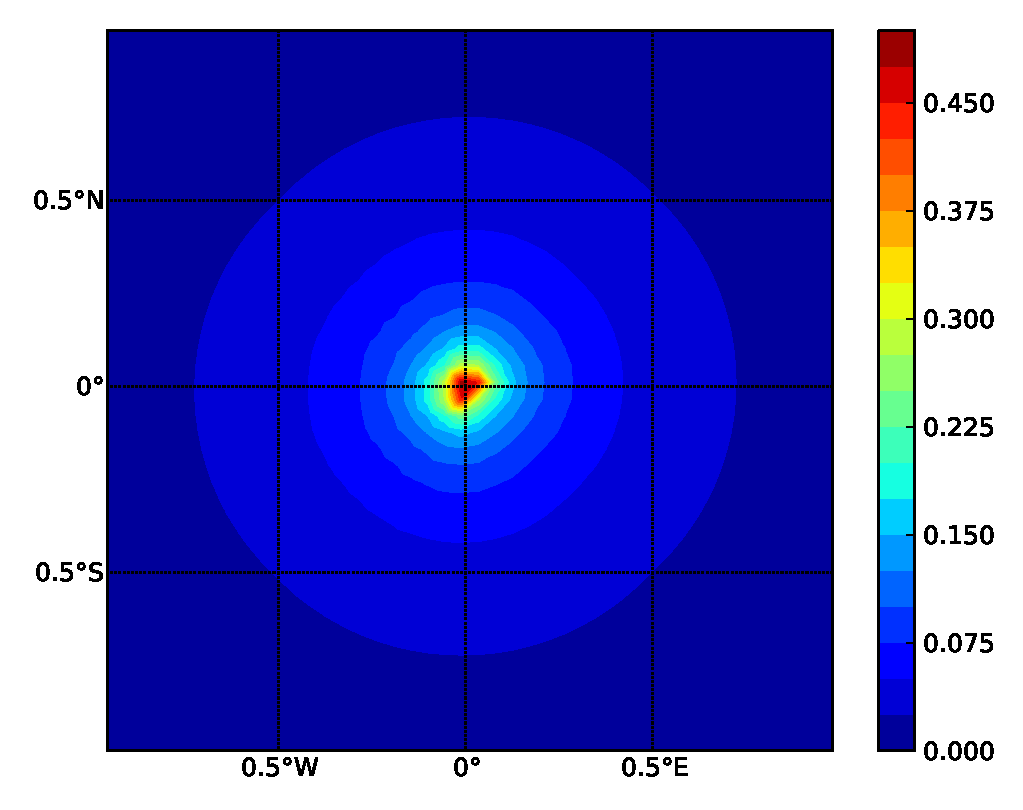
\includegraphics[width=7cm]{./figures/hazard/point.eps}} 
\subcaptionbox{}
{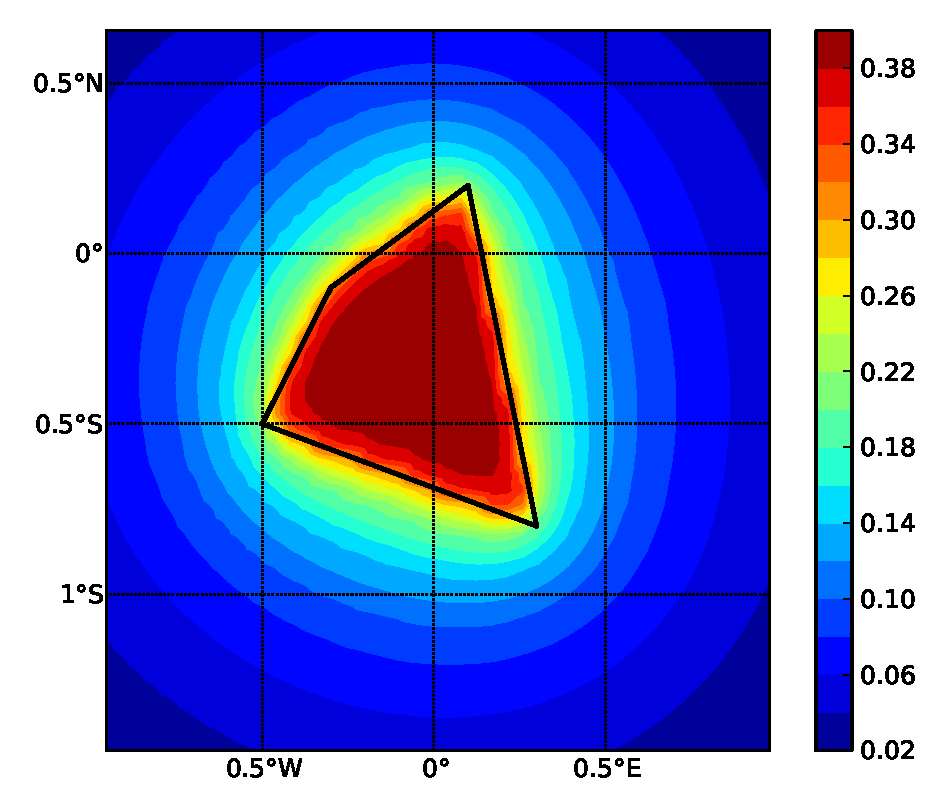
\includegraphics[width=7cm]{./figures/hazard/area.eps}} 
\subcaptionbox{}
{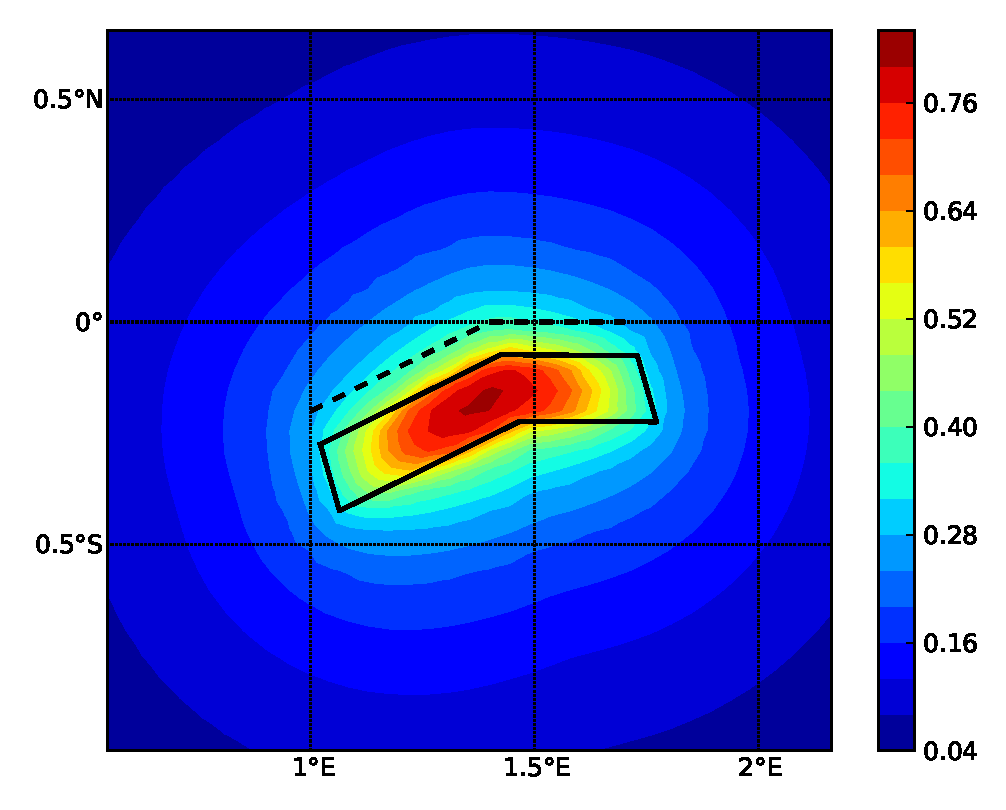
\includegraphics[width=7cm]{./figures/hazard/simple_fault.eps}} 
\subcaptionbox{}
{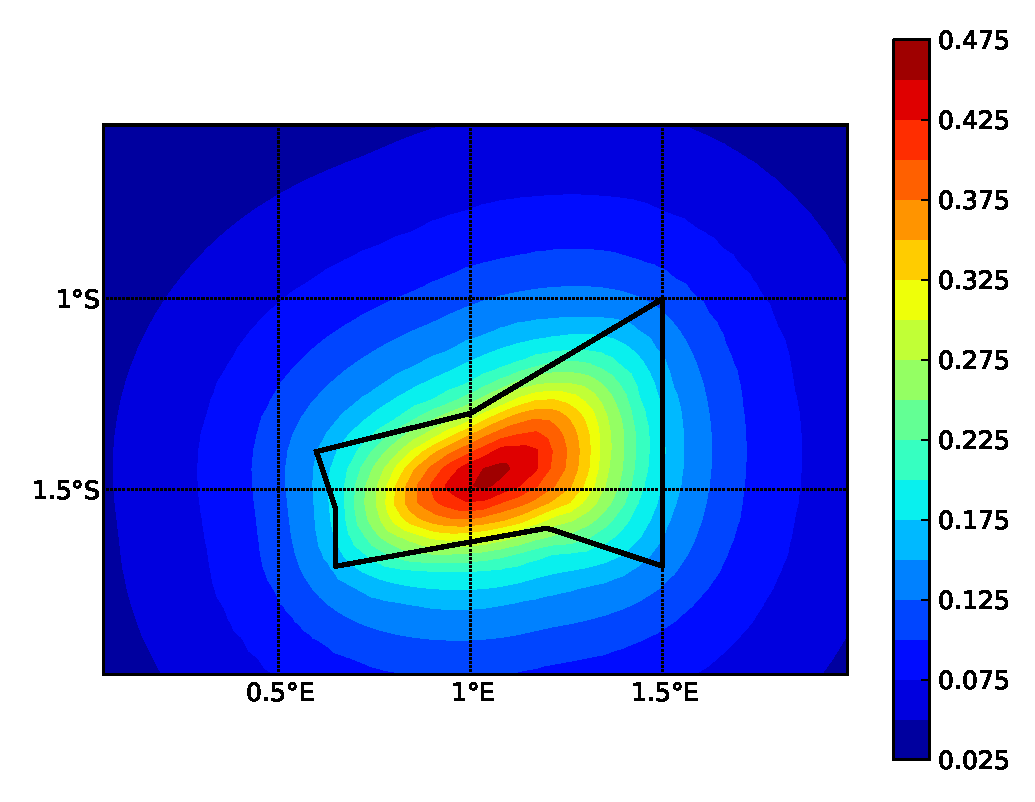
\includegraphics[width=7cm]{./figures/hazard/complex_fault.eps}} 
\caption{Hazard maps (for PGA, 10\% in 50 years) as obtained from the 
    different \gls{acr:oqe} source typologies. (a) Point Source. (b) Area 
    source.  The solid black line represents the area boundary. (c) Simple 
    Fault Source. 
    The dashed line represents the fault trace, while the solid line the fault
    surface projection. (d) Complex Fault Source. The solid line represent the 
    fault surface projection (d)}
\label{fig:hazard_maps1}
\end{figure}

\begin{figure} 
\centering 
\subcaptionbox{}
{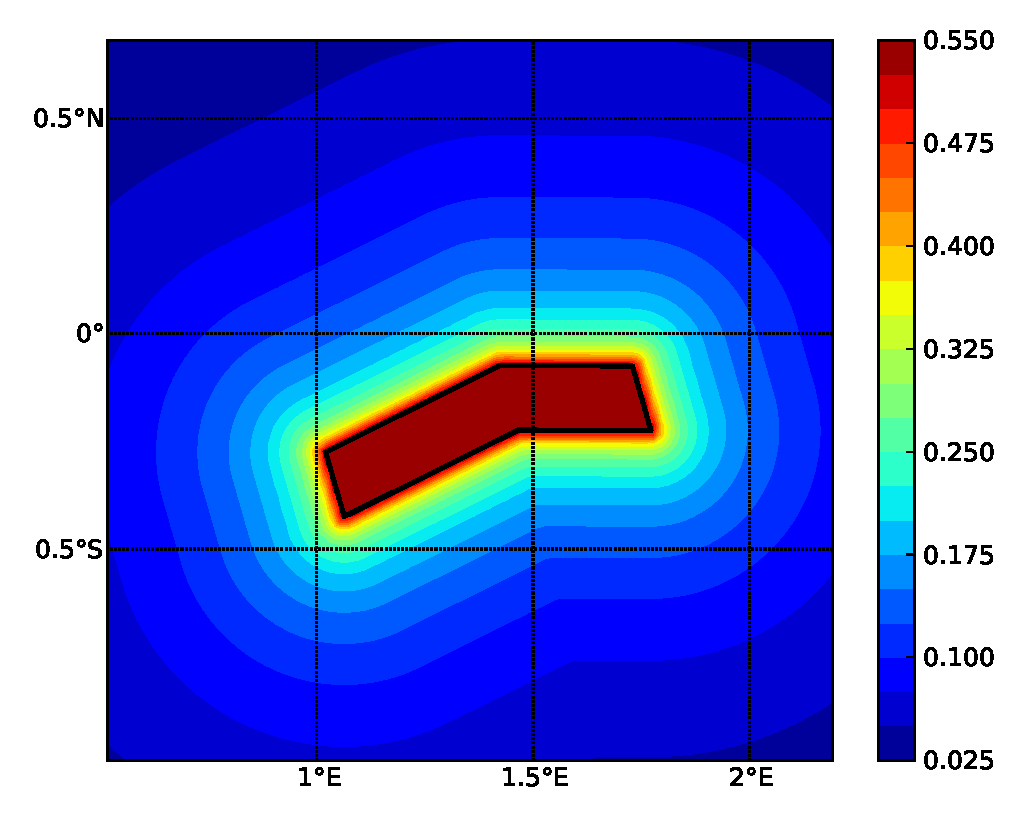
\includegraphics[width=7cm]{./figures/hazard/char_fault2.eps}} 
\subcaptionbox{}
{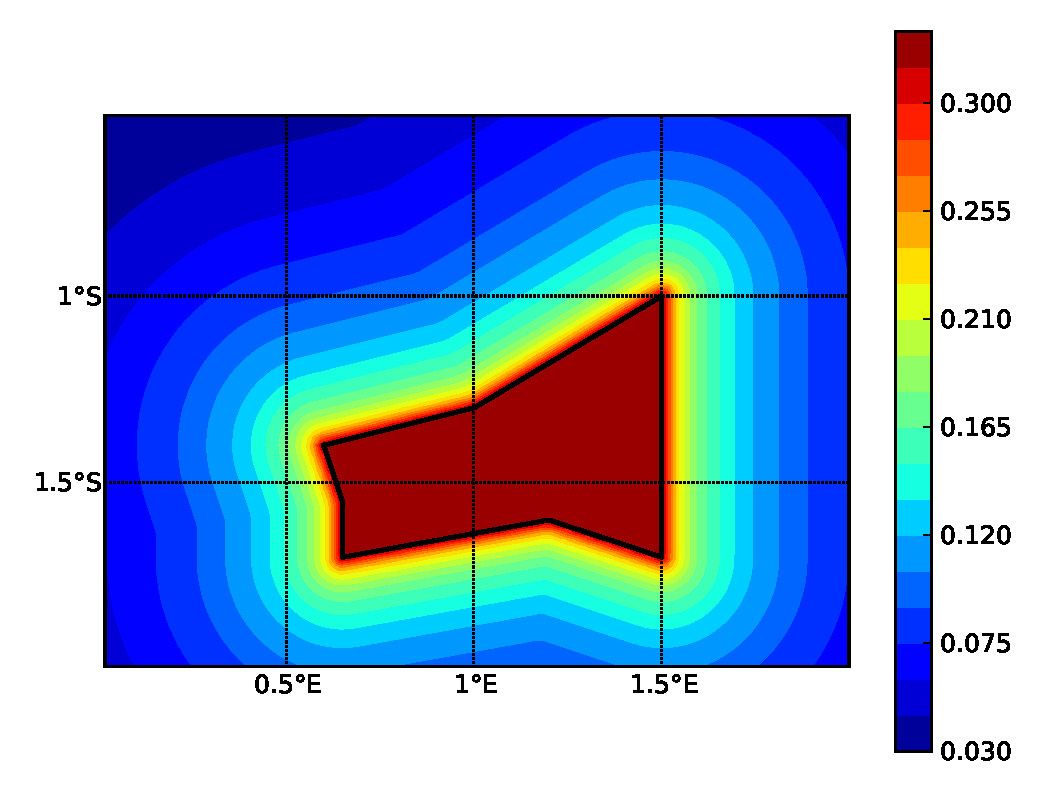
\includegraphics[width=7cm]{./figures/hazard/char_fault3.eps}} 
\subcaptionbox{}
{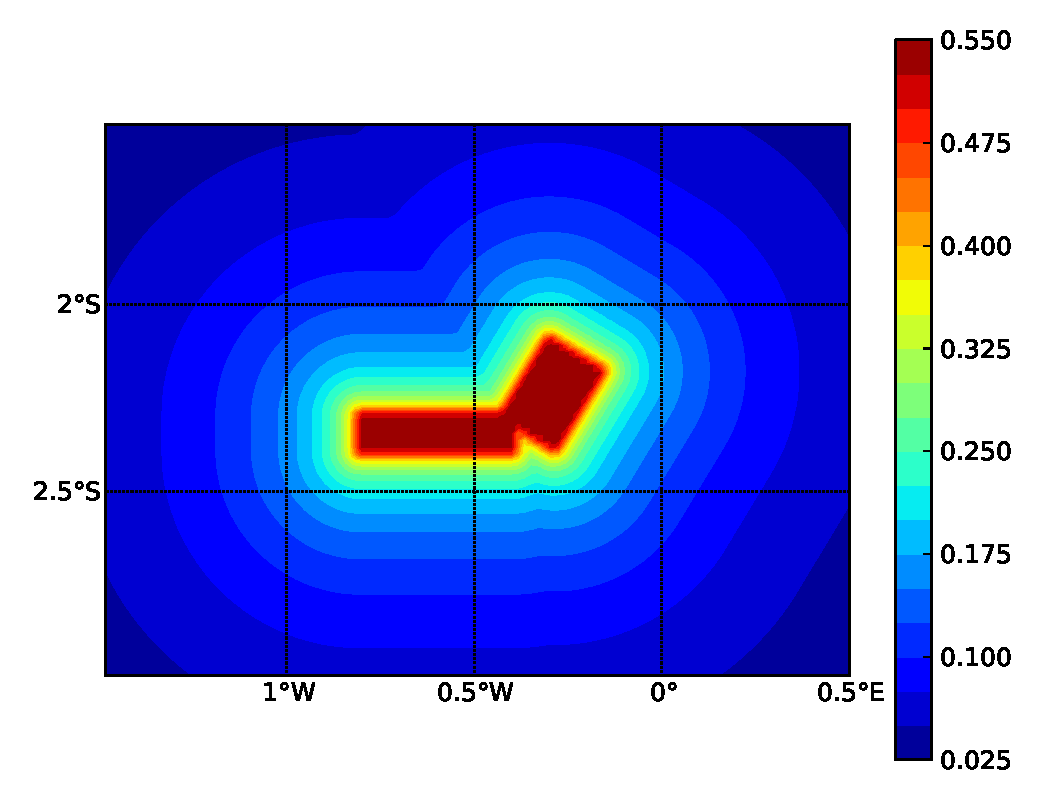
\includegraphics[width=7cm]{./figures/hazard/char_fault1.eps}} 
\caption{Hazard maps (for PGA, 10\% in 50 years) as obtained from 
    characteristic fault sources with simple fault
    geometry (e), complex fault geometry (f), and collection of 
    planar surfaces (g)}
\label{fig:hazard_maps2}
\end{figure}

\clearpage
\subsubsection{Classical PSHA with non trivial logic trees}
Three demos are provided to illustrate how the logic tree formalism can 
be used to express epistemic uncertainties in seismic hazard analysis.\\

LogicTreeCase1ClassicalPSHA shows an example of logic tree defining two 
alternative source models, with sources belonging to two different
tectonic region types, and with two alternative GMPEs for each tectonic 
region type.
The source model logic tree is therefore defined in the following way:
\begin{Verbatim}[frame=single, commandchars=\\\{\}, fontsize=\normalsize]
<?xml version="1.0" encoding="UTF-8"?>
<nrml xmlns:gml="http://www.opengis.net/gml"
      xmlns="http://openquake.org/xmlns/nrml/0.4">
    <logicTree logicTreeID="lt1">

        <logicTreeBranchingLevel branchingLevelID="bl1">

            <logicTreeBranchSet uncertaintyType="sourceModel"
                                branchSetID="bs1">
                <logicTreeBranch branchID="b1">
                    <uncertaintyModel>
                      source_model_1.xml
                    </uncertaintyModel>
                    <uncertaintyWeight>0.5</uncertaintyWeight>
                </logicTreeBranch>
                <logicTreeBranch branchID="b2">
                    <uncertaintyModel>
                       source_model_2.xml
                    </uncertaintyModel>
                    <uncertaintyWeight>0.5</uncertaintyWeight>
                </logicTreeBranch>
            </logicTreeBranchSet>

        </logicTreeBranchingLevel>

    </logicTree>
</nrml>
\end{Verbatim}
The two source models are defined in two separate files 
\texttt{source\_\-model\_\-1.xml} and \texttt{source\_\-model\_\-2.xml} each
one associated to a corresponding weight (0.5 for both).\\
The GSIM logic tree file contains the following structure:
\begin{Verbatim}[frame=single, commandchars=\\\{\}, fontsize=\normalsize]
<?xml version="1.0" encoding="UTF-8"?>

<nrml xmlns:gml="http://www.opengis.net/gml"
      xmlns="http://openquake.org/xmlns/nrml/0.4">
    <logicTree logicTreeID='lt1'>

        <logicTreeBranchingLevel branchingLevelID="bl1">
            <logicTreeBranchSet uncertaintyType="gmpeModel"
               applyToTectonicRegionType="Active Shallow Crust"
               branchSetID="bs1">
                <logicTreeBranch branchID="b11">
                   <uncertaintyModel>
                      BooreAtkinson2008
                   </uncertaintyModel>
                   <uncertaintyWeight>0.5</uncertaintyWeight>
                </logicTreeBranch>
                <logicTreeBranch branchID="b12">
                   <uncertaintyModel>
                      ChiouYoungs2008
                   </uncertaintyModel>
                   <uncertaintyWeight>0.5</uncertaintyWeight>
                </logicTreeBranch>
            </logicTreeBranchSet>
        </logicTreeBranchingLevel>

        <logicTreeBranchingLevel branchingLevelID="bl2">
            <logicTreeBranchSet uncertaintyType="gmpeModel"
              applyToTectonicRegionType="Stable Continental Crust"
              branchSetID="bs2">
              <logicTreeBranch branchID="b21">
                <uncertaintyModel>
                   ToroEtAl2002</uncertaintyModel>
                <uncertaintyWeight>0.5</uncertaintyWeight>
                </logicTreeBranch>
                <logicTreeBranch branchID="b22">
                  <uncertaintyModel>
                     Campbell2003</uncertaintyModel>
                  <uncertaintyWeight>0.5</uncertaintyWeight>
                </logicTreeBranch>
            </logicTreeBranchSet>
        </logicTreeBranchingLevel>

    </logicTree>
</nrml>
\end{Verbatim}
The source model contains sources belonging to Active Shallow Crust and 
Stable Continental Crust, therefore the
GSIM logic tree defines two branching levels, one for each considered 
tectonic region type. Moreover for each tectonic
region a branch set with two GMPEs is defined: Boore and Atkinson 
2008 and Chiou and Youngs 2008 for Active
Shallow Crust and Toro et al. 2003 and Campbell 2003 for Stable Continental 
Crust. By processing the above logic tree
files using the logic tree path enumeration mode (enabled by setting in the 
configuration file \texttt{number\_\-of\_\-logic\_\-tree\_\-samples = 0})
hazard results are computed for 8 logic tree paths (2 source models x 2 GMPEs
for Active x 2 GMPEs for Stable).\\

LogicTreeCase2ClassicalPSHA defines a single source model consisting of 
only two sources (area and simple fault) belonging to different
tectonic region types (Active Shallow Crust and Stable Continental Region) 
and both characterized by a truncated Gutenberg-Richter distribution.
The logic tree defines uncertainties for G-R a and b values (three possible
pairs for each source), maximum magnitude (three values for each source) 
and uncertainties on the GMPEs for each tectonic region type (two GMPE per 
region type).\\
To accommodate such a structure the GSIM logic tree is defined in the
following way:
\begin{Verbatim}[frame=single, commandchars=\\\{\}, fontsize=\normalsize]
<?xml version="1.0" encoding="UTF-8"?>
<nrml xmlns:gml="http://www.opengis.net/gml"
      xmlns="http://openquake.org/xmlns/nrml/0.4">
    <logicTree logicTreeID="lt1">

        <logicTreeBranchingLevel branchingLevelID="bl1">
            <logicTreeBranchSet uncertaintyType="sourceModel"
                                branchSetID="bs1">
                <logicTreeBranch branchID="b11">
                    <uncertaintyModel>
                     source_model.xml
                    </uncertaintyModel>
                    <uncertaintyWeight>1.0</uncertaintyWeight>
                </logicTreeBranch>
            </logicTreeBranchSet>
        </logicTreeBranchingLevel>

        <logicTreeBranchingLevel branchingLevelID="bl2">
            <logicTreeBranchSet uncertaintyType="abGRAbsolute"
                                applyToSources="1"
                                branchSetID="bs21">
                <logicTreeBranch branchID="b21">
                    <uncertaintyModel>4.6 1.1</uncertaintyModel>
                    <uncertaintyWeight>0.333</uncertaintyWeight>
                </logicTreeBranch>
                <logicTreeBranch branchID="b22">
                    <uncertaintyModel>4.5 1.0</uncertaintyModel>
                    <uncertaintyWeight>0.333</uncertaintyWeight>
                </logicTreeBranch>
                <logicTreeBranch branchID="b23">
                    <uncertaintyModel>4.4 0.9</uncertaintyModel>
                    <uncertaintyWeight>0.334</uncertaintyWeight>
                </logicTreeBranch>
            </logicTreeBranchSet>
        </logicTreeBranchingLevel>

        <logicTreeBranchingLevel branchingLevelID="bl3">
            <logicTreeBranchSet uncertaintyType="abGRAbsolute"
                                applyToSources="2"
                                branchSetID="bs31">
                <logicTreeBranch branchID="b31">
                    <uncertaintyModel>3.3 1.0</uncertaintyModel>
                    <uncertaintyWeight>0.333</uncertaintyWeight>
                </logicTreeBranch>
                <logicTreeBranch branchID="b32">
                    <uncertaintyModel>3.2 0.9</uncertaintyModel>
                    <uncertaintyWeight>0.333</uncertaintyWeight>
                </logicTreeBranch>
                <logicTreeBranch branchID="b33">
                    <uncertaintyModel>3.1 0.8</uncertaintyModel>
                    <uncertaintyWeight>0.334</uncertaintyWeight>
                </logicTreeBranch>
            </logicTreeBranchSet>
        </logicTreeBranchingLevel>

        <logicTreeBranchingLevel branchingLevelID="bl4">
            <logicTreeBranchSet uncertaintyType="maxMagGRAbsolute"
                                applyToSources="1"
                                branchSetID="bs41">
                <logicTreeBranch branchID="b41">
                    <uncertaintyModel>7.0</uncertaintyModel>
                    <uncertaintyWeight>0.333</uncertaintyWeight>
                </logicTreeBranch>
                <logicTreeBranch branchID="b42">
                    <uncertaintyModel>7.3</uncertaintyModel>
                    <uncertaintyWeight>0.333</uncertaintyWeight>
                </logicTreeBranch>
                <logicTreeBranch branchID="b43">
                    <uncertaintyModel>7.6</uncertaintyModel>
                    <uncertaintyWeight>0.334</uncertaintyWeight>
                </logicTreeBranch>
            </logicTreeBranchSet>
        </logicTreeBranchingLevel>

        <logicTreeBranchingLevel branchingLevelID="bl5">
            <logicTreeBranchSet uncertaintyType="maxMagGRAbsolute"
                                applyToSources="2"
                                branchSetID="bs51">
                <logicTreeBranch branchID="b51">
                    <uncertaintyModel>7.5</uncertaintyModel>
                    <uncertaintyWeight>0.333</uncertaintyWeight>
                </logicTreeBranch>
                <logicTreeBranch branchID="b52">
                    <uncertaintyModel>7.8</uncertaintyModel>
                    <uncertaintyWeight>0.333</uncertaintyWeight>
                </logicTreeBranch>
                <logicTreeBranch branchID="b53">
                    <uncertaintyModel>8.0</uncertaintyModel>
                    <uncertaintyWeight>0.334</uncertaintyWeight>
                </logicTreeBranch>
            </logicTreeBranchSet>
        </logicTreeBranchingLevel>

    </logicTree>
</nrml>
\end{Verbatim}
The first branching level defines the source model. For each source, 
two branching levels are created, one defining
uncertainties on G-R a and b values (defined by setting 
\texttt{uncertaintyType="abGRAbsolute"}) and G-R maximum
magnitude (\texttt{uncertaintyType="maxMagGRAbsolute"}). 
%
It is important to notice that each branch set is applied
to a specific source by defining the attribute \texttt{apply\-To\-Sources}, 
followed by the source ID. The GSIM logic tree file is
the same as used for LogicTreeCase1ClassicalPSHA. By setting in the 
configuration file \texttt{number\_\-of\_\-logic\_\-tree\_\-samples = 0},
hazard results are obtained for 324 paths (1 source model x 3 (a, b) 
pairs for source 1 x  3 (a, b) pairs for source 2 x 3 max magnitude values
for source 1 x 3 max magnitude values for source 2 x 2 GMPEs for Active 
Shallow Crust X 2 GMPEs for Stable Continental Crust), see
figure \ref{fig:hazard_curves}.\\

\begin{figure} 
\centering 
\subcaptionbox{}
{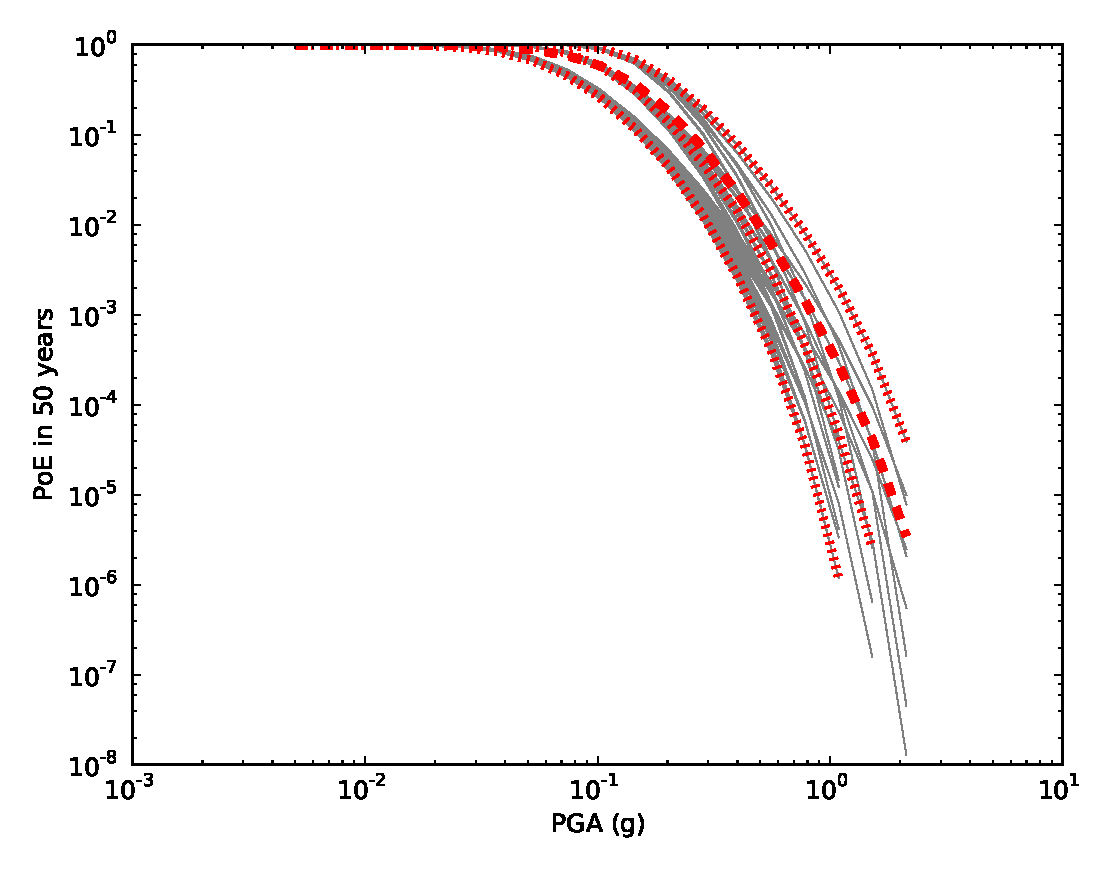
\includegraphics[width=9cm]{./figures/hazard/hazard-curves-ltcase2.eps}} 
\caption{Hazard curves as obtained from the LogicTreeCase2 demo. Solid gray 
    lines represent individual hazard curves from the different
    logic tree path (a total of 324 curves). The red dashed line represents the
    mean hazard curve, while the red dotted lines depict the quantile levels
    (0.15, 0.5, 0.95).}
\label{fig:hazard_curves}
\end{figure}

LogicTreeCase3ClassicalPSHA illustrates an example of logic tree defining 
relative uncertainties on G-R maximum magnitude and b value.
A single source model is considered containing two sources belonging to 
different tectonic region types and both characterized by a G-R 
magnitude frequency distribution. The source model logic tree is as follows:
\begin{Verbatim}[frame=single, commandchars=\\\{\}, fontsize=\normalsize]
<?xml version="1.0" encoding="UTF-8"?>
<nrml xmlns:gml="http://www.opengis.net/gml"
      xmlns="http://openquake.org/xmlns/nrml/0.4">
    <logicTree logicTreeID="lt1">

        <logicTreeBranchingLevel branchingLevelID="bl1">
            <logicTreeBranchSet uncertaintyType="sourceModel"
                                branchSetID="bs1">
                <logicTreeBranch branchID="b11">
                    <uncertaintyModel>
                     source_model.xml
                    </uncertaintyModel>
                    <uncertaintyWeight>1.0</uncertaintyWeight>
                </logicTreeBranch>
            </logicTreeBranchSet>
        </logicTreeBranchingLevel>

        <logicTreeBranchingLevel branchingLevelID="bl2">
            <logicTreeBranchSet uncertaintyType="bGRRelative"
                                branchSetID="bs21">
                <logicTreeBranch branchID="b21">
                    <uncertaintyModel>+0.1</uncertaintyModel>
                    <uncertaintyWeight>0.333</uncertaintyWeight>
                </logicTreeBranch>
                <logicTreeBranch branchID="b22">
                    <uncertaintyModel>0.0</uncertaintyModel>
                    <uncertaintyWeight>0.333</uncertaintyWeight>
                </logicTreeBranch>
                <logicTreeBranch branchID="b23">
                    <uncertaintyModel>-0.1</uncertaintyModel>
                    <uncertaintyWeight>0.334</uncertaintyWeight>
                </logicTreeBranch>
            </logicTreeBranchSet>
        </logicTreeBranchingLevel>

        <logicTreeBranchingLevel branchingLevelID="bl3">
            <logicTreeBranchSet uncertaintyType="maxMagGRRelative"
                                branchSetID="bs31">
                <logicTreeBranch branchID="b31">
                    <uncertaintyModel>0.0</uncertaintyModel>
                    <uncertaintyWeight>0.333</uncertaintyWeight>
                </logicTreeBranch>
                <logicTreeBranch branchID="b32">
                    <uncertaintyModel>+0.5</uncertaintyModel>
                    <uncertaintyWeight>0.333</uncertaintyWeight>
                </logicTreeBranch>
                <logicTreeBranch branchID="b33">
                    <uncertaintyModel>+1.0</uncertaintyModel>
                    <uncertaintyWeight>0.334</uncertaintyWeight>
                </logicTreeBranch>
            </logicTreeBranchSet>
        </logicTreeBranchingLevel>

    </logicTree>
</nrml>
\end{Verbatim}
After the first branching level defining the source model, two 
additional branching levels are defined, one defining
relative uncertainties on b value (\texttt{bGR\-Rel\-a\-tive} applied 
consistently to all sources in the source model)
and the second uncertainties on maximum magnitude (\texttt{maxMagGRRelative}). 
Similarly to the other cases, two GMPEs are considered for each tectonic 
region type and therefore the total number of logic tree path is 36
(1 source model x 3 b value increments x 3 maximum magnitude increments 
x 2 GMPE for Active x 2 GMPEs for Stable)

\subsubsection{Event Based PSHA}
A demo showing an example of Event Based calculation is provided with the 
following configuration file:
\begin{Verbatim}[frame=single, commandchars=\\\{\}, fontsize=\normalsize]
[general]

description = Event Based PSHA using Area Source
calculation_mode = event_based
random_seed = 23

[geometry]

sites = 0.5 -0.5

[logic_tree]

number_of_logic_tree_samples = 0

[erf]

rupture_mesh_spacing = 2
width_of_mfd_bin = 0.1
area_source_discretization = 5.0

[site_params]

reference_vs30_type = measured
reference_vs30_value = 600.0
reference_depth_to_2pt5km_per_sec = 5.0
reference_depth_to_1pt0km_per_sec = 100.0

[calculation]

source_model_logic_tree_file = source_model_logic_tree.xml
gsim_logic_tree_file = gmpe_logic_tree.xml
investigation_time = 50.0
intensity_measure_types = PGA
intensity_measure_types_and_levels = {"PGA": [...]}
truncation_level = 3
maximum_distance = 200.0

[event_based_params]

ses_per_logic_tree_path = 100
ground_motion_correlation_model =
ground_motion_correlation_params =

[output]

export_dir = ...
ground_motion_fields = true
hazard_curves_from_gmfs = true
mean_hazard_curves = false
quantile_hazard_curves =
hazard_maps = true
poes = 0.1
\end{Verbatim}
The source model consist of one source (area). 100 stochastic event sets 
are generated (\texttt{ses\_\-per\_\-logic\_\-tree\_\-path = 100}) (an 
example can be seen in figure \ref{fig:ses}). Ground motion fields are 
computed (\texttt{ground\_\-motion\_\-fields = true}, figure \ref{fig:gmfs}) 
and also hazard curves from ground motion fields are
extracted (\texttt{hazard\_\-curves\_\-from\_\-gmfs = true}).
The corresponding hazard maps for 0.1 probability are also calculated
(\texttt{hazard\_\-maps = true})

\begin{figure} 
\centering 
\subcaptionbox{}
{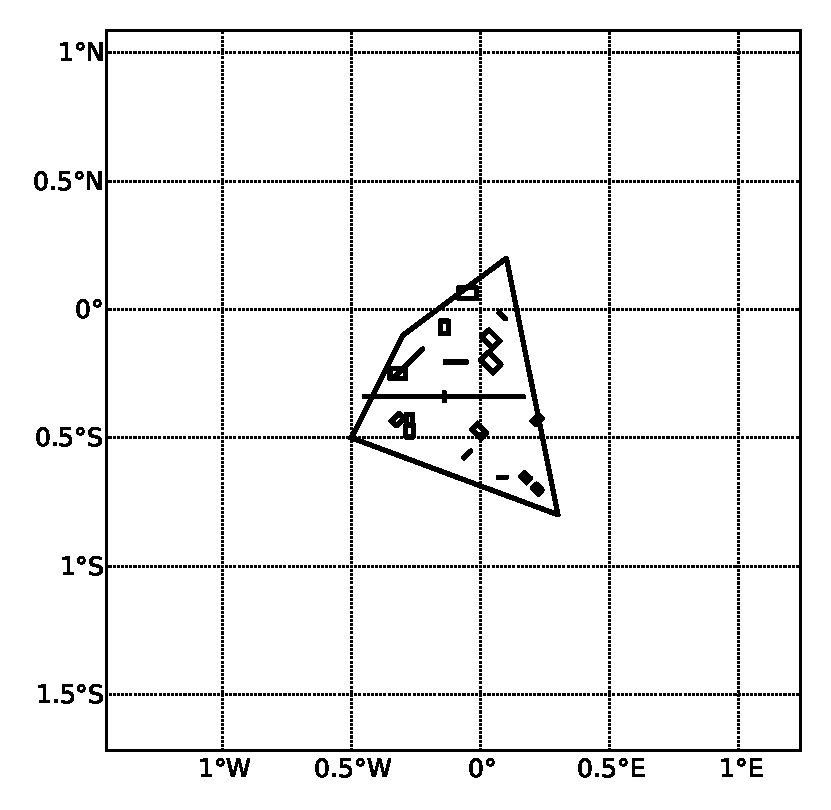
\includegraphics[width=9cm]{./figures/hazard/ses.eps}} 
\caption{A stochastic event set generated with the event based PSHA demo. 
    The area source defines a nodal plane distribution which distributes 
    events among vertical and dipping (50 degrees) faults with equal weights. 
    Vertical ruptures are then distributed equally in the range 0-180 degrees 
    while the dipping ones in the range 0-360, both with a step of 45 degrees.}
\label{fig:ses}
\end{figure}

\begin{figure} 
\centering 
\subcaptionbox{}
{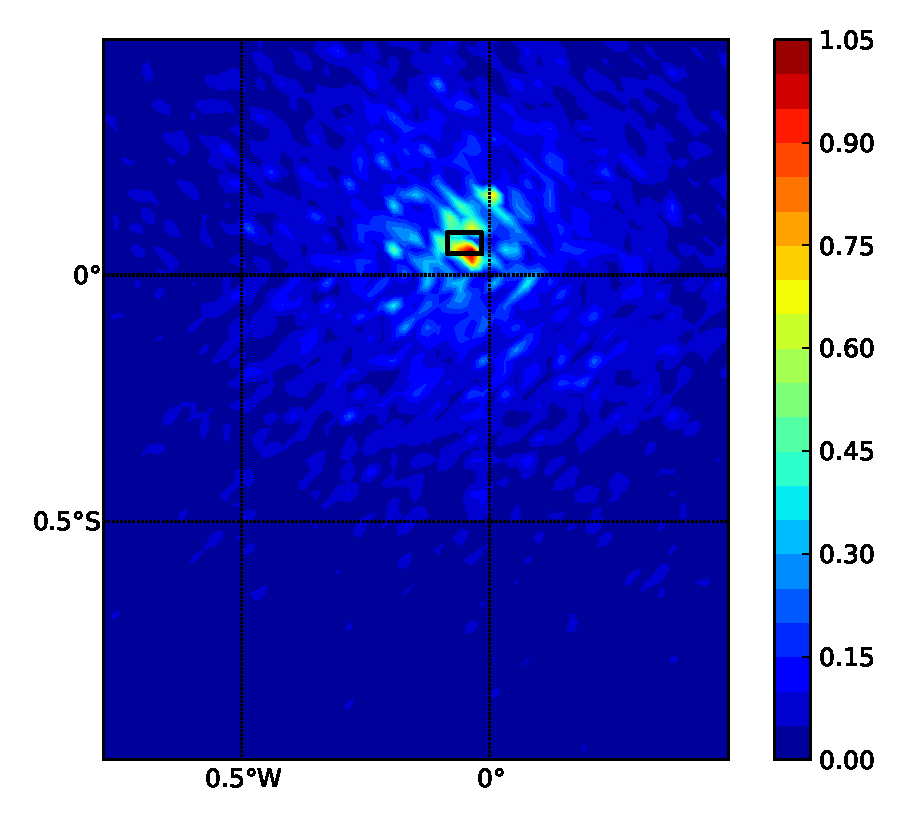
\includegraphics[width=6cm]{./figures/hazard/gmf-no-corr.eps}} 
\subcaptionbox{}
{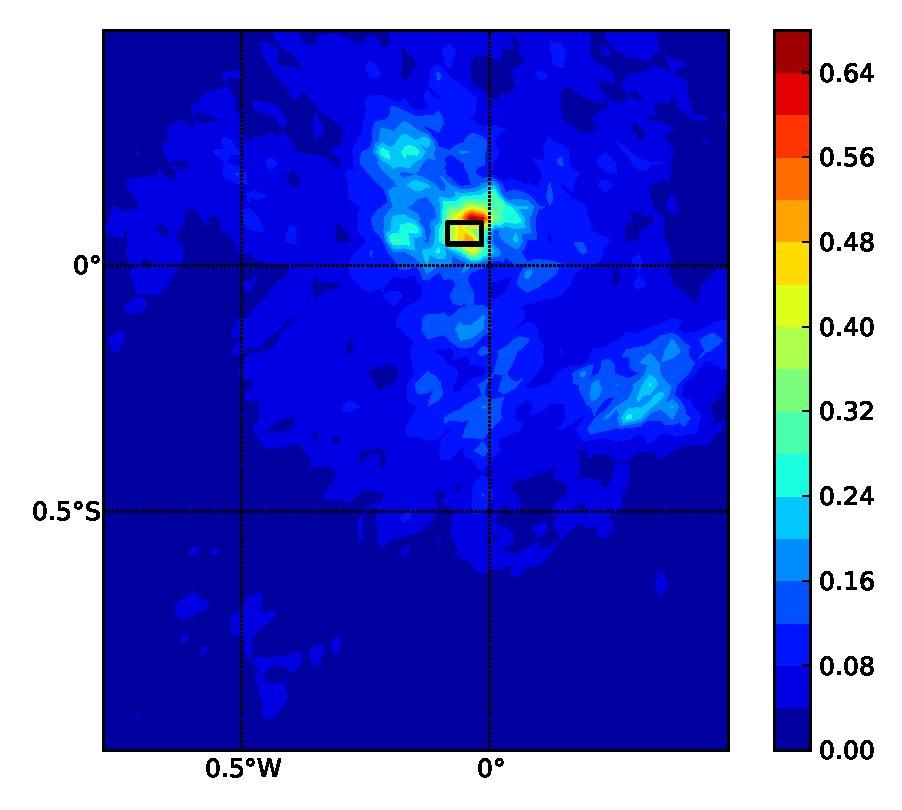
\includegraphics[width=6cm]{./figures/hazard/gmf-corr.eps}} 
\caption{Ground motion fields (PGA) with no spatial correlations (a) and with spatial correlation (b)}
\label{fig:gmfs}
\end{figure}

\subsubsection{Disaggregation}
An example of disaggregation calculation is given considering a source model 
consisting of two sources (area and simple fault) belonging to two different 
tectonic region types.

The calculation is defined with the following configuration file:
\begin{Verbatim}[frame=single, commandchars=\\\{\}, fontsize=\normalsize]
[general]

description = ...
calculation_mode = disaggregation
random_seed = 23

[geometry]

sites = 0.5 -0.5

[logic_tree]

number_of_logic_tree_samples = 0

[erf]

rupture_mesh_spacing = 2
width_of_mfd_bin = 0.1
area_source_discretization = 5.0

[site_params]

reference_vs30_type = measured
reference_vs30_value = 600.0
reference_depth_to_2pt5km_per_sec = 5.0
reference_depth_to_1pt0km_per_sec = 100.0

[calculation]

source_model_logic_tree_file = source_model_logic_tree.xml
gsim_logic_tree_file = gmpe_logic_tree.xml
investigation_time = 50.0
intensity_measure_types_and_levels = {"PGA": [...]}
truncation_level = 3
maximum_distance = 200.0

[disaggregation]

poes_disagg = 0.1
mag_bin_width = 1.0
distance_bin_width = 10.0
coordinate_bin_width = 0.2
num_epsilon_bins = 3

[output]

export_dir = ...
\end{Verbatim}
Disaggregation matrices are computed for a single site (located between the two sources) for a ground motion value corresponding to a probability value equal to 0.1
(\texttt{poes\_\-disagg = 0.1}). Magnitude values are classified in one magnitude unit bins (\texttt{mag\_\-bin\_\-width = 1.0}), distances in bins of 10 km
(\texttt{distance\_\-bin\_\-width = 10.0}), coordinates in bins of 0.2 degrees (\texttt{coordinate\_\-bin\_\-width = 0.2}). 3 epsilons bins are considered (\texttt{num\_\-epsilon\_\-bins = 3}).

\begin{comment}
The demo allows to compute 

\section{Demo 01 - Classical PSHA}

% -----------------------------------------------------------------------------
\section{Demo 02 - Classical PSHA: simple logic tree}
This demo contains simple logic tree structures accounting for epistemic
uncertainties in the seismic source and ground motion intensity models.

The seismic source model incorporates epistemic uncertainty about the 
value of the maximum magnitude of the magnitude-frequency distribution 
used.
%
The ground motion intensity model includes uncertainty about the ground
motion prediction equations to be used in the calculation of hazard.

Given that the overall structure of the logic tree is not particularly
complex and assuming that uncertainties are fully correlated we decide 
to compute all the possible realisations of the logic tree by fixing 
the \texttt{number\_\-of\_\-logic\_\-tree\_\-samples} parameter in the 
configuration file to zero.
\begin{Verbatim}[frame=single, commandchars=\\\{\}, fontsize=\normalsize]
[logic_tree]
number_of_logic_tree_samples = 0
\end{Verbatim}

Let's now run the OpenQuake:
\begin{Verbatim}[frame=single, fontsize=\normalsize]
user@ubuntu:~/demos/classical_psha_simple_lt$ openquake \ 
--rh job_1strike.ini 
\end{Verbatim}

This is the list of results that we get at the end of this calculation:
\begin{Verbatim}[frame=single, commandchars=\\\{\}, fontsize=\normalsize]
Calculation 8 results:
id | output_type | name
5 | hazard_curve | hc-rlz-10
6 | hazard_curve | hc-rlz-7
7 | hazard_curve | hc-rlz-8
8 | hazard_curve | hc-rlz-9
9 | hazard_curve | hc-rlz-11
10 | hazard_curve | hc-rlz-12
11 | hazard_map | hazard-map(0.1)-PGA-rlz-10
12 | hazard_map | hazard-map(0.1)-PGA-rlz-7
13 | hazard_map | hazard-map(0.1)-PGA-rlz-8
14 | hazard_map | hazard-map(0.1)-PGA-rlz-9
15 | hazard_map | hazard-map(0.1)-PGA-rlz-11
16 | hazard_map | hazard-map(0.1)-PGA-rlz-12
\end{Verbatim}
OpenQuake produced six hazard curves and six hazard maps i.e. one
result for each leaf of the logic tree. 
\end{comment}

   \cleardoublepage

% ------------------------------------------------------ Part III: Risk Module -
\thispagestyle{empty}
\part{Risk}

\chapterimage{figures/chapter_head.pdf} % Chapter heading image
\chapter{Introduction to the Risk Module}
   \label{chap:riskintro}
	\index{OpenQuake-engine!Risk}

The seismic risk results are calculated using the \gls{acr:risklib}, 
an open-source suite of tools for seismic risk assessment and
loss estimation. This library is written in the Python programming language
and available in the form of a ``developers'' release at the following location:
\href{https://github.com/gem/oq-engine/tree/master/openquake/risklib}{https://github.com/gem/oq-engine/tree/master/openquake/risklib}.

The risk component of the \glsdesc{acr:oqe} can compute both scenario-based and
probabilistic seismic damage and risk using various approaches. The following
types of analysis are currently supported:

\begin{itemize}

    \item \textit{\textbf{Scenario Damage Assessment}}, for the
	calculation of damage distribution statistics for a portfolio of buildings
	from a single earthquake rupture scenario taking into account aleatory and
	epistemic ground-motion variability.

    \item \textit{\textbf{Scenario Risk Assessment}}, for the calculation of
	individual asset and portfolio loss statistics due to a single earthquake
	rupture scenario taking into account aleatory and epistemic ground-motion
	variability. Correlation in the vulnerability of different assets of the
	same typology can also be taken into consideration.

	\item \textit{\textbf{Classical Probabilistic Seismic Damage Analysis}}, for 
	the calculation of damage state probabilities over a specified time period,  
	and probabilistic collapse maps, starting from the hazard curves 
	computed following the classical integration procedure (\cite{cornell1968}, 
	\citet{mcguire1976}) as formulated by \cite{field2003}.

    \item \textit{\textbf{Classical Probabilistic Seismic Risk Analysis}}, for the
	calculation of loss curves and loss maps, starting from the hazard curves 
	computed following the classical integration procedure (\cite{cornell1968}, 
	\citet{mcguire1976}) as formulated by \cite{field2003}.

	\item \textit{\textbf{Stochastic Event Based Probabilistic Seismic Risk Analysis}}, 
	for the calculation of event loss tables starting from stochastic event sets.
	Other results such as loss-exceedance curves, probabilistic loss maps, 
	average annual losses, and insured loss statistics can be obtained by 
	post-processing the event loss tables.

    \item \textit{\textbf{Retrofit Benefit-Cost Ratio Analysis}}, which is
	useful in estimating the net-present value of the potential benefits of
	performing retrofitting for a portfolio of assets (in terms of decreased
	losses in seismic events), measured relative to the upfront cost of
	retrofitting.

\end{itemize}

Each calculation workflow has a modular structure, so that intermediate
results can be saved and analyzed. Moreover, each calculator can be
extended independently of the others so that additional calculation options
and methodologies can be easily introduced, without affecting the overall
calculation workflow. Each workflow is described in more detail in the
following sections.

\section{Scenario Damage Assessment}
\index{OpenQuake-engine!Risk calculation workflows!Scenario Damage Assessment}
\label{sec:workflow_scenario_damage}
The scenario damage calculator computes damage distribution statistics for all
assets in a given exposure model for a single specified earthquake rupture.
Damage distribution statistics include the mean and standard deviation of
damage fractions for different damage states. This calculator requires the
definition of a finite rupture model, an exposure model and a fragility model;
the main results are the damage distribution statistics per asset, aggregated
damage distribution statistics per taxonomy, aggregated damage distribution
statistics for the region, and collapse maps, which contain the spatial
distribution of the number or area of collapsed buildings throughout the
region of interest.

The rupture characteristics---i.e. the magnitude, hypocenter and fault
geometry---are modelled as deterministic in the scenario calculators. Multiple
realizations of different possible ground motion fields (GMFs) due to the
single rupture are generated, taking into consideration both the inter-event
variability of ground motions, and the intra-event residuals obtained from a
spatial correlation model for ground motion residuals. The use of logic trees
allows for the consideration of uncertainty in the choice of a ground motion
model for the given tectonic region.

As an alternative to computing the GMFs with OpenQuake, users can also provide
their own sets of GMFs as input to the scenario damage calculator.

For each GMF realization, damage fractions (the fraction of buildings in each
damage state) are estimated for every asset in the exposure model using the
provided fragility model, and finally the damage distribution statistics
(i.e., the mean damage fractions and standard deviation of damage fractions
for all damage states) across all realizations are calculated. The calculator
also provides aggregated damage distribution statistics for the portfolio,
such as mean damage fractions and standard deviation of damage fractions for
each taxonomy in the exposure model, and the mean damage fractions and
standard deviation of damage fractions for the entire region of study.

The required input files required for running a scenario damage calculation
and the resulting output files are depicted in Figure~\ref{fig:io-structure-scenario-damage}.

\begin{figure}[ht]
\centering
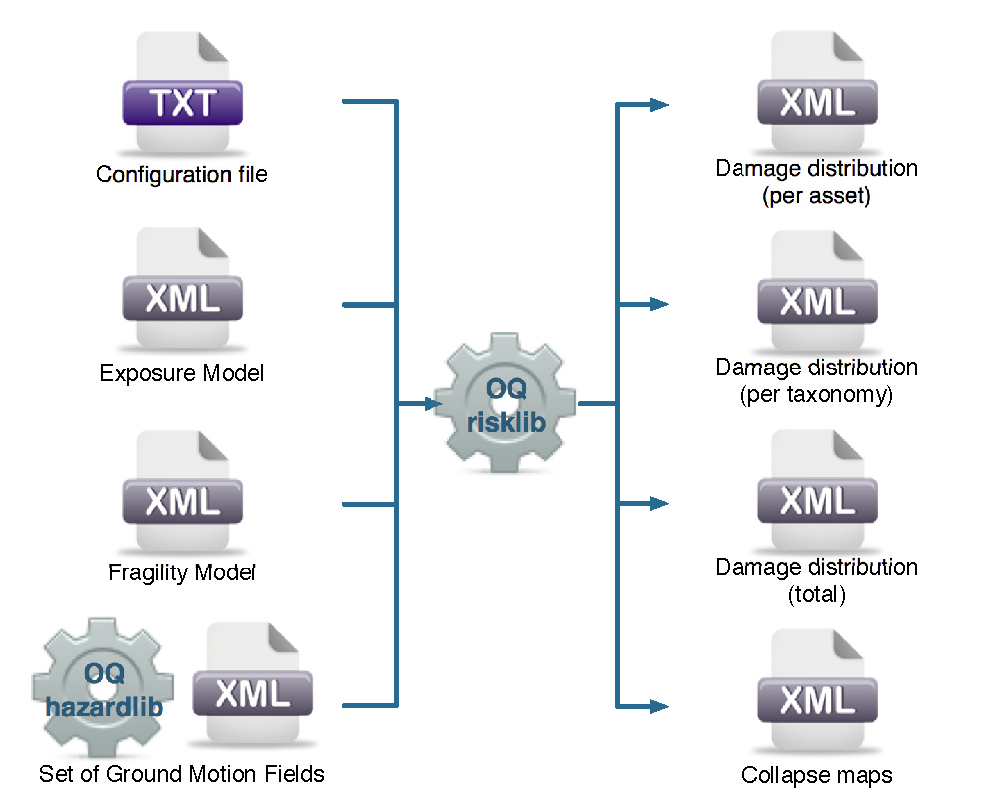
\includegraphics[width=9cm,height=7cm]{figures/risk/io-structure-scenario-damage.pdf}
\caption{Scenario Damage Calculator input/output structure.}
\label{fig:io-structure-scenario-damage}
\end{figure}

Starting with OpenQuake-engine v1.7, \gls{consequence model} files can also be
provided as inputs for a scenario damage calculation in addition to
\glspl{fragility model} files, in order to estimate consequences based on the
calculated damage distribution. The user may provide one \gls{consequence
model} file corresponding to each loss type (amongst structural,
nonstructural, contents, and business interruption) for which a fragility
model file is provided. Whereas providing a \gls{fragility model} file for at
least one loss type is mandatory for running a Scenario Damage calculation,
providing corresponding \gls{consequence model} files is optional.


\section{Scenario Risk Assessment}
\index{OpenQuake-engine!Risk calculation workflows!Scenario Risk Assessment}
\label{sec:workflow_scenario_risk}
The scenario risk calculator computes loss statistics for all \glspl{asset} in
a given \gls{exposuremodel} for a single specified earthquake rupture. Loss
statistics include the mean and standard deviation of ground-up losses and
insured losses for each loss type considered in the analysis. Loss statistics
can currently be computed for five different loss types using this calculator:
structural losses, nonstructural losses, contents losses, downtime losses, and
occupant fatalities. This calculator requires the definition of a finite
rupture model, an \gls{exposuremodel} and a \gls{vulnerabilitymodel} for each
loss type considered; the main results are the loss statistics per \gls{asset}
and mean loss maps.

The rupture characteristics---i.e. the magnitude, hypocenter and fault
geometry---are modelled as deterministic in the scenario calculators. Multiple
realizations of different possible ground motion fields (GMFs) due to the
single rupture are generated, taking into consideration both the inter-event
variability of ground motions, and the intra-event residuals obtained from a
spatial correlation model for ground motion residuals. The use of logic trees
allows for the consideration of uncertainty in the choice of a ground motion
model for the given tectonic region.

As an alternative to computing the GMFs with OpenQuake, users can also provide
their own sets of GMFs as input to the scenario risk calculator.

For each GMF realization, a loss ratio is sampled for every asset in the
\gls{exposuremodel} using the provided probabilistic \gls{vulnerabilitymodel}
taking into consideration the correlation model for vulnerability of different
assets of a given taxonomy. Finally loss statistics, i.e., the mean loss and
standard deviation of loss for both ground-up losses and insured losses across
all realizations, are calculated for each asset. Mean loss maps are also
generated by this calculator, describing the mean ground-up losses and mean
insured losses caused by the scenario event for the different assets in the
\gls{exposuremodel}.

The required input files required for running a scenario risk calculation and
the resulting output files are depicted in Figure~\ref{fig:io-structure-scenario-risk}.

\begin{figure}[ht]
\centering
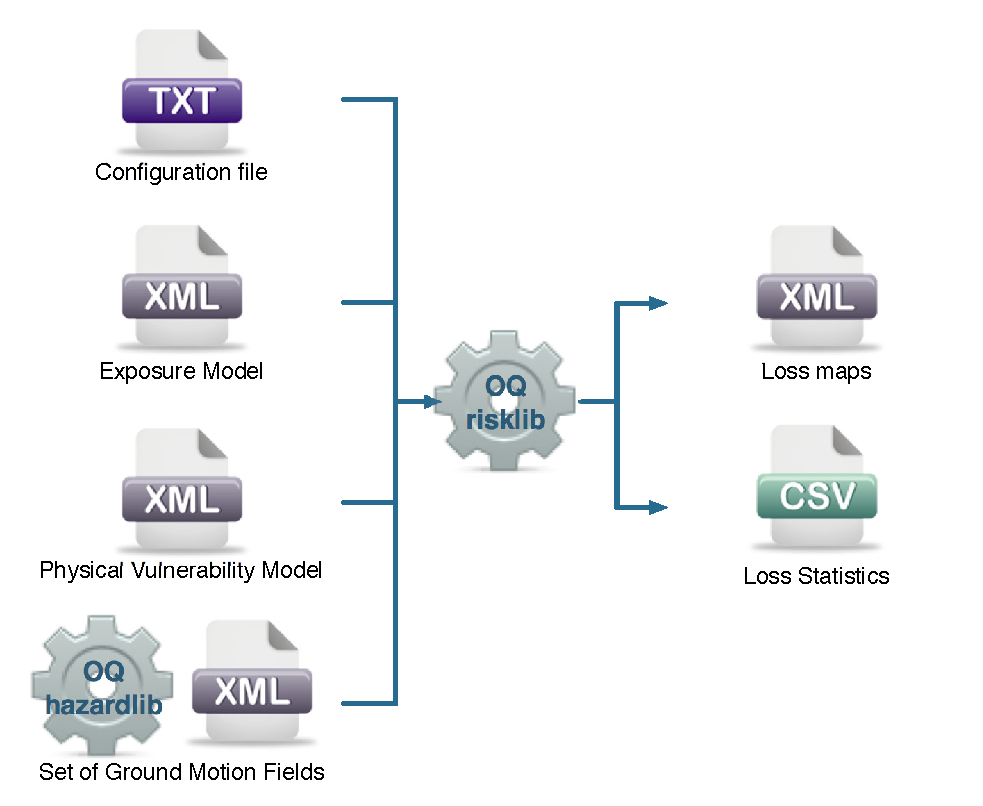
\includegraphics[width=9cm,height=7cm]{figures/risk/io-structure-scenario-risk.pdf}
\caption{Scenario Risk Calculator input/output structure.}
\label{fig:io-structure-scenario-risk}
\end{figure}

\section{Classical Probabilistic Seismic Damage Analysis}
\index{OpenQuake-engine!Risk calculation workflows!Classical Probabilistic Seismic Damage Analysis}
\label{sec:workflow_classical_damage}
The classical PSHA-based damage calculator integrates the fragility functions
for an asset with the seismic hazard curve at the location of the asset, to
give the expected damage distribution for the asset within a specified time
period. The calculator requires the definition of an exposure model, a
fragility model for each taxonomy represented in the exposure model, and
hazard curves calculated in the region of interest. The main results of this
calculator are the expected damage distribution for each asset, which describe
the probability of the asset being in different damage states, and collapse
maps for the region, which describe the probability of collapse for different
assets in the portfolio over the specified time period. Damage distribution
aggregated by taxonomy or of the total portfolio (considering all assets in
the exposure model) can not be extracted using this calculator, as the spatial
correlation of the ground motion residuals is not taken into consideration.

The hazard curves required for this calculator can be calculated by the
OpenQuake engine for all asset locations in the exposure model using the
classical PSHA approach \citep{cornell1968, mcguire1976}.

The required input files required for running a classical probabilistic damage
calculation and the resulting output files are depicted in Figure~\ref{fig:io-structure-classical-damage}.

\begin{figure}[ht]
\centering
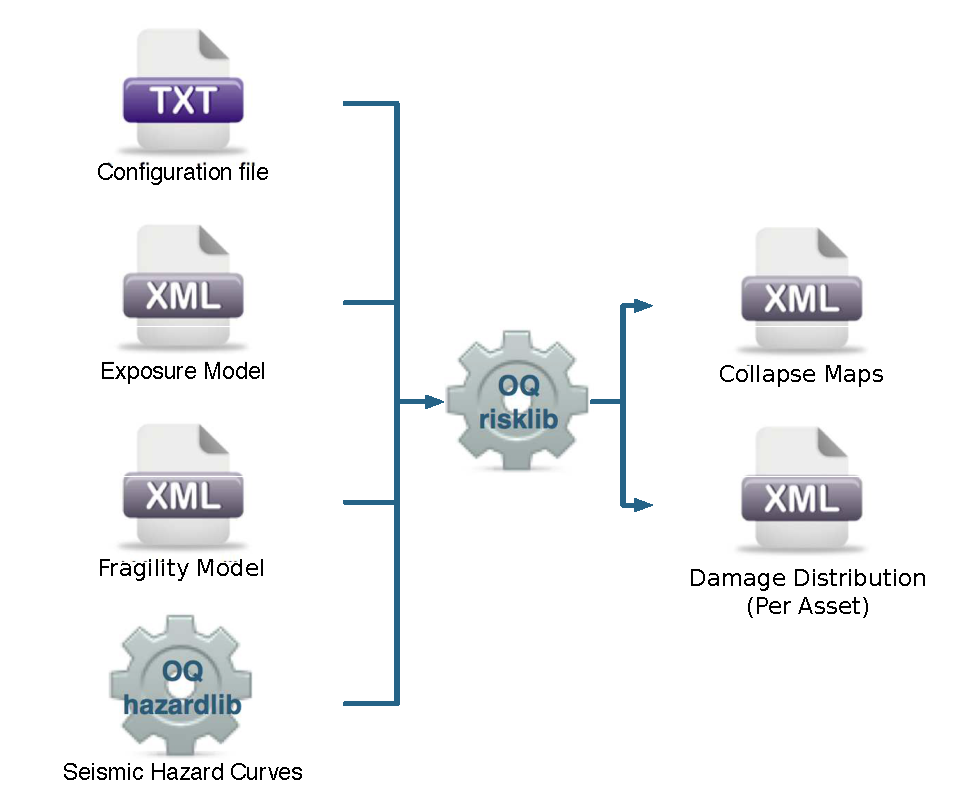
\includegraphics[width=9cm,height=7cm]{figures/risk/io-structure-classical-damage.pdf}
\caption{Classical PSHA-based Damage Calculator input/output structure.}
\label{fig:io-structure-classical-damage}
\end{figure}

\section{Classical Probabilistic Seismic Risk Analysis}
\index{OpenQuake-engine!Risk calculation workflows!Classical Probabilistic Seismic Risk Analysis}
\label{sec:workflow_classical_risk}
The classical PSHA-based risk calculator convolves through numerical
integration, the probabilistic vulnerability functions for an asset with the
seismic hazard curve at the location of the asset, to give the loss
distribution for the asset within a specified time period. The calculator
requires the definition of an exposure model, a vulnerability model for each
loss type of interest with vulnerability functions for each taxonomy
represented in the exposure model, and hazard curves calculated in the region
of interest. Loss curves and loss maps can currently be calculated for five
different loss types using this calculator: structural losses, nonstructural
losses, contents losses, downtime losses, and occupant fatalities. The main
results of this calculator are loss exceedance curves for each asset, which
describe the probability of exceedance of different loss levels over the
specified time period, and loss maps for the region, which describe the loss
values that have a given probability of exceedance over the specified time

Unlike the probabilistic event-based risk calculator, an aggregate loss curve
(considering all assets in the exposure model) can not be extracted using this
calculator, as the correlation of the ground motion residuals and
vulnerability uncertainty is not taken into consideration in this calculator.

The hazard curves required for this calculator can be calculated by the
OpenQuake engine for all asset locations in the exposure model using the
classical PSHA approach \citep{cornell1968, mcguire1976}. The use of logic-
trees allows for the consideration of model uncertainty in the choice of a
ground motion prediction equation for the different tectonic region types in
the region. Unlike what was described in the previous calculator, a total loss
curve (considering all assets in the exposure model) can not be extracted
using this calculator, as the correlation of the ground motion residuals and
vulnerability uncertainty is not taken into consideration.

The required input files required for running a classical probabilistic risk
calculation and the resulting output files are depicted in Figure~\ref{fig:io-structure-classical-risk}.

\begin{figure}[ht]
\centering
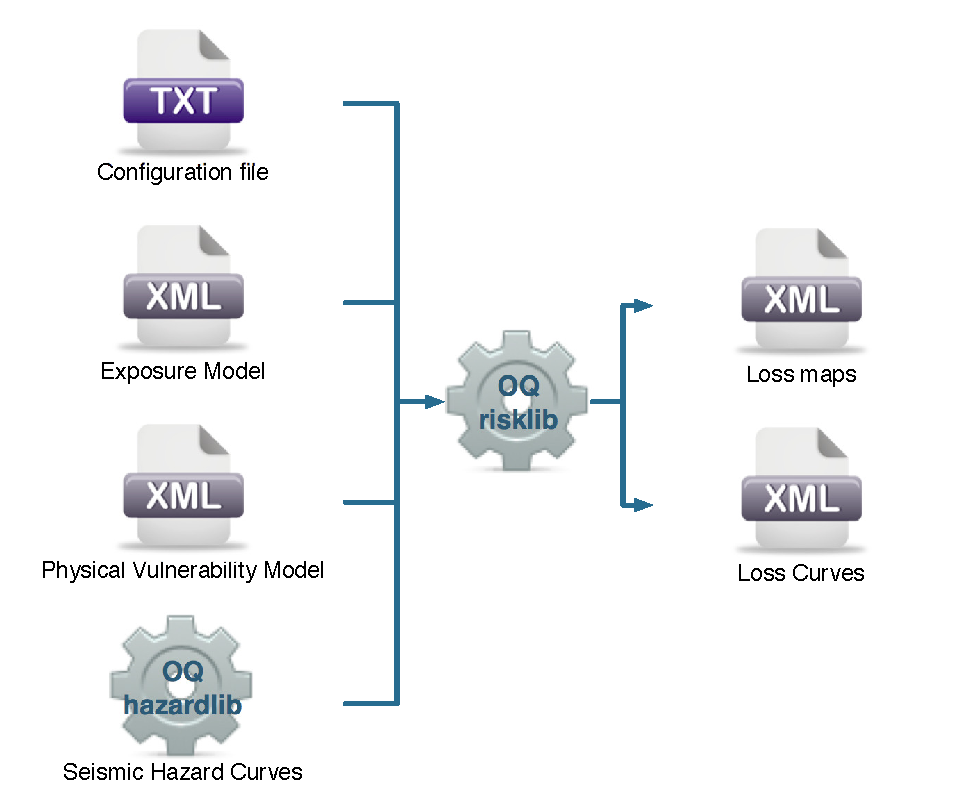
\includegraphics[width=9cm,height=7cm]{figures/risk/io-structure-classical-risk.pdf}
\caption{Classical PSHA-based Risk Calculator input/output structure.}
\label{fig:io-structure-classical-risk}
\end{figure}

\section{Stochastic Event Based Probabilistic Seismic Risk Analysis}
\index{OpenQuake-engine!Risk calculation workflows!Event-Based Probabilistic Seismic Risk Analysis}
\label{sec:workflow_event_based_risk}
This calculator employs an event-based Monte Carlo simulation approach to
probabilistic risk assessment in order to estimate the loss distribution for
individual assets and aggregated loss distribution for a spatially distributed
portfolio of assets within a specified time period. The calculator requires
the definition of an exposure model, a vulnerability model for each loss type
of interest with vulnerability functions for each taxonomy represented in the
exposure model, and a set of ground motion fields representative of the
seismicity of the region over the specified time period. Loss curves and loss
maps can currently be calculated for five different loss types using this
calculator: structural losses, nonstructural losses, contents losses, downtime
losses, and occupant fatalities. The main results of this calculator are loss
exceedance curves for each asset, which describe the probability of exceedance
of different loss levels over the specified time period, and loss maps for the
region, which describe the loss values that have a given probability of
exceedance over the specified time period. Aggregate loss exceedance curves
can be also be produced using this calculator; these describe the probability
of exceedance of different loss levels for all assets of a single taxonomy, or
for all assets in the portfolio, over the specified time period. Finally,
event loss tables can be produced using this calculator; these tables describe
the total loss across the portfolio for each seismic event in the stochastic
event set.

This calculator relies on the probabilistic event-based hazard calculator,
which simulates the seismicity of the chosen time period $T$ by producing a
\textit{stochastic event set} (also known as a \textit{synthetic catalog}).
For each rupture generated by a source, the number of occurrences in the given
time span $T$ is simulated by sampling the corresponding probability
distribution as given by $P_{rup}(k | T)$. A stochastic event set is therefore
a \textit{sample} of the full population of ruptures as defined by a seismic
source model. Each rupture is present zero, one or more times, depending on
its probability. Symbolically, we can define a stochastic event set ($SES$)
as:
\begin{align}
SES(T) = \left\{k \times rup,\;k\sim P_{rup}(k | T)\;\;\forall\;rup\;in\;Src\;\forall\;Src\;in\;SSM\right\}
\end{align}
where $k$, the number of occurrences, is a random sample of $P_{rup}(k | T)$,
and $k \times rup$ means that rupture $rup$ is repeated $k$ times in the
stochastic event set.

For each rupture or event in the stochastic event sets, a spatially correlated
ground motion field (GMF) realisation is generated, taking into consideration
both the inter-event variability of ground motions, and the intra-event
residuals obtained from a spatial correlation model for ground motion
residuals. The use of logic-trees allows for the consideration of uncertainty
in the choice of a seismic source model, in the choice of GMPE models for the
different tectonic regions, and in the choice of vulnerability functions for
the different taxonomy types in the exposure model.

For each GMF realization, a loss ratio is sampled for every asset in the
exposure model using the provided probabilistic vulnerability model, taking
into consideration the correlation model for vulnerability of different assets
of a given taxonomy. Finally loss exceedance curves are computed for both
ground-up losses and insured losses.

The required input files required for running a probabilistic stochastic
event-based risk calculation and the resulting output files are depicted in
Figure~\ref{fig:io-structure-event-based-risk}

\begin{figure}[ht]
\centering
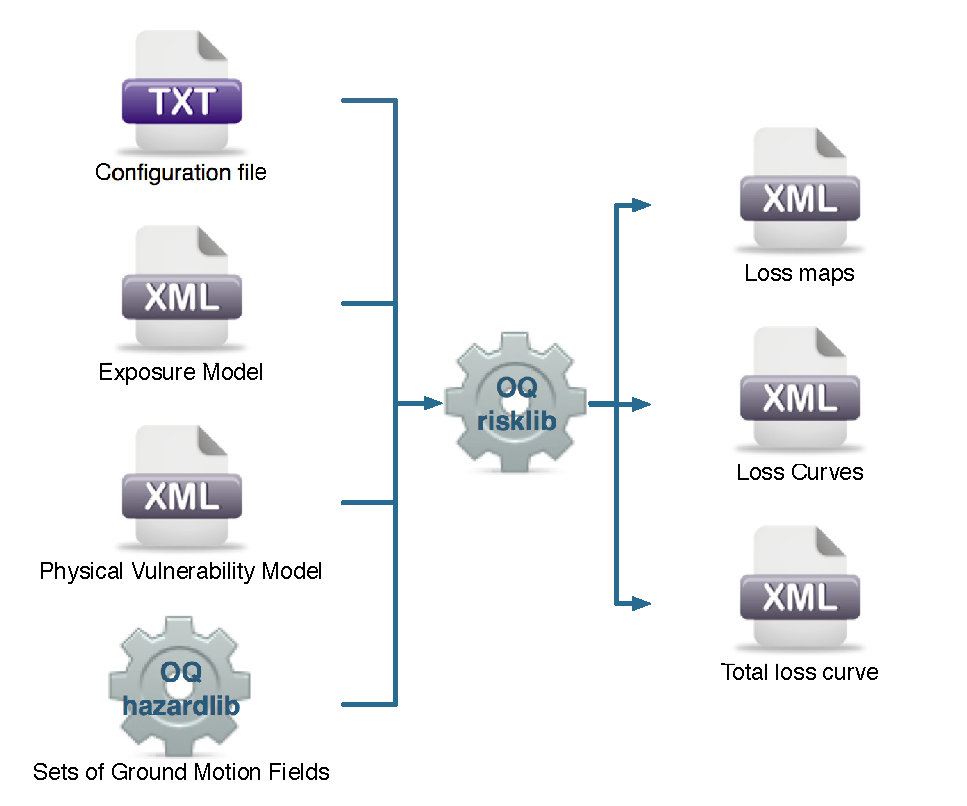
\includegraphics[width=9cm,height=7cm]{figures/risk/io-structure-event-based-risk.pdf}
\caption{Probabilistic Event-based Risk Calculator input/output structure.}
\label{fig:io-structure-event-based-risk}
\end{figure}

\section{Retrofit Benefit-Cost Ratio Analysis}
\index{OpenQuake-engine!Risk calculation workflows!Retrofit Benefit-Cost Ratio Analysis}
\label{sec:workflow_benefit_cost}
This calculator represents a decision-support tool for deciding whether the
employment of retrofitting measures to a collection of existing buildings is
advantageous from an economical point of view. For this assessment, the
expected losses considering the original and retrofitted configuration of the
buildings are estimated, and the economic benefit due to the better seismic
design is divided by the retrofitting cost, leading to the benefit/cost ratio.
These loss curves are computed using the previously described Classical PSHA-
based Risk calculator. The output of this calculator is a benefit/cost ratio
for each asset, in which a ratio above one indicates that employing a
retrofitting intervention is economically viable.

In Figure~\ref{fig:io-structure-benefit-cost}, the input/output structure for
this calculator is depicted.

\begin{figure}[ht]
\centering
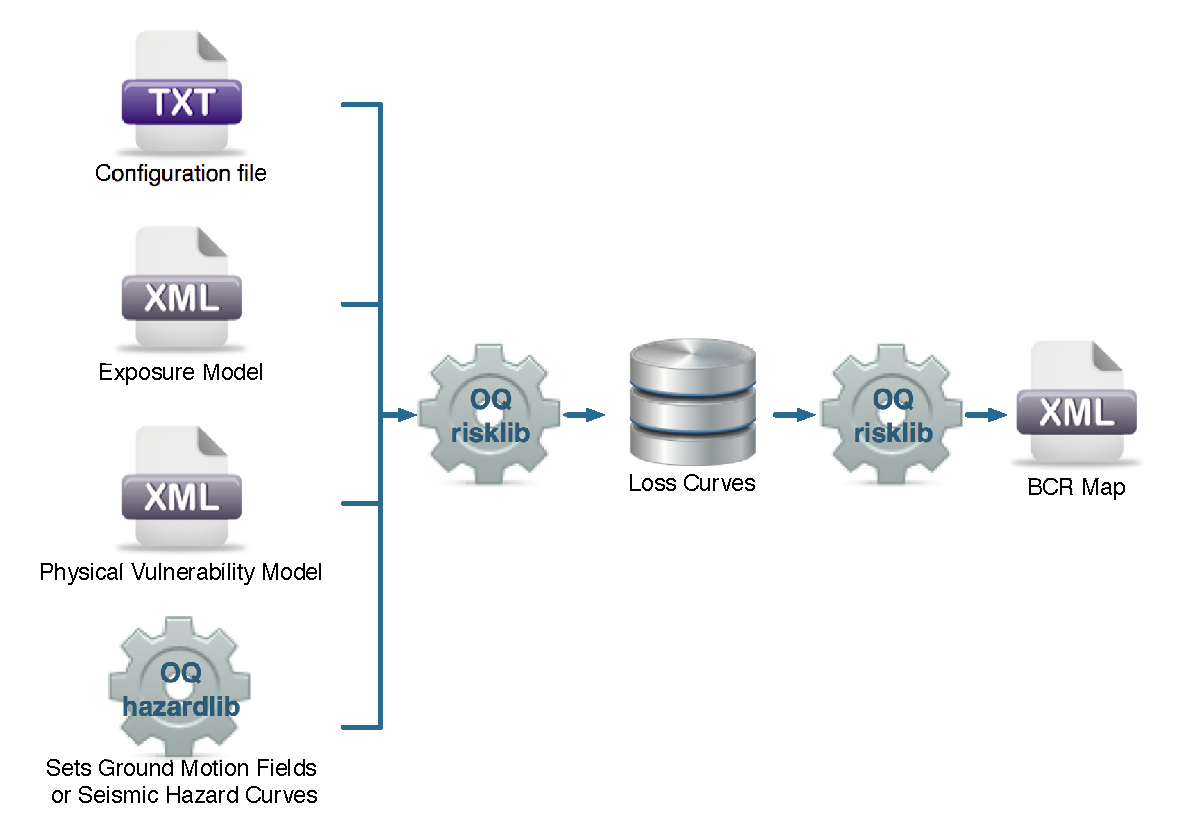
\includegraphics[width=10.5cm,height=7cm]{figures/risk/io-structure-benefit-cost.pdf}
\caption{Retrofitting Benefit/Cost Ratio Calculator input/output structure.}
\label{fig:io-structure-benefit-cost}
\end{figure}

For further information regarding the theoretical background of the
methodologies used for each calculator, users are referred to the OpenQuake-
engine Book (Risk).

\cleardoublepage
   \cleardoublepage

\chapterimage{figures/chapter_head.pdf} % Chapter heading image
\chapter{Risk Input Models}
   \label{chap:riskinputs}
   The following sections describe the basic inputs required for a risk
calculation, including exposure models, fragility models, consequence models,
and vulnerability models. In addition, each risk calculator also requires the
appropriate hazard inputs computed in the region of interest. Hazard inputs
include hazard curves for the classical probabilistic damage and risk
calculators, ground motion fields for the scenario damage and risk
calculators, or stochastic event sets for the probabilistic event based
calculators.


\section{Exposure Models}
\label{sec:exposure}
\emph{All} risk calculators in the OpenQuake-engine require an \gls{exposure
model} that needs to be provided in the NRML format. The information included
in an exposure model comprises a metadata section listing general information
about the exposure, followed by a cost conversions section that describes how
the different areas, costs, and occupancies for the assets will be specified,
followed by data regarding each individual asset in the portfolio.

A minimal exposure model comprising a single asset is shown in Listing~\ref{lst:input_exposure_minimal}.

\begin{listing}[htbp]
  \inputminted[firstline=1,firstnumber=1,fontsize=\footnotesize,frame=single,linenos,bgcolor=lightgray]{xml}{oqum/risk/Verbatim/input_exposure_minimal.xml}
  \caption{Example exposure model comprising a single asset}
  \label{lst:input_exposure_minimal}
\end{listing}

Let us take a look at each of the sections in the above example file in turn.
The first part of the file contains the metadata section:

\inputminted[firstline=5,firstnumber=5,lastline=8,fontsize=\footnotesize,frame=single,linenos,bgcolor=lightgray]{xml}{oqum/risk/Verbatim/input_exposure_minimal.xml}

The information in the metadata section is common to all of the assets in the
portfolio and needs to be incorporated at the beginning of every exposure
model file. There are a number of parameters that compose the metadata
section, which is intended to provide general information regarding the
\glspl{asset} within the \gls{exposure model}. These parameters are described
below:

\begin{itemize}

  \item \Verb+id+: a unique key used to identify the \gls{exposure model}

  \item \Verb+category+: an optional string used to define the type of
    \glspl{asset} being stored (e.g: buildings, lifelines)

  \item \Verb+taxonomySource+: an optional attribute used to define the
    \gls{taxonomy} being used to classify the \glspl{asset}

  \item \Verb+description+: a brief string with further information about the
    \gls{exposure model}

\end{itemize}


Next, let us look at the part of the file describing the area and cost
conversions:

\inputminted[firstline=10,firstnumber=10,lastline=15,fontsize=\footnotesize,frame=single,linenos,bgcolor=lightgray]{xml}{oqum/risk/Verbatim/input_exposure_minimal.xml}

Notice that the \Verb+costType+ element defines a \Verb+name+, a \Verb+type+, 
and a \Verb+unit+ attribute.

The NRML schema for the exposure model allows the definition of a structural
cost, a nonstructural components cost, a contents cost, and a business
interruption or downtime cost for each asset in the portfolio. Thus, the valid
values for the \Verb+name+ attribute of the \Verb+costType+ element are the
following:

\begin{itemize}

  \item \Verb+structural+: used to specify the structural replacement cost
    of assets

  \item \Verb+nonstructural+: used to specify the replacement cost for the
    nonstructural components of assets

  \item \Verb+contents+: used to specify the contents replacement cost

  \item \Verb+business_interruption+: used to specify the cost that will be 
    incurred per unit time that a damaged asset remains closed following an 
    earthquake

\end{itemize}

The exposure model shown in the example above defines only the structural
values for the assets. However, multiple cost types can be defined for each
asset in the same exposure model.

The \Verb+unit+ attribute of the \Verb+costType+ element is used for
specifying the currency unit for the corresponding cost type. Note that the
OpenQuake-engine itself is agnostic to the currency units; the \Verb+unit+ is
thus a descriptive attribute which is used by OpenQuake-engine to annotate the
results of a risk assessment. This attribute can be set to any valid Unicode
string.

The \Verb+type+ attribute of the \Verb+costType+ element specifies whether the
costs will be provided as an aggregated value for an asset, or per building or
unit comprising an asset, or per unit area of an asset. The valid values for
the \Verb+type+ attribute of the \Verb+costType+ element are the following:

\begin{itemize}

  \item \Verb+aggregated+: indicates that the replacement costs will be 
    provided as an aggregated value for each asset 

  \item \Verb+per_asset+: indicates that the replacement costs will be 
    provided per building or unit comprising each asset

  \item \Verb+per_area+: indicates that the replacement costs will be 
    provided per unit area for each asset

\end{itemize}

If the costs are to be specified \Verb+per_area+ for any of the
\Verb+costTypes+, the \Verb+area+ element will also need to be defined in the
conversions section. The \Verb+area+ element defines a \Verb+type+, and a
\Verb+unit+ attribute.

The \Verb+unit+ attribute of the \Verb+area+ element is used for specifying
the units for the area of an asset. The OpenQuake-engine itself is agnostic to the
area units; the \Verb+unit+ is thus a descriptive attribute which is used by the
OpenQuake-engine to annotate the results of a risk assessment. This attribute
can be set to any valid Unicode string.

The \Verb+type+ attribute of the \Verb+area+ element specifies whether the
area will be provided as an aggregated value for an asset, or per building or
unit comprising an asset. The valid values for the \Verb+type+ attribute of
the \Verb+area+ element are the following:

\begin{itemize}

  \item \Verb+aggregated+: indicates that the area will be provided as an 
    aggregated value for each asset

  \item \Verb+per_asset+: indicates that the area will be provided per 
    building or unit comprising each asset

\end{itemize}


The way the information about the characteristics of the \glspl{asset} in an
\gls{exposure model} are stored can vary strongly depending on how and why the
data was compiled. As an example, if national census information is used to
estimated the distribution of assets in a given region, it is likely that the
number of buildings within a given geographical area will be used to define
the dataset, and will be used for estimating the number of collapsed buildings
for a scenario earthquake. On the other hand, if simplified methodologies
based on proxy data such as population distribution are used to develop the
exposure model, then it is likely that the built up area or economic cost of
each building typology will be directly derived, and will be used for the
estimation of economic losses.


Finally, let us look at the part of the file describing the set of assets in
the portfolio to be used in seismic damage or risk calculations:

\inputminted[firstline=17,firstnumber=17,lastline=27,fontsize=\footnotesize,frame=single,linenos,bgcolor=lightgray]{xml}{oqum/risk/Verbatim/input_exposure_minimal.xml}

Each asset definition involves specifiying a set of mandatory and optional
attributes concerning the asset. The following set of attributes can be
assigned to each asset based on the current schema for the exposure model:

\begin{itemize}

  \item \Verb+id+: mandatory; a unique key used to identify the given
    \gls{asset}, which is used by the OpenQuake-engine to relate each asset 
    with its associated results.

  \item \Verb+taxonomy+: mandatory; specifies the building typology of the 
    given \gls{asset}. The taxonomy strings can be user-defined, or based on
    an existing classification scheme such as the GEM Taxonomy, PAGER,
    or EMS-98.

  \item \Verb+number+: mandatory; the number of independent units or 
    individual structures comprising a given \gls{asset}

  \item \Verb+location+: mandatory; specifies the longitude 
    (between -180$^{\circ}$ to 180$^{\circ}$) and latitude 
    (between -90$^{\circ}$ to 90 $^{\circ}$) of the given \gls{asset}, both
    specified in decimal degrees\footnote{Within the OpenQuake-engine, 
    longitude and latitude coordinates are internally rounded to a precision
    of 5 digits after the decimal point.}.

  \item \Verb+area+: area of the \gls{asset}, at a given location. As 
    mentioned earlier, the area is a mandatory attribute only if any one of the 
    costs for the \gls{asset} is specified per unit area.

  \item \Verb+costs+: specifies a set of costs for the given \gls{asset}. 
    The replacement value for different cost types must be provided on 
    separate lines within the \Verb+costs+ element. As shown in the example 
    above, each cost entry must define the \Verb+type+ and the \Verb+value+. 
    Currently supported valid options for the cost \Verb+type+ are: 
    \Verb+structural+,  \Verb+nonstructural+, \Verb+contents+, and 
    \Verb+business_interruption+.

  \item \Verb+occupancies+: mandatory only for probabilistic or scenario 
    damage calculations. Each entry within this element specifies the number of
    occupants for the asset for a particular period of the day. As shown in 
    the example above, each occupancy entry must define the \Verb+period+ and 
    the \Verb+occupants+. Currently supported valid options for the 
    \Verb+period+ are: \Verb+day+, \Verb+transit+, and \Verb+night+. Currently,
    the number of \Verb+occupants+ for an asset can only be provided as an 
    aggregated value for the asset.

\end{itemize}

For the purposes of performing a retrofitting benefit/cost analysis, it
is also necessary to define the retrofitting cost (\Verb+retrofitted+). The
combination between the possible options in which these three attributes can
be defined leads to four ways of storing the information about the assets. For
each of these cases a brief explanation and example is provided in this
section.


\paragraph{Example 1}

This example illustrates an \gls{exposure model} in which the aggregated cost
(structural, nonstructural, contents and business interruption) of the
buildings of each taxonomy for a set of locations is directly provided. Thus,
in order to indicate how the various costs will be defined, the following
information needs to be stored in the exposure model file, as shown in
Listing~\ref{lst:input_exposure_cagg_metadata}.

\begin{listing}[htbp]
  \inputminted[firstline=8,firstnumber=8,lastline=18,fontsize=\footnotesize,frame=single,linenos,bgcolor=lightgray]{xml}{oqum/risk/Verbatim/input_exposure_cagg.xml}
  \caption{Example exposure model using aggregate costs: metadata definition}
  \label{lst:input_exposure_cagg_metadata}
\end{listing}

In this case, the cost \Verb+type+ of each component as been defined as
\Verb+aggregated+. Once the way in which each cost is going to be defined has
been established, the values for each asset can be stored according to the
format shown in Listing~\ref{lst:input_exposure_cagg_assets}.

\begin{listing}[htbp]
  \inputminted[firstline=19,firstnumber=19,lastline=29,fontsize=\footnotesize,frame=single,linenos,bgcolor=lightgray]{xml}{oqum/risk/Verbatim/input_exposure_cagg.xml}
  \caption{Example exposure model using aggregate costs: assets definition}
  \label{lst:input_exposure_cagg_assets}
\end{listing}

Each \gls{asset} is uniquely identified by its \Verb+id+, (e.g. loss
exceedance curves). Then, a pair of coordinates (latitude and longitude) for a
\Verb+location+ where the asset is assumed to exist is defined. Each asset
must be classified according to a \Verb+taxonomy+, so that the OpenQuake-
engine is capable of employing the appropriate \gls{vulnerability function} or
\gls{fragility function} in the risk calculations. Finally, the cost values of
each \Verb+type+ are stored within the \Verb+costs+ attribute. In this
example, the aggregated value for all units (within a given asset) at each
location is provided directly, so there is no need to define other attributes
such as \Verb+number+ or \Verb+area+. This mode of representing an exposure
model is probably the simplest one.


\paragraph{Example 2}

In the snippet shown in Listing~\ref{lst:input_exposure_cunit_metadata}, an
\gls{exposure model} containing the number of units (buildings) and the
associated costs per unit of each building typology is presented.

\begin{listing}[htbp]
  \inputminted[firstline=8,firstnumber=8,lastline=18,fontsize=\footnotesize,frame=single,linenos,bgcolor=lightgray]{xml}{oqum/risk/Verbatim/input_exposure_cunit.xml}
  \caption{Example exposure model using costs per unit: metadata definition}
  \label{lst:input_exposure_cunit_metadata}
\end{listing}

For this case, the cost \Verb+type+ has been set to \Verb+per_asset+. Then,
the information from each asset can be stored following the format shown in
Listing~\ref{lst:input_exposure_cunit_assets}.

\begin{listing}[htbp]
  \inputminted[firstline=19,firstnumber=19,lastline=29,fontsize=\footnotesize,frame=single,linenos,bgcolor=lightgray]{xml}{oqum/risk/Verbatim/input_exposure_cunit.xml}
  \caption{Example exposure model using costs per unit: assets definition}
  \label{lst:input_exposure_cunit_assets}
\end{listing}

In this example, the various costs for each asset is not provided directly, as
happened in the previous example. In order to carry out the risk calculations
in which the economic cost of each asset is required, the OpenQuake-engine
multiplies, for each asset, the number of units (buildings) by the ``per
asset'' replacement cost. Note that in this case, there is no need to specify
the attribute \Verb+area+.


\paragraph{Example 3}

The example shown in Listing~\ref{lst:input_exposure_carea_aagg_metadata}
comprises an \gls{exposure model} containing the built up area of each
building typology for a set of locations, and the associated costs are
provided per unit area.

\begin{listing}[htbp]
  \inputminted[firstline=8,firstnumber=8,lastline=20,fontsize=\footnotesize,frame=single,linenos,bgcolor=lightgray]{xml}{oqum/risk/Verbatim/input_exposure_carea_aagg.xml}
  \caption{Example exposure model using costs per unit area and aggregated areas: metadata definition}
  \label{lst:input_exposure_carea_aagg_metadata}
\end{listing}

In order to compile an \gls{exposure model} with this structure, the cost
\Verb+type+ should be set to \Verb+per_area+. In addition, it is also
necessary to specify if the \Verb+area+ that is being store represents the
aggregated area of number of units within an asset, or the average area of a
single unit. In this particular case, the \Verb+area+ that is being stored is
the aggregated built up area per asset, and thus this attribute was set to
\Verb+aggregated+. Listing~\ref{lst:input_exposure_carea_aagg_assets}
illustrates the definition of the assets for this example.

\begin{listing}[htbp]
  \inputminted[firstline=21,firstnumber=21,lastline=31,fontsize=\footnotesize,frame=single,linenos,bgcolor=lightgray]{xml}{oqum/risk/Verbatim/input_exposure_carea_aagg.xml}
  \caption{Example exposure model using costs per unit area and aggregated areas: assets definition}
  \label{lst:input_exposure_carea_aagg_assets}
\end{listing}

Once again, the OpenQuake-engine needs to carry out some calculations in order
to compute the different costs per asset. In this case, this value is computed
by multiplying the aggregated built up \Verb+area+ of each building typology
by the associated cost per unit of area. Notice that in this case, there is no
need to specify the attribute \Verb+number+.


\paragraph{Example 4}

This example demonstrates an \gls{exposure model} that defines the number of
buildings for each location, the average built up area per building unit and
the associated costs per unit area.
Listing~\ref{lst:input_exposure_carea_aunit_metadata} shows the metadata
definition for an exposure model built in this manner.

\begin{listing}[htbp]
  \inputminted[firstline=8,firstnumber=8,lastline=20,fontsize=\footnotesize,frame=single,linenos,bgcolor=lightgray]{xml}{oqum/risk/Verbatim/input_exposure_carea_aunit.xml}
  \caption{Example exposure model using costs per unit area and areas per unit: metadata definition}
  \label{lst:input_exposure_carea_aunit_metadata}
\end{listing}

Similarly to what was described in the previous example, the various costs
\Verb+type+ also need to be established as \Verb+per_area+, but the
\Verb+type+ of area is now defined as \Verb+per_asset+.
Listing~\ref{lst:input_exposure_carea_aunit_assets} illustrates the definition
of the assets for this example.

\begin{listing}[htbp]
  \inputminted[firstline=21,firstnumber=21,lastline=31,fontsize=\footnotesize,frame=single,linenos,bgcolor=lightgray]{xml}{oqum/risk/Verbatim/input_exposure_carea_aunit.xml}
  \caption{Example exposure model using costs per unit area and areas per unit: assets definition}
  \label{lst:input_exposure_carea_aunit_assets}
\end{listing}

In this example, the OpenQuake-engine will make use of all the parameters to
estimate the various costs of each asset, by multiplying the number of
buildings by its average built up area, and then by the respective cost per
unit of area.


\paragraph{Example 5}

In this example, additional information will be included, which is required
for other risk analysis besides loss estimation, such as the calculation of
insured losses or benefit/cost analysis. For the former assessment, it is
necessary to establish how the insurance limits and deductibles are going to
be defined. Listing~\ref{lst:input_exposure_ins_rel_metadata} illustrates the
metadata section of an exposure model where the insurance limits and
deductibles for structural components will be defined relative to the
structural replacement cost.

\begin{listing}[htbp]
  \inputminted[firstline=8,firstnumber=8,lastline=21,fontsize=\footnotesize,frame=single,linenos,bgcolor=lightgray]{xml}{oqum/risk/Verbatim/input_exposure_ins_rel.xml}
  \caption{Example exposure model using relative insurance limits and deductibles: metadata definition}
  \label{lst:input_exposure_ins_rel_metadata}
\end{listing}

In this example, both the insurance limit and the deductible are defined as a
fraction of the replacement cost, by setting the attribute \Verb+isAbsolute+
to \Verb+false+. Then, for each type of cost, the limit and deductible value
can be stored for each asset, as illustrated in the snippet shown in
Listing~\ref{lst:input_exposure_ins_rel_assets}.

\begin{listing}[htbp]
  \inputminted[firstline=22,firstnumber=22,lastline=32,fontsize=\footnotesize,frame=single,linenos,bgcolor=lightgray]{xml}{oqum/risk/Verbatim/input_exposure_ins_rel.xml}
  \caption{Example exposure model using relative insurance limits and deductibles: assets definition}
  \label{lst:input_exposure_ins_rel_assets}
\end{listing}

On the other hand, a user could define one or both of these parameters as
absolute values, by setting the aforementioned attribute to \Verb+true+. This
is shown in the example shown in Listing~\ref{lst:input_exposure_ins_abs}.

\begin{listing}[htbp]
  \inputminted[firstline=1,firstnumber=1,fontsize=\footnotesize,frame=single,linenos,bgcolor=lightgray]{xml}{oqum/risk/Verbatim/input_exposure_ins_abs.xml}
  \caption{Example exposure model using absolute insurance limits and deductibles}
  \label{lst:input_exposure_ins_abs}
\end{listing}

Moreover, in order to perform a benefit/cost assessment, it is also necessary
to indicate the retrofitting cost. This parameter is handled in the same
manner as the structural cost, and it should be stored according to the format
shown in Listing~\ref{lst:input_exposure_retrofit}.

\begin{listing}[htbp]
  \inputminted[firstline=1,firstnumber=1,fontsize=\footnotesize,frame=single,linenos,bgcolor=lightgray]{xml}{oqum/risk/Verbatim/input_exposure_retrofit.xml}
  \caption{Example exposure model specifying retrofit costs}
  \label{lst:input_exposure_retrofit}
\end{listing}

Despite the fact that for the demonstration of how the insurance parameters
and retrofitting cost can be stored the per building type of cost structure
described in Example 1 was used, it is important to mention that any of the
other cost storing approaches can also be employed (Examples 2--4).


\paragraph{Example 6}

The OpenQuake-engine is also capable of estimating human losses, based on the
number of occupants in an asset, at a certain time of the day. The example
exposure model shown in Listing~\ref{lst:input_exposure_occupants} illustrates
how this parameter is defined for each asset. In addition, this example also
serves the purpose of presenting an \gls{exposure model} in which three cost
types have been defined following different structures.

As previously mentioned, in this example only three costs are being stored,
and each one follows a different approach. The \Verb+structural+ cost is being
defined as the aggregate replacement cost for all of the buildings comprising
the asset (Example 1), the \Verb+nonstructural+ value is defined as the
replacement cost per unit area where the area is defined per building
comprising the asset (Example 4), and the \Verb+contents+ and
\Verb+business_interruption+ values are provided per building comprising the
asset (Example 2). The number of occupants at different times of the day are
also provided as aggregated values for all of the buildings comprising the
asset.

\begin{listing}[htbp]
  \inputminted[firstline=1,firstnumber=1,fontsize=\footnotesize,frame=single,linenos,bgcolor=lightgray]{xml}{oqum/risk/Verbatim/input_exposure_occupants.xml}
  \caption{Example exposure model specifying the aggregate number of occupants per asset}
  \label{lst:input_exposure_occupants}
\end{listing}

Scripts to convert an \gls{exposure model} in CSV format or as Excel or
ASCII files into NRML are also under development, and can be found at the
OpenQuake platform at the following address:
\href{https://platform.openquake.org/ript/}{https://platform.openquake.org/ript/}.

\section{Fragility Models}
\label{sec:fragility}
This section describes the schema currently used to store \glspl{fragility
model}, which are required for the Scenario Damage Calculator and the
Classical Probabilistic Seismic Damage Calculator. A \gls{fragility model}
defines a set of \glspl{fragility function}, describing the probability of
exceeding a set of limit, or damage, states. These \gls{fragility function}
can be defined in two ways: discrete or continuous.

For discrete fragility functions, sets of probabilities of exceedance (one set
per limit state) are defined for a list of intensity measure levels, as
illustrated in Figure~\ref{fig:fragility-discrete}.

\begin{figure}[ht]
\centering
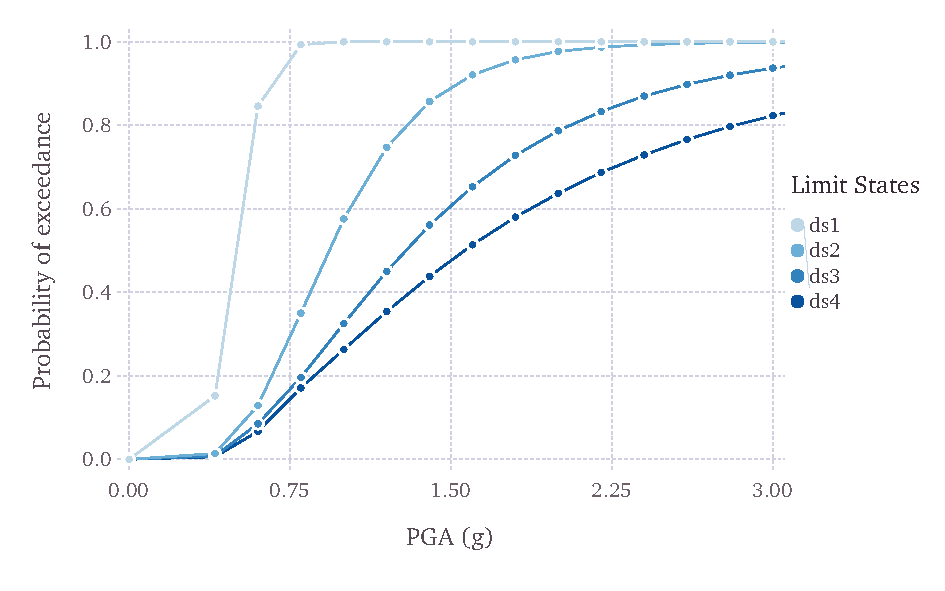
\includegraphics[width=12cm]{figures/risk/fragility-discrete.pdf}
\caption{Graphical representation of a discrete fragility model}
\label{fig:fragility-discrete}
\end{figure}

The \glspl{fragility function} can also be defined as continuous functions,
through the use of cumulative lognormal distribution functions. In
Figure~\ref{fig:fragility-continuous}, a continuous \gls{fragility model} is
presented.

\begin{figure}[ht]
\centering
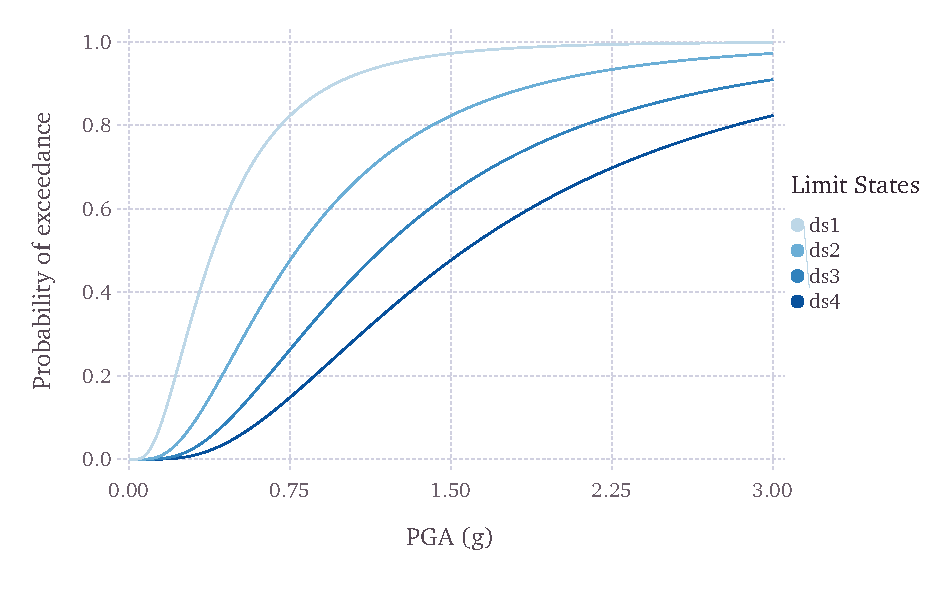
\includegraphics[width=12cm]{figures/risk/fragility-continuous.pdf}
\caption{Graphical representation of a continuous fragility model}
\label{fig:fragility-continuous}
\end{figure}

An example \gls{fragility model} comprising one discrete \gls{fragility
function} and one continuous \gls{fragility function} is shown below:

\inputminted[firstline=1,firstnumber=1,fontsize=\footnotesize,frame=single,linenos,bgcolor=lightgray]{xml}{oqum/risk/Verbatim/input_fragility.xml}\\


The initial portion of the schema contains general information that describes 
some general aspects of the \gls{fragility model}.

\begin{itemize}

    \item \Verb+id+: a unique key used to identify the \gls{fragility model}

    \item \Verb+assetCategory+: an optional string used to specify the type of
    \glspl{asset} for which \glspl{fragility function} will be defined in this
    file (e.g: buildings, lifelines)

    \item \Verb+lossCategory+: valid strings for this attribute are 
    ``structural'', ``nonstructural'', ``contents'', and 
    ``business\_interruption''

    \item \Verb+description+: a brief string with further information about the
    \gls{exposure model}

\end{itemize}

\inputminted[firstline=4,firstnumber=4,lastline=9,fontsize=\footnotesize,frame=single,linenos,bgcolor=lightgray]{xml}{oqum/risk/Verbatim/input_fragility.xml}\\

The information in the metadata section is common to all of the functions in
the \gls{fragility model} and needs to be included at the beginning of every
\gls{fragility model} file. The parameters are described below:

\begin{itemize}

    \item \Verb+description+: a brief string with further information about the
    \gls{fragility model}, for example, which building typologies are covered or 
    the source of the functions in the \gls{fragility model}

    \item \Verb+limitStates+: this field is used to define the number and 
    nomenclature of each limit state. Four limit states are employed in the 
    example above, but it is possible to use any number of discrete states,
    as long as a fragility curve is always defined for each limit state. The 
    limit states must be provided as a set of strings separated by whitespaces 
    between each limit state. Please ensure that there is no whitespace within 
    the name of any individual limit state.

\end{itemize}

In order to perform probabilistic or scenario damage calculations, it is
necessary to define a \gls{fragility function} for each building typology present in
the exposure model. The \glspl{fragility function} can be defined using either a
discrete or a continuous format, and the \gls{fragility model} file can include a
mix of both types of \glspl{fragility function}.

The following snippet from the above fragility model example file defines a
discrete fragility function:

\inputminted[firstline=11,firstnumber=11,lastline=17,fontsize=\footnotesize,frame=single,linenos,bgcolor=lightgray]{xml}{oqum/risk/Verbatim/input_fragility.xml}\\

The following attributes are needed to define a discrete \gls{fragility function}:

\begin{itemize}

    \item \Verb+id+: a unique key used to identify the \gls{taxonomy} for 
    which the function is being defined. This key is used to relate the 
    \gls{fragility function} with the relevant \gls{asset} in the 
    \gls{exposure model}.

    \item \Verb+format+: for discrete fragility functions, this attribute 
    should be set to ``\Verb+discrete+''

    \item \Verb+imls+: this attribute specifies the list of intensity levels
    for which the limit state probabilities of exceedance will be defined. 
    In addition, it is also necessary to define the intensity measure type 
    (\Verb+imt+). Optionally, a \Verb+noDamageLimit+ can be specified, which 
    defines the intensity level below which the probability of exceedance 
    for all limit states is taken to be zero.

    \item \Verb+poes+: this field is used to define the probabilities of 
    exceedance (\Verb+poes+) for each limit state for this 
    \gls{fragility function}. It is also necessary to specify which limit 
    state the exceedance probabilities are being defined for using the 
    attribute \Verb+ls+. The probabilities of exceedance for each limit state
    must be provided on a separate line; and the number of exceedance 
    probabilities for each limit state defined by the \Verb+poes+ attribute 
    must be equal to the number of intensity levels defined by the attribute 
    \Verb+imls+. Finally, the number and names of the limit states in each 
    fragility function must be equal to the number of limit states defined 
    earlier in the metadata section of the \gls{fragility model} using the 
    attribute \Verb+limitStates+.

\end{itemize}



The following snippet from the above \gls{fragility model} example file
defines a continuous \gls{fragility function}:

\inputminted[firstline=19,firstnumber=19,lastline=25,fontsize=\footnotesize,frame=single,linenos,bgcolor=lightgray]{xml}{oqum/risk/Verbatim/input_fragility.xml}\\

The following attributes are needed to define a continuous \gls{fragility function}:

\begin{itemize}

    \item \Verb+id+: a unique key used to identify the \gls{taxonomy} for 
    which the function is being defined. This key is used to relate the 
    \gls{fragility function} with the relevant \gls{asset} in the 
    \gls{exposure model}.

    \item \Verb+format+: for continuous fragility functions, this attribute 
    should be set to ``\Verb+continuous+''

    \item \Verb+shape+: for continuous fragility functions using the lognormal
    cumulative distrution, this attribute should be set to ``\Verb+logncdf+''.
    At present, only the lognormal cumulative distribution function can be 
    used for representing continuous fragility functions.

    \item \Verb+imls+: this element specifies various aspects related to the 
    intensity measure used by the the \gls{fragility function}. The range of 
    intensity levels for which the continuous fragility functions are valid 
    are specified using the attributes \Verb+minIML+ and \Verb+maxIML+. 
    In addition, it is also necessary to define the intensity measure type 
    \Verb+imt+. Optionally, a \Verb+noDamageLimit+ can be specified, which 
    defines the intensity level below which the probability of exceedance 
    for all limit states is taken to be zero.

    \item \Verb+params+: this field is used to define the parameters of the 
    continuous curve for each limit state for this 
    \gls{fragility function}. For a lognormal cumulative distrbution function, 
    the two parameters required to specify the function are the mean and 
    standard deviation of the intensity level. These parameters are defined for 
    each limit state using the attributes \Verb+mean+ and \Verb+stddev+ 
    respectively. The attribute \Verb+ls+ specifies the limit state for which 
    the parameters are being defined. The parameters for each limit state
    must be provided on a separate line. The number and names of the limit 
    states in each fragility function must be equal to the number of limit 
    states defined earlier in the metadata section of the \gls{fragility model}
    using the attribute \Verb+limitStates+.

\end{itemize}


Several methodologies to derive fragility functions are currently being
evaluated by \gls{acr:gem} and have been included as part of the Risk
Modeller's Toolkit, the code for which can be found on a public repository at
GitHub at the following address: 
\href{http://github.com/gemsciencetools/rmtk}{http://github.com/gemsciencetools/rmtk}.

Scripts to convert \glspl{fragility function} in CSV format or as Excel or
ASCII files into NRML are also under development, and can be found at the
OpenQuake platform at the following address:
\href{https://platform.openquake.org/risk_input_preparation_toolkit/}{https://platform.openquake.org/risk\_input\_preparation\_toolkit/}.


\section{Consequence Models}
\label{sec:consequence}
Starting from \glsdesc{acr:oqe17}, the Scenario Damage calculator also accepts
\glspl{consequencemodel} in addition to \glspl{fragilitymodel}, in order to
estimate consequences based on the calculated damage distribution. The user
may provide one \gls{consequencemodel} file corresponding to each loss type
(amongst structural, nonstructural, contents, and business interruption) for
which a \gls{fragilitymodel} file is provided. Whereas providing a
\gls{fragilitymodel} file for at least one loss type is mandatory for running
a Scenario Damage calculation, providing corresponding \gls{consequencemodel}
files is optional.

This section describes the schema currently used to store
\glspl{consequencemodel}, which are optional inputs for the Scenario Damage
Calculator. A \gls{consequencemodel} defines a set of
\glspl{consequencefunction}, describing the distribution of the loss (or
consequence) ratio conditional on a set of discrete limit (or damage) states.
These \gls{consequencefunction} can be currently defined in \glsdesc{acr:oqe}
by specifying the parameters of the continuous distribution of the loss ratio
for each limit state specified in the fragility model for the corresponding
loss type, for each taxonomy defined in the exposure model.

An example \gls{consequencemodel} is shown in Listing~\ref{lst:input_consequence}.

\begin{listing}[htbp]
  \inputminted[firstline=1,firstnumber=1,fontsize=\footnotesize,frame=single,linenos,bgcolor=lightgray]{xml}{oqum/risk/Verbatim/input_consequence.xml}
  \caption{Example consequence model (\href{https://raw.githubusercontent.com/GEMScienceTools/oq-engine-docs/master/oqum/risk/verbatim/input_consequence.xml}{Download example})}
  \label{lst:input_consequence}
\end{listing}	

The initial portion of the schema contains general information that describes
some general aspects of the \gls{consequencemodel}. The information in this
metadata section is common to all of the functions in the
\gls{consequencemodel} and needs to be included at the beginning of every
\gls{consequencemodel} file. The parameters are described below:

\begin{itemize}

    \item \Verb+id+: a unique string (UTF-8) used to identify the
    \gls{consequencemodel}

    \item \Verb+assetCategory+: an optional string used to specify the type of
    \glspl{asset} for which \glspl{consequencefunction} will be defined in this 
    file (e.g: buildings, lifelines)

    \item \Verb+lossCategory+: mandatory; valid strings for this attribute are 
    ``structural'', ``nonstructural'', ``contents'', and 
    ``business\_interruption''

    \item \Verb+description+: mandatory; a brief string with further 
    information about the \gls{consequencemodel}, for example, which building
    typologies are covered or the source of the functions in the
    \gls{consequencemodel}

    \item \Verb+limitStates+: mandatory; this field is used to define the number and 
    nomenclature of each limit state. Four limit states are employed in the 
    example above, but it is possible to use any number of discrete states. The 
    limit states must be provided as a set of strings separated by whitespaces 
    between each limit state. Please ensure that there is no whitespace within 
    the name of any individual limit state. The number and nomenclature of the
    limit states used in the \gls{consequencemodel} should match those used in
    the corresponding \gls{fragilitymodel}

\end{itemize}

\inputminted[firstline=4,firstnumber=4,lastline=9,fontsize=\footnotesize,frame=single,linenos,bgcolor=lightgray]{xml}{oqum/risk/Verbatim/input_consequence.xml}

The following snippet from the above \gls{consequencemodel} example file defines a
\gls{consequencefunction} using a lognormal distribution to model the uncertainty
in the consequence ratio for each limit state:

\inputminted[firstline=11,firstnumber=11,lastline=16,fontsize=\footnotesize,frame=single,linenos,bgcolor=lightgray]{xml}{oqum/risk/Verbatim/input_consequence.xml}

The following attributes are needed to define a \gls{consequencefunction}:

\begin{itemize}

    \item \Verb+id+: mandatory; a unique string (UTF-8) used to identify the \gls{taxonomy} for 
    which the function is being defined. This string is used to relate the 
    \gls{consequencefunction} with the relevant \gls{asset} in the 
    \gls{exposuremodel}.

    \item \Verb+dist+: mandatory; for vulnerability function which use a continuous 
    distribution to model the uncertainty in the conditional loss ratios, 
    this attribute should be set to either ``\Verb+LN+'' if using the lognormal
    distribution, or to ``\Verb+BT+'' if using the Beta distribution
    \footnote{Note that as of \glsdesc{acr:oqe18}, the uncertainty in the 
    consequence ratios is ignored, and only the mean consequence ratios for the
    set of limit states is considered when computing the consequences from the
    damage distribution. Consideration of the uncertainty in the consequence
    ratios will be included in future releases of the \glsdesc{acr:oqe}.}.

    \item \Verb+params+: mandatory; this field is used to define the parameters of 
    the continuous distribution used for modelling the uncertainty in the
    loss ratios for each limit state for this 
    \gls{consequencefunction}. For a lognormal distrbution, 
    the two parameters required to specify the function are the mean and 
    standard deviation of the consequence ratio. These parameters are defined for 
    each limit state using the attributes \Verb+mean+ and \Verb+stddev+ 
    respectively. The attribute \Verb+ls+ specifies the limit state for which 
    the parameters are being defined. The parameters for each limit state
    must be provided on a separate line. The number and names of the limit 
    states in each \gls{consequencefunction} must be equal to the number of limit 
    states defined in the corresponding \gls{fragilitymodel}
    using the attribute \Verb+limitStates+.

\end{itemize}

\section{Vulnerability Models}
\label{sec:vulnerability}
In order to perform probabilistic or scenario risk calculations, it is
necessary to define a \gls{vulnerabilityfunction} for each building typology
present in the \gls{exposuremodel}. In this section, the schema for the
\gls{vulnerabilitymodel} is described in detail. A graphical representation of
a \gls{vulnerabilitymodel} (mean loss ratio for a set of intensity measure
levels) is illustrated in Figure~\ref{fig:vulnerability-zero-cov}.

\begin{figure}[ht]
\centering
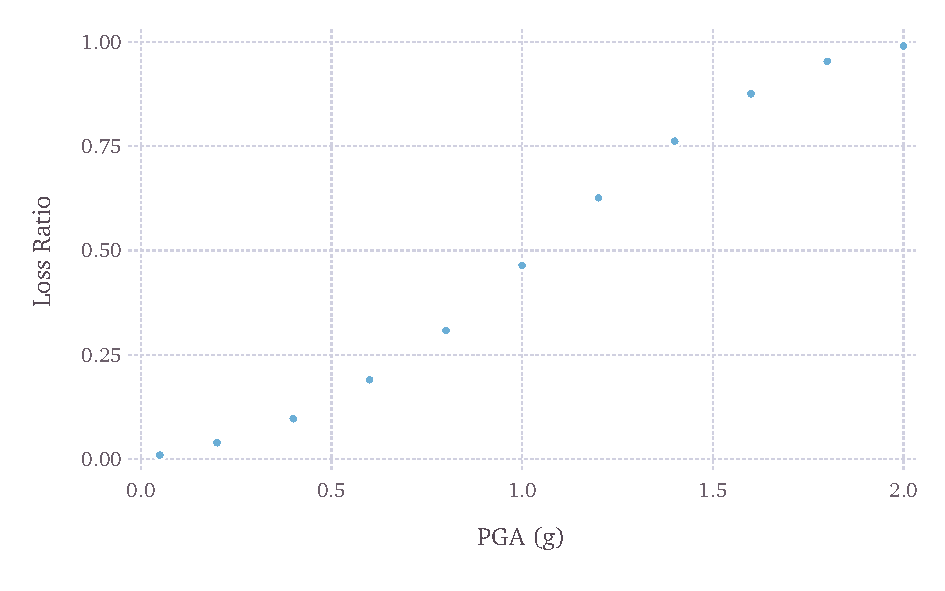
\includegraphics[width=12cm]{figures/risk/vulnerability-zero-cov.pdf}
\caption{Graphical representation of a vulnerability model}
\label{fig:vulnerability-zero-cov}
\end{figure}


Note that although the uncertainty for each loss ratio is not represented in
Figure~\ref{fig:vulnerability-zero-cov}, it can be considered in the input
file, by means of a coefficient of variation per loss ratio and a
probabilistic distribution, which can currently be set to lognormal~(LN),
Beta~(BT); or by specifying a discrete probability mass~(PM)\footnote{As of
\glsdesc{acr:oqe18}, the ``PM'' option for defining
\glspl{vulnerabilityfunction} is supported by the Scenario Risk and the
Stochastic Event-Based Probabilistic Risk Calculators, but not by the
Classical Probabilistic Risk Calculator.} distribution of the loss ratio at a
set of intensity levels. An example of a \gls{vulnerabilityfunction} that
models the uncertainty in the loss ratio at different intensity levels using a
lognormal distribution is illustrated in 
Figure~\ref{fig:vulnerability-nonzero-cov}.

\begin{figure}[ht]
\centering
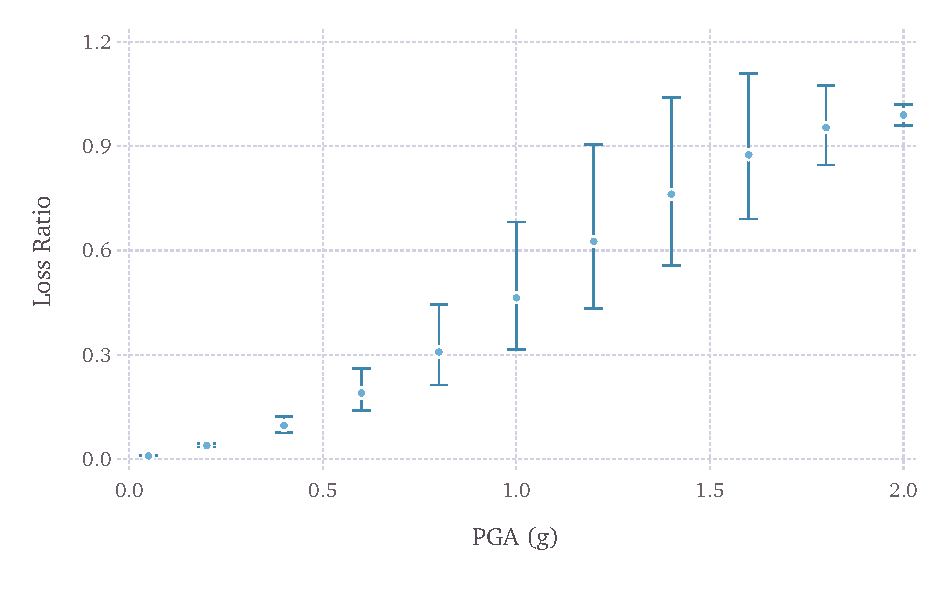
\includegraphics[width=12cm]{figures/risk/vulnerability-nonzero-cov.pdf}
\caption{Graphical representation of a vulnerability function that models the uncertainty in the loss ratio using a lognormal distribution. The mean loss ratios and coefficients of variation are illustrated for a set of intensity levels.}
\label{fig:vulnerability-nonzero-cov}
\end{figure}

In general, defining \glspl{vulnerabilityfunction} requires the user to
specify the distribution of the loss ratio for a set of intensity levels. The
loss ratio distributions can be defined using either a discrete or a
continuous format, and the \gls{vulnerabilitymodel} file can include a mix of
both types of \glspl{vulnerabilityfunction}. It is also possible to define a
\gls{vulnerabilityfunction} using a set of deterministic loss ratios
corresponding to a set of intensity levels (i.e., ignoring the uncertainty in
the conditional loss ratios).

An example \gls{vulnerabilitymodel} comprising three
\glspl{vulnerabilityfunction} is shown in
Listing~\ref{lst:input_vulnerability}. This \gls{vulnerabilitymodel} contains
one function that uses the lognormal distribution to represent the uncertainty
in the loss ratio at different intensity levels, one function that uses the
Beta distribution, and one function that is defined using a discrete
probability mass distribution.

\begin{listing}[htbp]
  \inputminted[firstline=1,firstnumber=1,fontsize=\footnotesize,frame=single,linenos,bgcolor=lightgray]{xml}{oqum/risk/Verbatim/input_vulnerability.xml}
  \caption{Example vulnerability model (\href{https://raw.githubusercontent.com/GEMScienceTools/oq-engine-docs/master/oqum/risk/verbatim/input_vulnerability.xml}{Download example})}
  \label{lst:input_vulnerability}
\end{listing}


The initial portion of the schema contains general information that describes
some general aspects of the \gls{vulnerabilitymodel}. The information in this
metadata section is common to all of the functions in the
\gls{vulnerabilitymodel} and needs to be included at the beginning of every
\gls{vulnerabilitymodel} file. The parameters are illustrated in the snippet
shown and described below:

\inputminted[firstline=4,firstnumber=4,lastline=8,fontsize=\footnotesize,frame=single,linenos,bgcolor=lightgray]{xml}{oqum/risk/Verbatim/input_vulnerability.xml}

\begin{itemize}

  \item \Verb+id+: a unique string (ASCII) used to identify the
    \gls{vulnerabilitymodel}. This string can contain letters~(a--z; A--Z),
    numbers~(0--9), dashes~(-), and underscores~(\_), with a maximum of
    100~characters.

  \item \Verb+assetCategory+: an optional string (ASCII) used to specify the
    type of \glspl{asset} for which \glspl{vulnerabilityfunction} will be 
    defined in this file (e.g: buildings, lifelines).

  \item \Verb+lossCategory+: mandatory; valid strings for this attribute are 
    ``structural'', ``nonstructural'', ``contents'',  
    ``business\_interruption'', and ``occupants''.

  \item \Verb+description+: mandatory; a brief string with further information about the
    \gls{vulnerabilitymodel}, for example, which building typologies are 
    covered or the source of the functions in the \gls{vulnerabilitymodel}.

\end{itemize}


The following snippet from the above \gls{vulnerabilitymodel} example file defines
a \gls{vulnerabilityfunction} modelling the uncertainty in the conditional loss
ratios using a (continuous) lognormal distribution:

\inputminted[firstline=10,firstnumber=10,lastline=14,fontsize=\footnotesize,frame=single,linenos,bgcolor=lightgray]{xml}{oqum/risk/Verbatim/input_vulnerability.xml}

The following attributes are needed to define a \gls{vulnerabilityfunction} which
uses a continuous distribution to model the uncertainty in the conditional
loss ratios:

\begin{itemize}

  \item \Verb+id+: a unique string (ASCII) used to identify the \gls{taxonomy} for 
    which the function is being defined. This string is used to relate the 
    \gls{vulnerabilityfunction} with the relevant \gls{asset} in the 
    \gls{exposuremodel}. This string can contain letters~(a--z; A--Z), 
    numbers~(0--9), dashes~(-), and underscores~(\_), with a maximum of
    100~characters.

  \item \Verb+dist+: mandatory; for \glspl{vulnerabilityfunction} which use a continuous 
    distribution to model the uncertainty in the conditional loss ratios, 
    this attribute should be set to either ``\Verb+LN+'' if using the lognormal
    distribution, or to ``\Verb+BT+'' if using the Beta distribution.

  \item \Verb+imls+: mandatory; this attribute specifies the list of intensity levels
    for which the parameters of the conditional loss ratio distributions will
    be defined. In addition, it is also necessary to define the intensity 
    measure type (\Verb+imt+).

  \item \Verb+meanLRs+: mandatory; this field is used to define the mean loss ratios
    for this \gls{vulnerabilityfunction} for each of the intensity levels
    defined by the attribute \Verb+imls+. The number of mean loss ratios
    defined by the \Verb+meanLRs+ attribute must be equal to the number of
    intensity levels defined by the attribute \Verb+imls+.

  \item \Verb+covLRs+: mandatory; this field is used to define the coefficient of 
    variation for the conditional distribution of the loss ratios for this
    \gls{vulnerabilityfunction} for each of the intensity levels defined by
    the attribute \Verb+imls+. The number of coefficients of variation of loss
    ratios defined by the \Verb+covLRs+ attribute must be equal to the number
    of intensity levels defined by the attribute \Verb+imls+. The uncertainty
    in the conditional loss ratios can be ignored by setting all of the
    \Verb+covLRs+ for a given \gls{vulnerabilityfunction} to zero.

\end{itemize}


The next snippet from the \gls{vulnerabilitymodel} example file of
Listing~\ref{lst:input_vulnerability} defines a \gls{vulnerabilityfunction}
which models the uncertainty in the conditional loss ratios using a
(discrete) probability mass distribution:

\inputminted[firstline=24,firstnumber=24,lastline=33,fontsize=\footnotesize,frame=single,linenos,bgcolor=lightgray]{xml}{oqum/risk/Verbatim/input_vulnerability.xml}

The following attributes are needed to define a \gls{vulnerabilityfunction}
which uses a discrete probability mass distribution to model the uncertainty
in the conditional loss ratios:

\begin{itemize}

  \item \Verb+id+: a unique string (ASCII) used to identify the \gls{taxonomy} for 
    which the function is being defined. This string is used to relate the 
    \gls{vulnerabilityfunction} with the relevant \gls{asset} in the 
    \gls{exposuremodel}. This string can contain letters~(a--z; A--Z), 
    numbers~(0--9), dashes~(-), and underscores~(\_), with a maximum of
    100~characters.

  \item \Verb+dist+: mandatory; for \glspl{vulnerabilityfunction} which use a 
    discrete probability mass distribution to model the uncertainty in the
    conditional loss ratios, this attribute should be set to ``\Verb+PM+''.

  \item \Verb+imls+: mandatory; this attribute specifies the list of intensity levels
    for which the parameters of the conditional loss ratio distributions will
    be defined. In addition, it is also necessary to define the intensity 
    measure type (\Verb+imt+).

  \item \Verb+probabilities+: mandatory; this field is used to define the
    probability of observing a particular loss ratio (specified for each row of
    \Verb+probabilities+ using the attribute \Verb+lr+), conditional on the set
    of intensity levels specified using the attribute \Verb+imls+.
    for this \gls{vulnerabilityfunction}. Thus, the number of probabilities
    defined by each \Verb+probabilities+ attribute must be equal to the number
    of intensity levels defined by the attribute \Verb+imls+. On the other hand,
    there is no limit to the number of loss ratios for which
    \Verb+probabilities+ can be defined. In the example shown here, notice that
    the set of probabilities conditional on any particular intensity level,
    say, $MMI = 8$, sum up to one.

\end{itemize}


Note that the schema for representing \glspl{vulnerabilitymodel} has changed
between \gls{acr:nrml} v0.4 (used prior to \gls{acr:oqe17}) and \gls{acr:nrml}
v0.5 (introduced in \gls{acr:oqe17}).

A deprecation warning is printed every time you attempt to use a
\gls{vulnerabilitymodel} in the old \gls{acr:nrml} v0.4 format in an
\gls{acr:oqe17} (or later) risk calculation. To get rid of the warning you
must upgrade the old \glspl{vulnerabilitymodel} files to \gls{acr:nrml} v0.5.
You can use the command \Verb+upgrade_nrml+ with oq-lite to do this as
follows:

\begin{minted}[fontsize=\footnotesize,frame=single,bgcolor=lightgray]{shell-session}
user@ubuntu:~\$ oq-lite upgrade_nrml <directory-name>
\end{minted}

The above command will upgrade all of your old \gls{vulnerabilitymodel} files to
\gls{acr:nrml} v0.5. The original files will be kept, but with a .bak extension
appended. Notice that you will need to set the \Verb+lossCategory+ attribute
to its correct value manually. This is easy to do, since if you try to run a
computation you will get a clear error message telling the expected value for
the \Verb+lossCategory+ for each file.


Several methodologies to derive \glspl{vulnerabilityfunction} are currently being
evaluated by \gls{acr:gem} and have been included as part of the Risk
Modeller's Toolkit, the code for which can be found on a public repository at
GitHub at: 
\href{http://github.com/gemsciencetools/rmtk}{http://github.com/gemsciencetools/rmtk}.

A web-based tool to build an \gls{vulnerabilitymodel} in the \gls{acr:nrml} schema
are also under development, and can be found at the OpenQuake platform at the
following address: \href{https://platform.openquake.org/ipt/}{https://platform.openquake.org/ipt/}.

   \cleardoublepage

\chapterimage{figures/chapter_head.pdf} % Chapter heading image
\chapter{Using the Risk Module}
	\label{chap:riskcalculators}
	This Chapter summarises the structure of the information necessary to define
the different input data to be used with the OpenQuake-engine risk
calculators. Input data for scenario-based and probabilistic seismic damage
and risk analysis using OpenQuake-engine are organised into:

\begin{itemize}

  \item An exposure model file in the NRML format, as described in 
    Section~\ref{sec:exposure}.

  \item A file describing the \gls{vulnerability model}
    (Section~\ref{sec:vulnerability}) for loss calculations, or a 
  	file describing the \gls{fragility model} (Section~\ref{sec:fragility})
    for damage calculations. Optionally, a file describing the
    \gls{consequence model} (Section~\ref{sec:consequence}) can also be
  	provided in order to calculate losses from the estimated damage
  	distributions.

  \item A general calculation configuration file.

  \item Hazard inputs. These include hazard curves for the classical
    probabilistic damage and risk calculators, ground motion fields for the
    scenario damage and risk calculators, or stochastic event sets for the
    probabilistic event based calculators. As of OpenQuake-engine v1.6, in
    general, there are five different ways in which hazard calculation
    parameters or results can be provided to the OpenQuake-engine in order to
    run the subsequent risk calculations:

    \begin{itemize}

      \item Use a single configuration file for running the hazard and risk
      calculations sequentially

      \item Use separate configuration files for running the hazard and risk
      calculations sequentially

      \item Use a configuration file for the risk calculation along with all
      hazard outputs from a previously completed, compatible
      OpenQuake-engine hazard calculation

      \item Use a configuration file for the risk calculation along with a
      specific hazard output from a previously completed, compatible
      OpenQuake-engine hazard calculation

      \item Use a configuration file for the risk calculation along with
      hazard input files in the OpenQuake NRML format

    \end{itemize}

\end{itemize}

The file formats for exposure, fragility, consequence, and vulnerability
models have been described earlier in Chapter~\ref{chap:riskintro}. The
configuration file is the primary file that provides the OpenQuake-engine
information regarding both the definition of the input models (e.g. exposure,
site parameters, fragility, consequence, or vulnerability models) as well as
the parameters governing the risk calculation.

Information regarding the configuration file for running hazard calculations
using OpenQuake-engine can be found in
Section~\ref{sec:hazard_configuration_file}. Some initial parameters of the
configuration file common to all of the risk calculators are presented below.
The remaining parameters that are specific to each risk calculator are
discussed in subsequent sections.

\inputminted[firstline=1,firstnumber=1,fontsize=\footnotesize,frame=single,linenos,bgcolor=lightgray]{ini}{oqum/risk/Verbatim/config_example.ini}\\

\begin{itemize}

  \item \Verb+description+: a parameter that can be used to include some
  information about the type of calculations that are going to be performed.

  \item \Verb+calculation_mode+: this parameter specifies the type of
  calculation to be run. Valid options for the \Verb+calculation_mode+ for
  the risk calculators are: \Verb+scenario_damage+, \Verb+scenario_risk+,
  \Verb+classical_damage+, \Verb+classical_risk+, \Verb+event_based_risk+,
  and \Verb+classical_bcr+.

  \item \Verb+exposure_file+: this parameter is used to specify the path to
  the \gls{exposure model} file.

\end{itemize}

Depending on the type of risk calculation, other parameters besides the
aforementioned ones may need to be provided. We illustrate in the following
sections different examples of the configuration file for the different risk
calculators.


\section{Scenario Damage Calculator}
\label{sec:config_scenario_damage}
For this calculator, the parameter \Verb+calculation_mode+ should be set to
\Verb+scenario_damage+.

\paragraph{Example 1}

This example illustrates a scenario damage calculation which uses a single
configuration file to first compute the ground motion fields for the given
rupture model and then calculate damage distribution statistics based on the
ground motion fields. A minimal job configuration file required for running a
scenario damage calculation is shown in
Listing~\ref{lst:config_scenario_damage_combined}.

\begin{listing}[htbp]
  \inputminted[firstline=1,firstnumber=1,fontsize=\footnotesize,frame=single,linenos,bgcolor=lightgray,label=job.ini]{ini}{oqum/risk/verbatim/config_scenario_damage_combined.ini}
  \caption{Example combined configuration file for running a scenario damage calculation (\href{https://raw.githubusercontent.com/GEMScienceTools/oq-engine-docs/master/oqum/risk/verbatim/config_scenario_damage_combined.xml}{Download example})}
  \label{lst:config_scenario_damage_combined}
\end{listing}

The general parameters \Verb+description+ and \Verb+calculation_mode+, and
\Verb+exposure_file+ have already been described earlier. The other parameters
seen in the above example configuration file are described below:

\begin{itemize}

  \item \Verb+rupture_model_file+: a parameter used to define the path
	to the earthquake \gls{rupturemodel} file describing the scenario event.

  \item \Verb+rupture_mesh_spacing+: a parameter used to specify the mesh size
  	(in km) used by the \glsdesc{acr:oqe} to discretize the rupture.
  	Note that the smaller the mesh spacing, the greater will be
  	(1) the precision in the calculation and
  	(2) the computational demand.

  \item \Verb+structural_fragility_file+: a parameter used to define the path
	to the structural \gls{fragilitymodel} file.

\end{itemize}

In this case, the ground motion fields will be computed at each of the
locations of the assets in the exposure model. Ground motion fields will be
generated for each of the intensity measure types found in the provided set of
fragility models. The above calculation can be run using the command line:

\begin{minted}[fontsize=\footnotesize,frame=single,bgcolor=lightgray]{shell-session}
user@ubuntu:~\$ oq-engine --run job.ini
\end{minted}

After the calculation is completed, a message similar to the following will be
displayed:

\begin{minted}[fontsize=\footnotesize,frame=single,bgcolor=lightgray]{shell-session}
Calculation 2680 completed in 13 seconds. Results:
  id | output_type | name
5069 | datastore   | dmg_by_asset_and_collapse_map
5070 | datastore   | dmg_by_taxon
5071 | datastore   | dmg_total
\end{minted}

Note that one or more of the following parameters can be used in the same job
configuration file to provide the corresponding fragility model files:

\begin{itemize}

  \item \Verb+structural_fragility_file+: a parameter used to define the path
    to a structural \gls{fragilitymodel} file

  \item \Verb+nonstructural_fragility_file+: a parameter used to define the path
    to a nonstructural \gls{fragilitymodel} file

  \item \Verb+contents_fragility_file+: a parameter used to define the path
    to a contents \gls{fragilitymodel} file

  \item \Verb+business_interruption_fragility_file+: a parameter used to define
    the path to a business interruption \gls{fragilitymodel} file

\end{itemize}

It is important that the \Verb+lossCategory+ parameter in the metadata section
for each provided fragility model file (``structural'', ``nonstructural'',
``contents'', or ``business\_interruption'') should match the loss type
defined in the configuration file by the relevant keyword above.


\paragraph{Example 2}

This example illustrates a scenario damage calculation which uses separate
configuration files for the hazard and risk parts of a scenario damage
assessment. The first configuration file shown in
Listing~\ref{lst:config_scenario_damage_hazard} contains input models and
parameters required for the computation of the ground motion fields due to a
given rupture. The second configuration file shown in
Listing~\ref{lst:config_scenario_damage} contains input models and parameters
required for the calculation of the damage distribution for a portfolio of
assets due to the ground motion fields.

\begin{listing}[htbp]
  \inputminted[firstline=1,firstnumber=1,fontsize=\footnotesize,frame=single,linenos,bgcolor=lightgray,label=job\_hazard.ini]{ini}{oqum/risk/verbatim/config_scenario_hazard.ini}
  \caption{Example hazard configuration file for a scenario damage calculation (\href{https://raw.githubusercontent.com/GEMScienceTools/oq-engine-docs/master/oqum/risk/verbatim/config_scenario_hazard.xml}{Download example})}
  \label{lst:config_scenario_damage_hazard}
\end{listing}

\begin{listing}[htbp]
  \inputminted[firstline=1,firstnumber=1,fontsize=\footnotesize,frame=single,linenos,bgcolor=lightgray,label=job\_damage.ini]{ini}{oqum/risk/verbatim/config_scenario_damage.ini}
  \caption{Example risk configuration file for a scenario damage calculation (\href{https://raw.githubusercontent.com/GEMScienceTools/oq-engine-docs/master/oqum/risk/verbatim/config_scenario_damage.xml}{Download example})}
  \label{lst:config_scenario_damage}
\end{listing}


In this example, the set of intensity measure types for which the ground
motion fields should be generated is specified explicitly in the configuration
file using the parameter \Verb+intensity_measure_types+. If the hazard
calculation outputs are intended to be used as inputs for a subsequent
scenario damage or risk calculation, the set of intensity measure types
specified here must include all intensity measure types that are used in the
fragility or vulnerability models for the subsequent damage or risk
calculation.

In the hazard configuration file illustrated above
(Listing~\ref{lst:config_scenario_damage_hazard}), the list of sites at which
the ground motion values will be computed is provided in a CSV file, specified
using the \Verb+sites_csv+ parameter. The sites used for the hazard
calculation need not be the same as the locations of the assets in the
exposure model used for the following risk calculation. In such cases, it is
recommended to set a reasonable search radius (in km) using the
\Verb+asset_hazard_distance+ parameter for the \glsdesc{acr:oqe} to look for
available hazard values, as shown in the job\_damage.ini example file above.

The only new parameters introduced in risk configuration file for this example
(Listing~\ref{lst:config_scenario_damage}) are the \Verb+region_constraint+
and \Verb+asset_hazard_distance+ parameters, which are described below; all
other parameters have already been described in earlier examples.

\begin{itemize}

  \item \Verb+region_constraint+: this is an optional parameter, applicable
    only to risk calculations, which defines the polygon that will be used for
    filtering the assets from the exposure model. Assets outside of this region
    will not be considered in the risk calculations. This region is defined
    using pairs of coordinates that indicate the vertices of the polygon, which
    should be listed in the Well-known text (WKT) format:

    region\_constraint = lon\_1 lat\_1, lon\_2 lat\_2, ..., lon\_n lat\_n

    For each point, the longitude is listed first, followed by the latitude,
    both in decimal degrees. The list of points defining the polygon can be
    provided either in a clockwise or counter-clockwise direction.

    If the \Verb+region_constraint+ is not provided, all assets in the exposure
    model are considered for the risk calculation.

    This parameter is useful in cases where the exposure model covers a region
    larger than the one that is of interest in the current calculation.

  \item \Verb+asset_hazard_distance+: this parameter indicates the maximum
    allowable distance between an \gls{asset} and the closest hazard input.
    Hazard inputs can include hazard curves or ground motion intensity values.
    If no hazard input site is found within the radius defined by the
    \Verb+asset_hazard_distance+, the asset is skipped and a message is
    provided mentioning the id of the asset that is affected by this issue.

    If multiple hazard input sites are found within the radius defined by the
    this parameter, the hazard input site with the shortest distance from the
    asset location is associated with the asset. It is possible that the
    associated hazard input site might be located outside the polygon defined
    by the \Verb+region_constraint+.

\end{itemize}


Now, the above calculations described by the two configuration files
``job\_hazard.ini'' and ``job\_damage.ini'' can be run sequentially using the
command line as follows:

\begin{minted}[fontsize=\footnotesize,frame=single,bgcolor=lightgray]{shell-session}
user@ubuntu:~\$ oq-engine --run job_hazard.ini,job_damage.ini
\end{minted}

The hazard and risk calculations can also be run separately. In that case, the
calculation id for the hazard calculation or the output id for the specific
ground motion fields output generated by the hazard calculation should be
provided to the \glsdesc{acr:oqe} while running the risk calculation using the
options \Verb+--hazard-calculation-id+ (or \Verb+--hc+) and 
\Verb+--hazard-output-id+ (or \Verb+--ho+) respectively. This is shown below:

\begin{minted}[fontsize=\footnotesize,frame=single,bgcolor=lightgray]{shell-session}
user@ubuntu:~\$ oq-engine --run job_hazard.ini
\end{minted}

After the hazard calculation is completed, a message similar to the one below
will be displayed in the terminal:

\begin{minted}[fontsize=\footnotesize,frame=single,bgcolor=lightgray]{shell-session}
Calculation 2681 completed in 4 seconds. Results:
  id | output_type | name
5072 | datastore   | gmfs
\end{minted}

In the example above, the calculation~id of the hazard calculation is 2681.
There is only one output from this calculation, i.e., the \glspl{acr:gmf}. The
output~id for the \glspl{acr:gmf} generated by the above calculation is 5072.

The risk calculation for computing the damage distribution statistics for the
portfolio of \glspl{asset} can now be run using either:

\begin{minted}[fontsize=\footnotesize,frame=single,bgcolor=lightgray]{shell-session}
user@ubuntu:~\$ oq-engine --run job_damage.ini --hc 2681
\end{minted}

or

\begin{minted}[fontsize=\footnotesize,frame=single,bgcolor=lightgray]{shell-session}
user@ubuntu:~\$ oq-engine --run job_damage.ini --ho 5072
\end{minted}

After the calculation is completed, a message similar to the one listed above
in Example~1 will be displayed.

In order to retrieve the calculation~id of a previously run hazard calculation,
the option \Verb+--list-hazard-calculations+ (or \Verb+--lhc+) can be used to
display a list of all previously run hazard calculations:

\begin{minted}[fontsize=\footnotesize,frame=single,bgcolor=lightgray]{shell-session}
job_id |     status |         last_update |         description
  2609 | successful | 2015-12-01 14:14:14 | Mid Nepal earthquake
  ...
  2681 | successful | 2015-12-12 10:00:00 | Scenario hazard example
\end{minted}

The option \Verb+--list-outputs+ (or \Verb+--lo+) can be used to display a
list of all outputs generated during a particular calculation. For instance,

\begin{minted}[fontsize=\footnotesize,frame=single,bgcolor=lightgray]{shell-session}
user@ubuntu:~\$ oq-engine --lo 2681
\end{minted}

will produce the following display:

\begin{minted}[fontsize=\footnotesize,frame=single,bgcolor=lightgray]{shell-session}
  id | output_type | name
5072 | datastore   | gmfs
\end{minted}


\paragraph{Example 3}

The example shown in Listing~\ref{lst:config_scenario_damage_gmf} illustrates
a scenario damage calculation which uses a file listing a precomputed set of
\glspl{acr:gmf}. These \glspl{acr:gmf} can be computed using the
\glsdesc{acr:oqe} or some other software. The \glspl{acr:gmf} must be provided
in the \gls{acr:nrml} schema as presented in
Section~\ref{subsec:output_event_based_psha}. The damage distribution is
computed based on the provided \glspl{acr:gmf}.

\begin{listing}[htbp]
  \inputminted[firstline=1,firstnumber=1,fontsize=\footnotesize,frame=single,linenos,bgcolor=lightgray,label=job.ini]{ini}{oqum/risk/verbatim/config_scenario_damage_gmf.ini}
  \caption{Example configuration file for a scenario damage calculation using a precomputed set of ground motion fields (\href{https://raw.githubusercontent.com/GEMScienceTools/oq-engine-docs/master/oqum/risk/verbatim/config_scenario_damage_gmf.xml}{Download example})}
  \label{lst:config_scenario_damage_gmf}
\end{listing}

\begin{itemize}

  \item \Verb+gmfs_file+: a parameter used to define the path
	  to the \glspl{acr:gmf} file in the \gls{acr:nrml} schema. This file must
    define \glspl{acr:gmf} for all of the intensity measure types used in the
    \gls{fragilitymodel}.

\end{itemize}

The above calculation can be run using the command line:

\begin{minted}[fontsize=\footnotesize,frame=single,bgcolor=lightgray]{shell-session}
user@ubuntu:~\$ oq-engine --run job.ini
\end{minted}


\paragraph{Example 4}

This example illustrates a the hazard job configuration file for a scenario
damage calculation which uses two \glspl{acr:gmpe} instead of only one.
Currently, the set of \glspl{acr:gmpe} to be used for a scenario calculation
can be specified using a logic tree file, as demonstrated in
\ref{subsec:gmlt}. As of \glsdesc{acr:oqe18}, the weights in the logic tree
are ignored, and a set of \glspl{acr:gmf} will be generated for each
\gls{acr:gmpe} in the logic tree file. Correspondingly, damage distribution
statistics will be generated for each set of \gls{acr:gmf}.

The file shown in Listing~\ref{lst:input_scenario_gmlt} lists the two
\glspl{acr:gmpe} to be used for the hazard calculation:

\begin{listing}[htbp]
  \inputminted[firstline=1,firstnumber=1,fontsize=\footnotesize,frame=single,linenos,bgcolor=lightgray,label=gsim\_logic\_tree.xml]{xml}{oqum/risk/verbatim/input_scenario_gmlt.xml}
  \caption{Example ground motion logic tree for a scenario calculation (\href{https://raw.githubusercontent.com/GEMScienceTools/oq-engine-docs/master/oqum/risk/verbatim/input_scenario_gmlt.xml}{Download example})}
  \label{lst:input_scenario_gmlt}
\end{listing}

The only change that needs to be made in the hazard job configuration file is
to replace the \Verb+gsim+ parameter with \Verb+gsim_logic_tree_file+, as
demonstrated in Listing~\ref{lst:config_scenario_hazard_gmlt}.

\begin{listing}[htbp]
  \inputminted[firstline=1,firstnumber=1,fontsize=\footnotesize,frame=single,linenos,bgcolor=lightgray,label=job\_hazard.ini]{ini}{oqum/risk/verbatim/config_scenario_hazard_gmlt.ini}
  \caption{Example configuration file for a scenario damage calculation using a logic-tree file (\href{https://raw.githubusercontent.com/GEMScienceTools/oq-engine-docs/master/oqum/risk/verbatim/config_scenario_hazard_gmlt.xml}{Download example})}
  \label{lst:config_scenario_hazard_gmlt}
\end{listing}


\paragraph{Example 5}

This example illustrates a scenario damage calculation which specifies
fragility models for calculating damage to structural and nonstructural
components of structures, and also specifies \gls{consequencemodel} files for
calculation of the corresponding losses.

A minimal job configuration file required for running a scenario damage
calculation followed by a consequences analysis is shown in
Listing~\ref{lst:config_scenario_damage_consequences}.

\begin{listing}[htbp]
  \inputminted[firstline=1,firstnumber=1,fontsize=\footnotesize,frame=single,linenos,bgcolor=lightgray,label=job.ini]{ini}{oqum/risk/verbatim/config_scenario_damage_consequences.ini}
  \caption{Example configuration file for a scenario damage calculation followed by a consequences analysis (\href{https://raw.githubusercontent.com/GEMScienceTools/oq-engine-docs/master/oqum/risk/verbatim/config_scenario_damage_consequences.xml}{Download example})}
  \label{lst:config_scenario_damage_consequences}
\end{listing}

Note that one or more of the following parameters can be used in the same job
configuration file to provide the corresponding \gls{consequencemodel} files:

\begin{itemize}

  \item \Verb+structural_consequence_file+: a parameter used to define the path
    to a structural \gls{consequencemodel} file

  \item \Verb+nonstructural_consequence_file+: a parameter used to define the path
    to a nonstructural \gls{consequencemodel} file

  \item \Verb+contents_consequence_file+: a parameter used to define the path
    to a contents \gls{consequencemodel} file

  \item \Verb+business_interruption_consequence_file+: a parameter used to define
    the path to a business interruption \gls{consequencemodel} file

\end{itemize}

It is important that the \Verb+lossCategory+ parameter in the metadata section
for each provided \gls{consequencemodel} file (``structural'', ``nonstructural'',
``contents'', or ``business\_interruption'') should match the loss type
defined in the configuration file by the relevant keyword above.

The above calculation can be run using the command line:

\begin{minted}[fontsize=\footnotesize,frame=single,bgcolor=lightgray]{shell-session}
user@ubuntu:~\$ oq-engine --run job.ini
\end{minted}

After the calculation is completed, a message similar to the following will be
displayed:

\begin{minted}[fontsize=\footnotesize,frame=single,bgcolor=lightgray]{shell-session}
Calculation 1579 completed in 37 seconds. Results:
  id | output_type | name
8990 | datastore | csq_by_asset
8991 | datastore | csq_by_taxon
8992 | datastore | csq_total
8993 | datastore | dmg_by_asset_and_collapse_map
8994 | datastore | dmg_by_taxon
8995 | datastore | dmg_total
\end{minted}


\section{Scenario Risk Calculator}
\label{sec:config_scenario_risk}
In order to run this calculator, the parameter \Verb+calculation_mode+ needs
to be set to \Verb+scenario_risk+. 

Most of the job configuration parameters required for running a scenario risk
calculation are the same as those described in the previous section for the
scenario damage calculator. The remaining parameters specific to the scenario
risk calculator are illustrated through the example below.


\paragraph{Example 1}

This example illustrates a scenario risk calculation which uses a single
configuration file to first compute the ground motion fields for the given
rupture model and then calculate loss statistics for structural losses,
nonstructural losses, and insured structural losses, based on the ground
motion fields. The job configuration file required for running this scenario
risk calculation is shown below:

\inputminted[firstline=1,firstnumber=1,fontsize=\footnotesize,frame=single,linenos,bgcolor=lightgray,label=job.ini]{ini}{oqum/risk/verbatim/config_scenario_risk_combined.ini}\\

Whereas a scenario damage calculation requires one or more fragility and/or
consequence models, a scenario risk calculation requires the user to specify
one or more vulnerability model files. Note that one or more of the following
parameters can be used in the same job configuration file to provide the
corresponding vulnerability model files:

\begin{itemize}

  \item \Verb+structural_vulnerability_file+: this parameter is used to
    specify the path to the structural \gls{vulnerability model} file

  \item \Verb+nonstructural_vulnerability_file+: this parameter is used to
    specify the path to the nonstructural\gls{vulnerability model} file

  \item \Verb+contents_vulnerability_file +: this parameter is used to
    specify the path to the contents \gls{vulnerability model} file

  \item \Verb+business_interruption_vulnerability_file +: this parameter is
    used to specify the path to the business interruption
    \gls{vulnerability model} file

  \item \Verb+occupants_vulnerability_file+: this parameter is used to
    specify the path to the occupants \gls{vulnerability model} file

\end{itemize}

It is important that the \Verb+lossCategory+ parameter in the metadata section
for each provided vulnerability model file (``structural'', ``nonstructural'',
``contents'', ``business\_interruption'', or ``occupants'') should match the
loss type defined in the configuration file by the relevant keyword above.

The remaining new parameters introduced in this example are the following:

\begin{itemize}

  \item \Verb+master_seed+: this parameter is used to control the random
    number generator in the loss ratio sampling process. If the same
    \Verb+master_seed+ is defined at each calculation run, the same random loss
    ratios will be generated, thus allowing reproducibility of the results.

  \item \Verb+asset_correlation+: if the uncertainty in the loss ratios
    has been defined within the \gls{vulnerability model}, users can specify
    a coefficient of correlation that will be used in the Monte Carlo sampling
    process of the loss ratios, between the assets that share the same
    \gls{taxonomy}. If the \texttt{asset\_correlation} is set to one,
    the loss ratio residuals will be perfectly correlated. On the other hand,
    if this parameter is set to zero, the loss ratios will be sampled
    independently. Any value between zero and one will lead to increasing
    levels of correlation. If this parameter is not defined, the
    OpenQuake-engine will assume zero correlation in the vulnerability.

  \item \Verb+insured_losses+: this parameter specifies whether insured losses
    should be calculated; the default value of this parameter is \Verb+false+.
    In order for the OpenQuake-engine to be able to compute insured losses, the
    insurance limits and deductibles must be listed for each asset in the 
    exposure model, as described in Example~5 in \ref{sec:exposure}.

\end{itemize}

In this case, the ground motion fields will be computed at each of the
locations of the assets in the exposure model and for each of the intensity
measure types found in the provided set of vulnerability models. The above
calculation can be run using the command line:

\begin{Verbatim}[frame=single, commandchars=\\\{\}, samepage=true]
user@ubuntu:~\$ oq-engine --run job.ini
\end{Verbatim}

After the calculation is completed, a message similar to the following will be
displayed:

\begin{Verbatim}[frame=single, commandchars=\\\{\}, samepage=true]
Calculation 2735 completed in 10 seconds. Results:
  id | output_type | name
5328 | datastore | agglosses-rlzs
5329 | datastore | loss_map-rlzs
\end{Verbatim}


All of the different ways of running a scenario damage calculation as
illustrated through the examples of the previous section are also applicable
to the scenario risk calculator, though the examples are not repeated here.


\section{Classical Probabilistic Seismic Damage Calculator}
\label{sec:config_classical_damage}
In order to run this calculator, the parameter \Verb+calculation_mode+ needs
to be set to \Verb+classical_damage+.

Most of the job configuration parameters required for running a classical
probabilistic damage calculation are the same as those described in the
section for the scenario damage calculator. The remaining parameters specific
to the classical probabilistic damage calculator are illustrated through the
examples below.

\paragraph{Example 1}

This example illustrates a classical probabilistic damage calculation which
uses a single configuration file to first compute the hazard curves for the
given source model and ground motion model and then calculate damage
distribution statistics based on the hazard curves. A minimal job
configuration file required for running a classical probabilistic damage
calculation is shown in Listing~\ref{lst:config_classical_damage_combined}.

\begin{listing}[htbp]
  \inputminted[firstline=1,firstnumber=1,fontsize=\footnotesize,frame=single,linenos,bgcolor=lightgray,label=job.ini]{ini}{oqum/risk/verbatim/config_classical_damage_combined.ini}
  \caption{Example combined configuration file for a classical probabilistic damage calculation (\href{https://raw.githubusercontent.com/GEMScienceTools/oq-engine-docs/master/oqum/risk/verbatim/config_classical_damage_combined.ini}{Download example})}
  \label{lst:config_classical_damage_combined}
\end{listing}

The general parameters \Verb+description+ and \Verb+calculation_mode+, and
\Verb+exposure_file+ have already been described earlier in
Section~\ref{sec:config_scenario_damage}. The parameters related to the
hazard curves computation have been described earlier in
Section~\ref{subsec:config_classical_psha}.

In this case, the hazard curves will be computed at each of the locations of
the assets in the exposure model, for each of the intensity measure types
found in the provided set of \glspl{fragilitymodel}. The above calculation can be
run using the command line:

\begin{minted}[fontsize=\footnotesize,frame=single,bgcolor=lightgray]{shell-session}
user@ubuntu:~\$ oq engine --run job.ini
\end{minted}

After the calculation is completed, a message similar to the following will be
displayed:

\begin{minted}[fontsize=\footnotesize,frame=single,bgcolor=lightgray]{shell-session}
Calculation 2741 completed in 12 seconds. Results:
  id | name
5359 | damages-rlzs
\end{minted}


\paragraph{Example 2}

This example illustrates a classical probabilistic damage calculation which
uses separate configuration files for the hazard and risk parts of a classical
probabilistic damage assessment. The first configuration file shown in
Listing~\ref{lst:config_classical_damage_hazard} contains input models and parameters
required for the computation of the hazard curves. The second configuration
file shown in Listing~\ref{lst:config_classical_damage} contains input models
and parameters required for the calculation of the probabilistic damage
distribution for a portfolio of assets based on the hazard curves and
fragility models.

\begin{listing}[htbp]
  \inputminted[firstline=1,firstnumber=1,fontsize=\footnotesize,frame=single,linenos,bgcolor=lightgray,label=job\_hazard.ini]{ini}{oqum/risk/verbatim/config_classical_hazard.ini}
  \caption{Example hazard configuration file for a classical probabilistic damage calculation (\href{https://raw.githubusercontent.com/GEMScienceTools/oq-engine-docs/master/oqum/risk/verbatim/config_classical_hazard.ini}{Download example})}
  \label{lst:config_classical_damage_hazard}
\end{listing}

\begin{listing}[htbp]
  \inputminted[firstline=1,firstnumber=1,fontsize=\footnotesize,frame=single,linenos,bgcolor=lightgray,label=job\_damage.ini]{ini}{oqum/risk/verbatim/config_classical_damage.ini}
  \caption{Example risk configuration file for a classical probabilistic damage calculation (\href{https://raw.githubusercontent.com/GEMScienceTools/oq-engine-docs/master/oqum/risk/verbatim/config_classical_damage.ini}{Download example})}
  \label{lst:config_classical_damage}
\end{listing}

Now, the above calculations described by the two configuration files
``job\_hazard.ini'' and ``job\_damage.ini'' can be run sequentially or
separately, as illustrated in Example~2 in
Section~\ref{sec:config_scenario_damage}. The new parameters introduced in the
above example configuration file are described below:

\begin{itemize}

  \item \Verb+risk_investigation_time+: an optional parameter that can be used
    in probabilistic damage or risk calculations where the period of interest
    for the risk calculation is different from the period of interest for the 
    hazard calculation. If this parameter is not explicitly set, the 
    \glsdesc{acr:oqe} will assume that the risk calculation is over the same 
    time period as the preceding hazard calculation.

  \item \Verb+steps_per_interval+: an optional parameter that can be used to
    specify whether discrete fragility functions in the fragility models should
    be discretized further, and if so, how many intermediate steps to use for
    the discretization. Setting 

    steps\_per\_interval = n

    will result in the \glsdesc{acr:oqe} discretizing the discrete fragility
    models using (n - 1) linear interpolation steps between each pair of 
    {intensity level, poe} points.

    The default value of this parameter is one, implying no interpolation.

\end{itemize}


\section{Classical Probabilistic Seismic Risk Calculator}
\label{sec:config_classical_risk}
In order to run this calculator, the parameter \Verb+calculation_mode+ needs
to be set to \Verb+classical_risk+.

Most of the job configuration parameters required for running a classical
probabilistic risk calculation are the same as those described in the previous
section for the classical probabilistic damage calculator. The remaining
parameters specific to the classical probabilistic risk calculator are
illustrated through the examples below.

\paragraph{Example 1}

This example illustrates a classical probabilistic risk calculation which uses
a single configuration file to first compute the hazard curves for the given
source model and ground motion model and then calculate loss exceedance curves
and maps based on the hazard curves. A minimal job configuration file required
for running a classical probabilistic risk calculation is shown below:

\inputminted[firstline=1,firstnumber=1,fontsize=\footnotesize,frame=single,linenos,bgcolor=lightgray,label=job.ini]{ini}{oqum/risk/verbatim/config_classical_risk_combined.ini}\\

Apart from the calculation mode, the only difference with the example job
configuration file shown in Example~1 of
Section~\ref{sec:config_classical_damage} is the use of a vulnerability model
instead of a fragility model.

As with the Scenario Risk calculator, it is possible to specify one or more
vulnerability model files in the same job configuration file, using the
parameters:

\begin{itemize}

  \item \Verb+structural_vulnerability_file+,

  \item \Verb+nonstructural_vulnerability_file+,

  \item \Verb+contents_vulnerability_file+,

  \item \Verb+business_interruption_vulnerability_file+, and/or

  \item \Verb+occupants_vulnerability_file+

\end{itemize}

It is important that the
\Verb+lossCategory+ parameter in the metadata section for each provided
vulnerability model file (``structural'', ``nonstructural'', ``contents'',
``business\_interruption'', or ``occupants'') should match the loss type
defined in the configuration file by the relevant keyword above.

In this case, the hazard curves will be computed at each of the locations of
the assets in the exposure model, for each of the intensity measure types
found in the provided set of vulnerability models. The above calculation can
be run using the command line:

\begin{minted}[fontsize=\footnotesize,frame=single,bgcolor=lightgray]{shell-session}
user@ubuntu:~\$ oq-engine --run job.ini
\end{minted}

After the calculation is completed, a message similar to the following will be
displayed:

\begin{minted}[fontsize=\footnotesize,frame=single,bgcolor=lightgray]{shell-session}
Calculation 2749 completed in 24 seconds. Results:
  id | output_type | name
5373 | Loss Curve  | loss curves. type=structural, hazard=5371
5374 | Loss Curve  | loss curves. type=nonstructural, hazard=5371
5375 | Loss Curve  | insured loss curves. type=structural hazard=5371
\end{minted}


\paragraph{Example 2}

This example illustrates a classical probabilistic risk calculation which uses
separate configuration files for the hazard and risk parts of a classical
probabilistic risk assessment. The first configuration file contains input
models and parameters required for the computation of the hazard curves. The
second configuration file contains input models and parameters required for
the calculation of the loss exceedance curves and probabilistic loss maps for
a portfolio of assets based on the hazard curves and vulnerability models.

\inputminted[firstline=1,firstnumber=1,fontsize=\footnotesize,frame=single,linenos,bgcolor=lightgray,label=job\_hazard.ini]{ini}{oqum/risk/verbatim/config_classical_hazard.ini}\\

\inputminted[firstline=1,firstnumber=1,fontsize=\footnotesize,frame=single,linenos,bgcolor=lightgray,label=job\_risk.ini]{ini}{oqum/risk/verbatim/config_classical_risk.ini}\\

Now, the above calculations described by the two configuration files
``job\_hazard.ini'' and ``job\_risk.ini'' can be run sequentially or
separately, as illustrated in Example~2 in
Section~\ref{sec:config_scenario_damage}. The new parameters introduced in the
above example configuration file are described below:

\begin{itemize}

	\item \Verb+lrem_steps_per_interval+: this parameter controls the number of
	  intermediate values between consecutive loss ratios (as defined in the 
	  \gls{vulnerability model}) that are considered in the risk calculations.
	  A larger number of loss ratios than those defined in each
	  \gls{vulnerability function} should be considered, in order to better
	  account for the uncertainty in the loss ratio distribution. If this
	  parameter is not defined in the configuration file, the OpenQuake-engine
	  assumes the \Verb+lrem_steps_per_interval+ to be equal to 5. More details
	  are provided in the OpenQuake-engine Book (Risk).

	\item \Verb+quantile_loss_curves+: this parameter can be used to request
	  the computation of quantile loss curves for computations involving
	  nontrivial logic trees. The quantiles for which the loss curves should
	  be computed must be provided as a comma separated list. If this parameter
	  is not included in the configuration file, quantile loss curves will not
	  be computed. 

	\item \Verb+conditional_loss_poes+: this parameter can be used to request
	  the computation of probabilistic loss maps, which give the loss levels
	  exceeded at the specified probabilities of exceedance over the time
	  period specified by \Verb+risk_investigation_time+. The probabilities of
	  exceedance for which the loss maps should be computed must be provided as
	  a comma separated list. If this parameter is not included in the
	  configuration file, probabilistic loss maps will not be computed.

\end{itemize}

\section{Event-Based Probabilistic Seismic Risk Calculator}
\label{sec:config_event_based_risk}
The parameter \Verb+calculation_mode+ needs to be set to
\Verb+event_based_risk+ in order to use this calculator.

Most of the job configuration parameters required for running a stochastic
event based risk calculation are the same as those described in the previous
sections for the scenario risk calculator and the classical probabilistic risk
calculator. The remaining parameters specific to the stochastic event based
risk calculator are illustrated through the example below.


\paragraph{Example 1}

This example illustrates a stochastic event based risk calculation which uses
a single configuration file to first compute the \glspl{acr:ses} and
\glspl{acr:gmf} for the given source model and ground motion model, and then
calculate event loss tables, loss exceedance curves and probabilistic loss
maps for structural losses, nonstructural losses, insured structural losses,
and occupants, based on the \glspl{acr:gmf}. The job configuration file
required for running this stochastic event based risk calculation is shown in
Listing~\ref{lst:config_event_based_risk_combined}.

\begin{listing}[htbp]
  \inputminted[firstline=1,firstnumber=1,fontsize=\scriptsize
  ,frame=single,bgcolor=lightgray,linenos,label=job.ini]{ini}{oqum/risk/verbatim/config_event_based_risk_combined.ini}
  \caption{Example combined configuration file for running a stochastic event based risk calculation (\href{https://raw.githubusercontent.com/GEMScienceTools/oq-engine-docs/master/oqum/risk/verbatim/config_event_based_risk_combined.ini}{Download example})}
  \label{lst:config_event_based_risk_combined}
\end{listing}

Similar to that the procedure described for the Scenario Risk calculator, a
Monte Carlo sampling process is also employed in this calculator to take into
account the uncertainty in the conditional loss ratio at a particular
intensity level. Hence, the parameters \Verb+asset_correlation+ and
\Verb+master_seed+ may be defined as previously described for the Scenario
Risk calculator in Section~\ref{sec:config_scenario_risk}. This calculator is
also capable of estimating insured losses and therefore, setting the
\Verb+insured_losses+ attribute to \Verb+true+ will generate all results (loss
tables, loss curves, loss maps) for insured losses as well. The parameter
``risk\_investigation\_time'' specifies the time period for which the event
loss tables and loss exceedance curves will be calculated, similar to the
Classical Probabilistic Risk calculator. If this parameter is not provided in
the risk job configuration file, the time period used is the same as that
specifed in the hazard calculation using the parameter ``investigation\_time''.

The new parameters introduced in this example are described below:

\begin{itemize}

  \item \Verb+minimum_intensity+: this optional parameter specifies the minimum
    intensity levels for each of the intensity measure types in the risk model.
    Ground motion fields where each ground motion value is less than the 
    specified minimum threshold are discarded. This helps speed up calculations
    and reduce memory consumption by considering only those ground motion fields
    that are likely to contribute to losses. It is also possible to set the same
    threshold value for all intensity measure types by simply providing a single
    value to this parameter. For instance: ``minimum\_intensity = 0.05'' would
    set the threshold to 0.05 g for all intensity measure types in the risk 
    calculation.
    If this parameter is not set, the \glsdesc{acr:oqe} extracts the minimum
    thresholds for each intensity measure type from the vulnerability
    models provided, picking the first intensity value for which the mean loss
    ratio is nonzero.

  \item \Verb+loss_curve_resolution+: this parameter specifies the number of
    points on the aggregate loss curve. The loss levels on the aggregate loss
    curve are obtained by dividing the interval between the minimum and maximum
    portfolio losses in the portfolio loss table into `n' equispaced intervals,
    where `n' is the value specified for the \Verb+loss_curve_resolution+.
    If this parameter is not set, the \glsdesc{acr:oqe} uses a default value of
    20 for the \Verb+loss_curve_resolution+.

  \item \Verb+loss_ratios+: this parameter specifies the set of loss ratios at
    which the individual asset loss curves will be computed. If
    \Verb+loss_ratios+ is not set in the configuration file, the individual 
    asset loss curves will not be computed; and only the aggregate loss curve
    for the portfolio of assets will be computed. Furthermore, if
    \Verb+loss_ratios+ is not set in the configuration file, loss maps will
    also \textbf{not} be computed.

  \item \Verb+avg_losses+: this boolean parameter specifies whether the average
    asset losses over the time period ``risk\_investigation\_time'' should be
    computed. The default value of this parameter is \Verb+false+.

    \begin{equation*}
    \begin{split}
    average\_loss & = sum(event\_losses) \\
                 & \div (hazard\_investigation\_time \times ses\_per\_logic\_tree\_path) \\
                 & \times risk\_investigation\_time
    \end{split}
    \end{equation*}

  \item \Verb+asset_loss_table+: this boolean parameter specifies whether the
    individual asset event loss tables should be saved to the datastore. 
    The default value of this parameter is \Verb+false+.

\end{itemize}

The above calculation can be run using the command line:

\begin{minted}[fontsize=\footnotesize,frame=single,bgcolor=lightgray]{shell-session}
user@ubuntu:~\$ oq engine --run job.ini
\end{minted}

Computation of the loss tables, loss curves, and average losses for each
individual \gls{asset} in the \gls{exposuremodel} can be resource intensive,
and thus these outputs are not generated by default, unless instructed to by
using the parameters described above.


\section{Retrofit Benefit-Cost Ratio Calculator}
\label{sec:config_benefit_cost}
As previously explained, this calculator uses loss exceedance curves which are
calculated using the Classical Probabilistic risk calculator. In order to run
this calculator, the parameter \Verb+calculation_mode+ needs to be set to
\Verb+classical_bcr+.

Most of the job configuration parameters required for running a classical
retrofit benefit-cost ratio calculation are the same as those described in the
previous section for the classical probabilistic risk calculator. The
remaining parameters specific to the classical retrofit benefit-cost ratio
calculator are illustrated through the examples below.

\paragraph{Example 1}

This example illustrates a classical probabilistic retrofit benefit-cost ratio
calculation which uses a single configuration file to first compute the hazard
curves for the given source model and ground motion model, then calculate loss
exceedance curves based on the hazard curves using both the original
vulnerability model and the vulnerability model for the retrofitted
structures, then calculate the reduction in average annual losses due to the
retrofits, and finally calculate the benefit-cost ratio for each asset. A
minimal job configuration file required for running a classical probabilistic
retrofit benefit-cost ratio calculation is shown in
Listing~\ref{lst:config_classical_bcr_combined}.

\begin{listing}[htbp]
  \inputminted[firstline=1,firstnumber=1,fontsize=\footnotesize,frame=single,linenos,bgcolor=lightgray,label=job.ini]{ini}{oqum/risk/verbatim/config_classical_bcr_combined.ini}
  \caption{Example configuration file for a classical probabilistic retrofit benefit-cost ratio calculation (\href{https://raw.githubusercontent.com/GEMScienceTools/oq-engine-docs/master/oqum/risk/verbatim/config_classical_bcr_combined.xml}{Download example})}
  \label{lst:config_classical_bcr_combined}
\end{listing}

The new parameters introduced in the above example configuration file are
described below:

\begin{itemize}

  \item \Verb+vulnerability_retrofitted_file+: this parameter is used to
    specify the path to the \gls{vulnerabilitymodel} file containing the
    \glspl{vulnerabilityfunction} for the retrofitted asset

  \item \Verb+interest_rate+: this parameter is used in the calculation of the
    present value of potential future benefits by discounting future cash flows

  \item \Verb+asset_life_expectancy+: this variable defines the life
    expectancy or design life of the assets, and is used as the time-frame in
    which the costs and benefits of the retrofit will be compared

\end{itemize}

The above calculation can be run using the command line:

\begin{minted}[fontsize=\footnotesize,frame=single,bgcolor=lightgray]{shell-session}
user@ubuntu:~\$ oq engine --run job.ini
\end{minted}

After the calculation is completed, a message similar to the following will be
displayed:

\begin{minted}[fontsize=\footnotesize,frame=single,bgcolor=lightgray]{shell-session}
Calculation 2776 completed in 25 seconds. Results:
  id | output_type | name
5422 | Benefit-cost ratio distribution | BCR Map. type=structural, hazard=5420
\end{minted}

\section{Running the Risk Calculators}
\label{sec:running_risk}
Using the command line interface, risk calculations can be launched and the
resulting outputs can be extracted. This section describes all the currently
implemented commands and presents examples for each of the calculators. One of
the first tasks that needs to be performed is the definition of the seismic
hazard input.

As mentioned in Chapter~\ref{chap:riskinputs}, the risk calculations can use
the results produced by the hazard component of the OpenQuake-engine.
Moreover, for the two scenario-based calculators, users also have the option
of loading a set of ground motion fields that might have been produced using
the OpenQuake-engine, or other software.

In order to load ground motion fields based on a single earthquake event, it
is important to ensure that the ground motion values have been saved
according to the NRML schema as presented in
Section~\ref{subsec:output_event_based_psha}. Then, the following line can be
included in the risk job configuration file:

\begin{Verbatim}[frame=single, commandchars=\\\{\}, samepage=true]
gmfs_file = gmfs_filename.xml
\end{Verbatim}

Whether a user chooses to load pre-computed ground motion fields, or calculate
this input using the hazard component of the OpenQuake-engine, a unique
\verb+id+ is associated to the set of ground motion fields, as depicted below.

\begin{Verbatim}[frame=single, commandchars=\\\{\}, samepage=true]
Calculation 3 results:
id | output_type | name
12 | gmf_scenario | gmf_scenario
\end{Verbatim}

This is the parameter that will be used when launching the risk calculations
to indicate which hazard input should be employed. In the case of the
scenario-based calculators, there is only a single hazard input (one or a set
of ground motion fields). For the remaining calculators, where probabilistic
seismic hazard is used, it is possible to have multiple hazard inputs due to
the employment of logic trees, as described in
Section~\ref{sec:hazard_logic_trees}. In the following illustration, a set of
hazard results produced using the Classical PSHA calculator is presented.

\begin{Verbatim}[frame=single, commandchars=\\\{\}, samepage=true]
Calculation 4 results:
id | output_type | name
32 | hazard_curve | hc-rlz-32-PGA
33 | hazard_curve | hc-rlz-33-PGA
34 | hazard_curve | hc-rlz-34-PGA
35 | hazard_curve | hc-rlz-35-PGA
36 | hazard_curve | mean curve for PGA
37 | hazard_curve | quantile curve (poe>= 0.15) for imt PGA
38 | hazard_curve | quantile curve (poe>= 0.85) for imt PGA
\end{Verbatim}

In this case, since the logic tree had four branches, fours sets of hazard
curves were produced, each one with its own \verb+id+. In addition, mean and
quantile hazard curves were also produced. A user may choose to run risk
calculations using results from one of the branches or mean/quantile curves.
To do so, the id of the respective hazard result should be employed when
launching the risk calculations, as depicted below.

\begin{Verbatim}[frame=single, commandchars=\\\{\}, samepage=true]
user@ubuntu:~\$ oq-engine --run-risk job.ini --hazard-output-id
<hazard_output_id>
\end{Verbatim}

or simply:

\begin{Verbatim}[frame=single, commandchars=\\\{\}, samepage=true]
user@ubuntu:~\$ oq-engine --rr job.ini --ho <hazard_output_id>
\end{Verbatim}

On the other hand, a user might also want to run the risk calculations
considering all the hazard results from a certain calculation run. In this
case, rather than providing the \verb+hazard-output-id+, users need to provide
the id of the hazard calculation as follows.

\begin{Verbatim}[frame=single, commandchars=\\\{\}, samepage=true]
user@ubuntu:~\$ oq-engine --run-risk job.ini --hazard-calculation-id
<hazard_calculation_id>
\end{Verbatim}

or simply:

\begin{Verbatim}[frame=single, commandchars=\\\{\}, samepage=true]
user@ubuntu:~\$ oq-engine --rr job.ini --co <hazard_calculation_id>
\end{Verbatim}

\cleardoublepage
   \cleardoublepage

\chapterimage{figures/chapter_head.pdf} % Chapter heading image
\chapter{Risk Results}
	\label{chap:riskoutputs}
	\section{Exporting risk results}

To obtain a list of all the risk calculations, the following command can be employed.

\begin{Verbatim}[frame=single, commandchars=\\\{\}, samepage=true]
user@ubuntu:~\$ oq-engine --list-risk-calculations
\end{Verbatim}

or simply:

\begin{Verbatim}[frame=single, commandchars=\\\{\}, samepage=true]
user@ubuntu:~\$ oq-engine --lrc
\end{Verbatim}

Which will display a list of risk calculations as presented below.

\begin{Verbatim}[frame=single, commandchars=\\\{\}, samepage=true]
calc_id | num_jobs | latest_job_status | last_update | description
1 | 1 | successful | 2013-04-02 08:50:30  | Scenario Damage
2 | 1 | failed | 2013-04-03 09:56:17  | Scenario Risk
3 | 1 | successful | 2013-04-04 10:45:32  | Scenario Risk
4 | 4 | successful | 2013-04-04 10:48:33  | Classical PSHA Risk
\end{Verbatim}

Then, in order to display a list of the risk outputs from a given job, the
following command can be used:

\begin{Verbatim}[frame=single, commandchars=\\\{\}, samepage=true]
user@ubuntu:~\$ oq-engine --list-outputs <risk_calculation_id>
\end{Verbatim}

or simply:

\begin{Verbatim}[frame=single, commandchars=\\\{\}, samepage=true]
user@ubuntu:~\$ oq-engine --lo <risk_calculation_id>
\end{Verbatim}

which will display a list of outputs for the calculation requested, as
presented below:

\begin{Verbatim}[frame=single, commandchars=\\\{\}, samepage=true]
Calculation 4 results:
id | output_type | name
29 | loss_curve | loss curves. type=structural, hazard=32
30 | loss_map | loss maps. type=structural poe=0.1, hazard=32
\end{Verbatim}


Then, in order to export all of the risk calculation outputs in the appropriate xml
format, the following command can be used.

\begin{Verbatim}[frame=single, commandchars=\\\{\}, samepage=true]
user@ubuntu:~\$ oq-engine --export-outputs <risk_calculation_id> <output_directory>
\end{Verbatim}

or simply:

\begin{Verbatim}[frame=single, commandchars=\\\{\}, samepage=true]
user@ubuntu:~\$ oq-engine --eos <risk_calculation_id> <output_directory>
\end{Verbatim}

If, instead of exporting all of the outputs from a particular calculation,
only particular output files need to be exported, this can be achieved by
using the \Verb+--export-output+ option and providing the id of the required
output:

\begin{Verbatim}[frame=single, commandchars=\\\{\}, samepage=true]
user@ubuntu:~\$ oq-engine --export-output <risk_output_id> <output_directory>
\end{Verbatim}

or simply:

\begin{Verbatim}[frame=single, commandchars=\\\{\}, samepage=true]
user@ubuntu:~\$ oq-engine --eo <risk_output_id> <output_directory>
\end{Verbatim}


\section{Description of the outputs}

This section describes how the different risk outputs are being stored using
the Natural Hazards risk Markup Language (NRML). For each output, the various
attributes are discussed, and example schema is provided.

\subsection{Loss statistics}

This output is produced by the Scenario Risk calculator and is comprised by a
mean total loss and associated standard deviation. These results are stored in
a comma separate value (.csv) file as follows:

\begin{Verbatim}[frame=single, commandchars=\\\{\}, samepage=true]
Mean,Standard Deviation
8717775315.66,2047771108.36
\end{Verbatim}

\subsection{Loss maps}

A loss map contains the spatial distribution of the losses throughout the
region of interest. This result can be produced by the Scenario Risk
calculator (representing the losses from a single event), or from the
Probabilistic Event-based Risk or Classical PSHA-based Risk calculators
(representing the expected losses from probabilistic seismic hazard). In the
former case, the loss map is comprised of a mean loss and respective standard
deviation for each \gls{asset}, whilst for the latter, a single value is
provided, representing the expected loss for a given return period (or
probability of exceedance for a certain time span, or investigation interval).
In the following example, a loss map due to a single earthquake is presented.

\begin{Verbatim}[frame=single, commandchars=\\\{\}, samepage=false]
\textcolor{gray}{<?xml version="1.0" encoding="UTF-8"?>}
<nrml xmlns:gml="http://www.opengis.net/gml"
      xmlns="http://openquake.org/xmlns/nrml/0.5">
<\textcolor{red}{lossMap} lossCategory="buildings" unit="EUR">
     <\textcolor{green}{node}>
          <gml:Point>
            <gml:pos>83.31 29.46</gml:pos>
          </gml:Point>
          \textcolor{blue}{loss} assetRef="a1" mean="53.3" stdDev="109.25"/>
          \textcolor{blue}{loss} assetRef="a2" mean="386.0" stdDev="695.7"/>
          \textcolor{blue}{loss} assetRef="a3" mean="303.1" stdDev="447.4"/>
          \textcolor{blue}{loss} assetRef="a4" mean="298.9" stdDev="453.7"/>
     <\textcolor{green}{/node}>
    ...
     <\textcolor{green}{node}>
          <gml:Point>
            <gml:pos>83.33 28.71</gml:pos>
          </gml:Point>
          \textcolor{blue}{loss} assetRef="a997" mean="277.3" stdDev="100.8"/>
          \textcolor{blue}{loss} assetRef="a998" mean="219.6" stdDev="123.5"/>
          \textcolor{blue}{loss} assetRef="a999" mean="576.3" stdDev="210.9"/>
     <\textcolor{green}{/node}>
<\textcolor{red}{/lossMap}>
</nrml>
\end{Verbatim}

\begin{itemize}
\item  \Verb+lossCategory+: the type of losses that are being stored. This parameter is taken from the \gls{vulnerability model} that was used in the loss calculations (e.g. fatalities, economic loss);
\item  \Verb+unit+: this attribute is used to define the units in which the losses are being measured (e.g. EUR);
\item  \Verb+node+: each loss map is comprised by various nodes, each node possibly containing a number of \glspl{asset}. The location of the node is defined by a latitude and longitude in decimal degrees within the field \Verb+gml:Point+. The mean loss (\Verb+mean+) and associated standard deviation (\Verb+stdDev+) for each \gls{asset} (identified by the parameter \Verb+assetRef+) is stored in the \Verb+loss+ field.
\end{itemize}

For the probabilistic loss maps (expected losses for a given return period), a
set of additional parameters need to be considered as depicted in the
following example.

\begin{Verbatim}[frame=single, commandchars=\\\{\}, samepage=false]
\textcolor{gray}{<?xml version="1.0" encoding="UTF-8"?>}
<nrml xmlns:gml="http://www.opengis.net/gml"
      xmlns="http://openquake.org/xmlns/nrml/0.5">
<\textcolor{red}{lossMap} investigationTime="50" poE="0.1" sourceModelTreePath="b1"
        gsimTreePath="b1" lossCategory="buildings" unit="EUR">
     <\textcolor{green}{node}>
          <gml:Point>
            <gml:pos>83.31 29.46</gml:pos>
          </gml:Point>
          \textcolor{blue}{loss} assetRef="a1" value="696.1"/>
          \textcolor{blue}{loss} assetRef="a2" value="4201.4"/>
          \textcolor{blue}{loss} assetRef="a3" value="2666.0"/>
          \textcolor{blue}{loss} assetRef="a4" value="1291.8"/>
     <\textcolor{green}{/node}>
    ...
     <\textcolor{green}{node}>
          <gml:Point>
            <gml:pos>83.33 28.71</gml:pos>
          </gml:Point>
          \textcolor{blue}{loss} assetRef="a997" value="4077.3"/>
          \textcolor{blue}{loss} assetRef="a998" value="2466.4"/>
          \textcolor{blue}{loss} assetRef="a999" value="4434.5"/>
     <\textcolor{green}{/node}>
<\textcolor{red}{/lossMap}>
</nrml>
\end{Verbatim}

\begin{itemize}
\item  \Verb+investigationTime+: time span used to compute the probability of exceedance;
\item  \Verb+poE+: parameter specifying the probability of exceedance (e.g. 0.1);
\item  \Verb+sourceModelTreePath+: this is a parameter indicating the path used to create the seismic source model;
\item  \Verb+gsimTreePath+: this parameter designates the ground motion model;
\item  \Verb+node+: this attribute follows an identical structure as seen in the previous example, but only a single loss (\Verb+value+) is provided per \gls{asset}.
\end{itemize}

\subsection{Damage distribution}

The damage distribution is part of the outputs from the Scenario Damage
calculator, and can be provided in three ways: per \gls{asset}, per taxonomy
or the total damage distribution. In the following illustration, an example of
the NRML schema for the damage distribution per \gls{asset} is presented:

\begin{Verbatim}[frame=single, commandchars=\\\{\}, samepage=false]
\textcolor{gray}{<?xml version="1.0" encoding="UTF-8"?>}
<nrml xmlns:gml="http://www.opengis.net/gml"
      xmlns="http://openquake.org/xmlns/nrml/0.5">
<\textcolor{red}{dmgDistPerAsset}>
     <\textcolor{green}{damageStates}>
         no_damage
         slight
         moderate
         complete
     <\textcolor{green}{/damageStates}>
     <\textcolor{green}{DDNode}>
          <gml:Point>
            <gml:pos>83.31 29.46</gml:pos>
          </gml:Point>
          <\textcolor{blue}{asset} assetRef="a1">
            <damage ds="no_damage" mean="486.6" stddev="130.1"/>
            <damage ds="slight" mean="118.8" stddev="9.9"/>
            <damage ds="moderate" mean="130.3" stddev="20.3"/>
            <damage ds="complete" mean="186.5" stddev="90.8"/>
          <\textcolor{blue}{/asset}>
          <\textcolor{blue}{asset} assetRef="2">
            <damage ds="no_damage" mean="877.08" stddev="257.9"/>
            <damage ds="slight" mean="171.3" stddev="13.2"/>
            <damage ds="moderate" mean="161.5" stddev="014.5"/>
            <damage ds="complete" mean="563.8" stddev="223.6"/>
          <\textcolor{blue}{/asset}>
     <\textcolor{green}{/DDNode}>
     ...
     <\textcolor{green}{DDNode}>
          <gml:Point>
            <gml:pos>83.91 28.19</gml:pos>
          </gml:Point>
          <\textcolor{blue}{asset} assetRef="999">
            <damage ds="no_damage" mean="21.5" stddev="16.6"/>
            <damage ds="slight" mean="15.5" stddev="8.7"/>
            <damage ds="moderate" mean="39.1" stddev="17.3"/>
            <damage ds="complete" mean="493.5" stddev="53.1"/>
          <\textcolor{blue}{/asset}>
     <\textcolor{green}{/DDNode}>
<\textcolor{red}{/dmgDistPerAsset}>
</nrml>
\end{Verbatim}

\begin{itemize}
\item  \Verb+damageStates+: this field serves the purposes of storing the set of damage states, as defined in the \gls{fragility model} employed in the calculations;
\item  \Verb+DDNode+: this attribute is used to store the damage distribution of a number of \glspl{asset}, at a given location (defined within the attribute \Verb+gml:Point+). For each \gls{asset}, the mean number of buildings (\Verb+mean+) and associated standard deviation (\Verb+stddev+) in each damage state is defined.
\end{itemize}

The Scenario Damage calculator can also estimate the total number of buildings
with a certain \gls{taxonomy}, in each damage state. This  distribution of
damage per building \gls{taxonomy} is depicted in the following example.

\begin{Verbatim}[frame=single, commandchars=\\\{\}, samepage=false]
\textcolor{gray}{<?xml version="1.0" encoding="UTF-8"?>}
<nrml xmlns:gml="http://www.opengis.net/gml"
      xmlns="http://openquake.org/xmlns/nrml/0.5">
<\textcolor{red}{dmgDistPerAsset}>
     <\textcolor{green}{damageStates}>
         no_damage
         slight
         moderate
         complete
     <\textcolor{green}{/damageStates}>
     <\textcolor{green}{DDNode}>
      <taxonomy>W</taxonomy>
      <damage ds="no_damage" mean="456450.2" stddev="26376.62"/>
      <damage ds="slight" mean="88102.3" stddev="3283.9"/>
      <damage ds="moderate" mean="103564.6" stddev="3487.1"/>
      <damage ds="complete" mean="275891.1" stddev="26676.8"/>
     <\textcolor{green}{/DDNode}>
     ...
     <\textcolor{green}{DDNode}>
      <taxonomy>RC</taxonomy>
      <damage ds="no_damage" mean="4484.2" stddev="460.9"/>
      <damage ds="slight" mean="932.4" stddev="106.7"/>
      <damage ds="moderate" mean="1691.7" stddev="177.9"/>
      <damage ds="complete" mean="7659.5" stddev="799.3"/>
     <\textcolor{green}{/DDNode}>
<\textcolor{red}{/dmgDistPerAsset}>
</nrml>
\end{Verbatim}

In the damage distribution per \gls{taxonomy}, each \Verb+DDNode+ contains the
statistics of the number of buildings in each damage state, belonging to a
given building class as specified in the \Verb+taxonomy+ attribute. Finally, a
total damage distribution can also be calculated, which contains the mean and
standard deviation of the total number of buildings in each damage state, as
illustrated below.

\begin{Verbatim}[frame=single, commandchars=\\\{\}, samepage=false]
\textcolor{gray}{<?xml version="1.0" encoding="UTF-8"?>}
<nrml xmlns:gml="http://www.opengis.net/gml"
      xmlns="http://openquake.org/xmlns/nrml/0.5">
<\textcolor{red}{totalDmgDist}>
     <\textcolor{green}{damageStates}>
         no_damage
         slight
         moderate
         complete
     <\textcolor{green}{/damageStates}>
     <\textcolor{green}{damage} ds="no_damage" mean="456450.2" stddev="26376.62"/>
     <\textcolor{green}{damage} ds="slight" mean="88102.3" stddev="3283.9"/>
     <\textcolor{green}{damage} ds="moderate" mean="103564.6" stddev="3487.1"/>
     <\textcolor{green}{damage} ds="complete" mean="275891.1" stddev="26676.8"/>
<\textcolor{red}{/totalDmgDist}>
</nrml>
\end{Verbatim}

Similarly, the Classical PSHA-based Damage calculator provides the expected
damage distribution per asset as a csv file, as illustrated below:

\begin{Verbatim}[frame=single, commandchars=\\\{\}, samepage=false]
asset_ref, no_damage, slight, moderate, extreme, complete
a1, 4.4360E-06, 6.3482E-03, 3.4851E-01, 4.7628E-01, 1.6884E-01
a2, 1.0391E-05, 9.1856E-03, 3.7883E-01, 4.6140E-01, 1.5056E-01
.
.
.
a998, 6.9569E-02, 6.4106E+00, 7.4108E+01, 5.7563E+01, 1.7848E+01
a999, 1.2657E-01, 8.1294E+00, 7.6249E+01, 5.4701E+01, 1.6792E+01
\end{Verbatim}

\subsection{Collapse maps}

Collapse maps are part of the Scenario Damage calculator outputs. These
results provide the spatial distribution of the number of the collapsed
buildings throughout the area of interest. An example of the schema is
presented below.

\begin{Verbatim}[frame=single, commandchars=\\\{\}, samepage=false]
\textcolor{gray}{<?xml version="1.0" encoding="UTF-8"?>}
<nrml xmlns:gml="http://www.opengis.net/gml"
      xmlns="http://openquake.org/xmlns/nrml/0.5">
<\textcolor{red}{collapseMap}>
     <\textcolor{green}{CMNode}>
          <gml:Point>
            <gml:pos>83.31 29.46</gml:pos>
          </gml:Point>
          <\textcolor{blue}{cf} assetRef="a1" mean="227.1" stdDev="95.8"/>
          <\textcolor{blue}{cf} assetRef="a2" mean="703.2" stdDev="240.2"/>
          <\textcolor{blue}{cf} assetRef="a3" mean="199.5" stdDev="63.3"/>
          <\textcolor{blue}{cf} assetRef="a4" mean="357.8" stdDev="136.1"/>
     <\textcolor{green}{/CMNode}>
    ...
     <\textcolor{green}{CMNode}>
          <gml:Point>
            <gml:pos>83.33 28.71</gml:pos>
          </gml:Point>
          <\textcolor{blue}{cf} assetRef="a997" mean="239.4" stdDev="102.0"/>
          <\textcolor{blue}{cf} assetRef="a998" mean="733.0" stdDev="253.2"/>
          <\textcolor{blue}{cf} assetRef="a999" mean="207.4" stdDev="66.5"/>
     <\textcolor{green}{/CMNode}>
<\textcolor{red}{/collapseMap}>
</nrml>
\end{Verbatim}

This schema follows the same structure of the loss maps presented previously.
Thus, the results for a number of \glspl{asset} at a given location are stored
within the field \Verb+CMNode+. This field is associated with a location
(defined within the \Verb+gml:Point+ attribute) and it contains the mean
number of collapses (\Verb+mean+) and respective standard deviation
(\Verb+stdDev+) for each \gls{asset} (identified by the parameter
\Verb+assetRef+).

\subsection{Loss exceedance curves}

Loss exceedance curves can be calculated using the Classical PSHA-based Risk
or Probabilistic Event-based Risk calculators, and they provide the
probability of exceeding a set of levels of loss, within a given time span (or
investigation interval). Similarly to what has been described for the
probabilistic loss maps, also here it is necessary to define the parameters
\Verb+investigationTime+, \Verb+sourceModelTreePath+, \Verb+gsimTreePath+ and
\Verb+unit+. Then, the set of loss exceedance curves are stored as presented
in the following example.

\begin{Verbatim}[frame=single, commandchars=\\\{\}, samepage=false]
\textcolor{gray}{<?xml version="1.0" encoding="UTF-8"?>}
<nrml xmlns:gml="http://www.opengis.net/gml"
<\textcolor{red}{lossCurves} investigationTime="50" sourceModelTreePath="b1"
    gsimTreePath="b1" unit="EUR">
     <\textcolor{green}{lossCurve} assetRef="a1">
          <gml:Point>
            <gml:pos>83.31 29.46</gml:pos>
          </gml:Point>
          <\textcolor{blue}{poE}> 0.970 0.297 0.137 0.019 0.005 0.001</\textcolor{blue}{poE}>
          <\textcolor{blue}{losses}> 235 477 989 4102 7444 15631</\textcolor{blue}{losses}>
          <\textcolor{blue}{lossRatios}> 0.02 0.03 0.06 0.26 0.48 1.0</\textcolor{blue}{lossRatios}>
     <\textcolor{green}{/lossCurve}>
     ...
     <\textcolor{green}{lossCurve} assetRef="a999">
          <gml:Point>
            <gml:pos>83.33 28.71</gml:pos>
          </gml:Point>
          <\textcolor{blue}{poE}> 0.99 0.714 0.112 0.020 0.004 0.001</\textcolor{blue}{poE}>
          <\textcolor{blue}{losses}>58 402 819 3664 8001 13540</\textcolor{blue}{losses}>
          <\textcolor{blue}{lossRatios}> 0.02 0.04 0.07 0.32 0.59 1.0</\textcolor{blue}{lossRatios}>
     <\textcolor{green}{/lossCurve}>
<\textcolor{red}{/lossCurves}>
</nrml>
\end{Verbatim}

Each \Verb+lossCurve+ is associated with a location (defined within the
\Verb+gml:Point+ attribute) and a reference to the \gls{asset}
(\Verb+assetRef+) whose loss is being represented. Then, three lists of values
are stored: the probabilities of exceedance (\Verb+poE+), levels of absolute
loss (\Verb+losses+) and percentages of loss (\Verb+lossRatios+).

\subsection{Retrofitting Benefit/cost ratio maps}

Ratio maps from the Retrofitting Benefit/Cost Ratio calculator require loss
exceedance curves, which can be calculated using the Classical PSHA-based Risk
calculator. For this reason, the parameters \Verb+sourceModelTreePath+ and
\Verb+gsimTreePath+ are also included in this NRML schema, so the whole
calculation process can be traced back. The results for each \gls{asset} are
stored as depicted below:

\begin{Verbatim}[frame=single, commandchars=\\\{\}, samepage=false]
\textcolor{gray}{<?xml version="1.0" encoding="UTF-8"?>}
<nrml xmlns:gml="http://www.opengis.net/gml"
      xmlns="http://openquake.org/xmlns/nrml/0.5">
<\textcolor{red}{bcrMap} interestRate="0.05" assetLifeExpectancy="50.0"
    sourceModelTreePath="b1" gsimTreePath="b1" unit="EUR">
     <\textcolor{green}{node}>
          <gml:Point>
            <gml:pos>83.31 29.46</gml:pos>
          </gml:Point>
          <\textcolor{blue}{bcr} assetRef="a1" ratio="1.96" aalOrig="1466.9"
              aalRetr="253.0"/>
          <\textcolor{blue}{bcr} assetRef="a2" ratio="2.33" aalOrig="937.9"
              aalRetr="215.7"/>
          <\textcolor{blue}{bcr} assetRef="a3" ratio="1.32" aalOrig="492.0"
              aalRetr="83.7"/>
          <\textcolor{blue}{bcr} assetRef="a4" ratio="0.76" aalOrig="294.1"
              aalRetr="57.9"/>
     <\textcolor{green}{/node}>
    ...
     <\textcolor{green}{node}>
          <gml:Point>
            <gml:pos>83.33 28.71</gml:pos>
          </gml:Point>
          <\textcolor{blue}{bcr} assetRef="a997" ratio="0.84" aalOrig="18323.1"
              aalRetr="7340.7"/>
          <\textcolor{blue}{bcr} assetRef="a998" ratio="1.36" aalOrig="152027.6"
              aalRetr="29123.5"/>
          <\textcolor{blue}{bcr} assetRef="a999" ratio="0.83" aalOrig="60727.3"
              aalRetr="12676.1"/>
     <\textcolor{green}{/node}>
<\textcolor{red}{/bcrMap}>
</nrml>
\end{Verbatim}

\begin{itemize}
\item  \Verb+interestRate+: this parameter represents the inflation rate of the economic value of the \glspl{asset};
\item  \Verb+assetLifeExpectancy+: a parameter specifying the life expectancy (or design life) of the \glspl{asset} considered for the calculations;
\item  \Verb+node+: this schema follows the same \Verb+node+ structure already presented for the loss maps, however, instead of losses for each \gls{asset}, the benefit/cost ratio (\Verb+ratio+), the average annual loss considering the original vulnerability (\Verb+aalOrig+) and the average annual loss for the retrofitted (\Verb+aalRetr+) configuration  of the \glspl{asset} are provided.
\end{itemize}

\subsection{Loss disaggregation}

Currently the loss disaggregation can only be performed using the
Probabilistic Event-based Risk calculator. Thus, the parameters
\Verb+sourceModelTreePath+ and \Verb+gsimTreePath+ have been included in the
NRML schema. Additional information can also be comprised such as the
\Verb+investigationTime+, \Verb+lossCategory+ and \Verb+unit+ of the losses.
The OpenQuake-engine can perform loss disaggregation in terms of
magnitude/distance or latitude/longitude. An example of the former type of
output is presented below.

\begin{Verbatim}[frame=single, commandchars=\\\{\}, samepage=false]
\textcolor{gray}{<?xml version="1.0" encoding="UTF-8"?>}
<nrml xmlns:gml="http://www.opengis.net/gml"
      xmlns="http://openquake.org/xmlns/nrml/0.5">
<\textcolor{red}{lossFraction} investigationTime ="50.00" sourceModelTreePath="b1"
  gsimTreePath="b1" lossCategory="buildings" unit="EUR"
  variable="magnitude_distance">
    <\textcolor{green}{map}>
      <\textcolor{blue}{node} lon="85.07916667" lat="27.4625">
        <bin value="5.00,5.50|220.00,240.0000"
          absoluteLoss="150000" fraction="0.75"/>
        <bin value="6.50,7.00|480.00,500.0000"
          absoluteLoss="50000" fraction="0.25"/>
      <\textcolor{green}{/node}>
    ...
      <\textcolor{blue}{node} lon="85.67" lat="27.58">
        <bin value="5.00,5.50|220.00,240.00"
          absoluteLoss="100000" fraction="0.50"/>
        <bin value="6.50,7.00|480.00,500.00"
          absoluteLoss="50000" fraction="0.25"/>
        <bin value="7.00,7.50|350.00,370.00"
          absoluteLoss="50000" fraction="0.25"/>
      <\textcolor{green}{/node}>
<\textcolor{red}{/map}>
</nrml>
\end{Verbatim}

\begin{itemize}
\item  \Verb+variable+: The type of disaggregation is defined by this attribute, and it can assume the value \Verb+magnitude_distance+ or \Verb+coordinate+;
\item  \Verb+bin+: Each \Verb+bin+ is identified by edges of the corresponding pair of parameter that it represents (e.g. lower and upper bounds of a given combination of magnitude and distance, as illustrated in the previous example). Then, the aggregated losses associated with this pair of parameters are stored in the field \Verb+absoluteLoss+, and their percentage with respect to the overall loss are defined on the field \Verb+fraction+.
\end{itemize}

\subsection{Event loss tables}

Unlike what was described for the other outputs, the event loss tables are
exported using a comma separated value (.csv) file format. In this structure,
each row contains the rupture id, magnitude and aggregated loss (sum of the
losses from the collection of assets within the region of interest), for each
event within the stochastic event sets. The following example depicts an
example of this output.

\begin{Verbatim}[frame=single, commandchars=\\\{\}, samepage=false]
Rupture,Magnitude,Aggregate Loss
1,8.25,79197
2,8.25,74478
3,7.75,46458
4,7.75,45153
5,7.75,42569
6,8.25,40649
7,7.75,38868
8,7.75,37707
9,7.75,37141
...
\end{Verbatim}

The asset event loss tables provide calculated losses for each of the assets
in the exposure model, for each event within the stochastic event sets. In
these tables, each row contains the rupture id, the asset id, magnitude and
asset loss. Note that only assets that sustain nonzero losses in a rupture are
listed in the asset event loss table. An example of this output type is
provided below:

\begin{Verbatim}[frame=single, commandchars=\\\{\}, samepage=false]
Rupture, Asset, Magnitude, Loss
col=00|ses=0239|src=1727-356|rup=001-01, asset_10, 4.7, 13785407.3791
col=00|ses=0239|src=1727-356|rup=001-01, asset_11, 4.7, 17124507.6341
col=00|ses=0239|src=1727-356|rup=001-01, asset_12, 4.7, 16654913.6026
.
.
.
col=01|ses=6905|src=1120-2|rup=011-01, asset_53, 6.7, 18506576.0384
col=01|ses=6905|src=1120-2|rup=011-01, asset_58, 6.7, 12095498.7066
\end{Verbatim}

   \cleardoublepage

\chapterimage{figures/chapter_head.pdf} % Chapter heading image
\chapter{Demonstrative Examples}
	\label{chap:riskdemos}
	The following sections describe the set of demos that have been compiled to
demonstrate some of the features and usage of the risk calculators of the
OpenQuake-engine. These demos can be found in a public repository in GitHub at
the following link:
\href{https://github.com/gem/oq-risklib/tree/master/demos/risk}
{https://github.com/gem/oq-risklib/tree/master/demos/risk}.
Furthermore, a folder containing all of these
demonstrative examples is provided when an OATS (OpenQuake Alpha Testing
Service) account is requested, and it is also part of the OpenQuake-engine
virtual image package.

These examples are purely demonstrative and are not intended to represent
accurately the seismicity, vulnerability or exposure characteristics of the
region of interest, but simply to provide example input files that can be used
as a starting point for users planning to employ the OpenQuake-engine in seismic
risk and loss estimation studies.

It is also noted that in the demonstrative examples presented in this section,
illustrations about the various messages from the engine displayed in the
command line interface are presented. These messages often contain information
about the calculation id and output id, which will certainly be different for
each user.

Following is the list of demos which illustrate how to use the \gls{acr:oqe} for
various scenario-based and probabilistic seismic risk analyses:

\begin{itemize}

    \item ClassicalBCR
	\item ClassicalDamage
    \item ClassicalRisk
    \item EventBasedRisk
    \item ScenarioDamage
    \item ScenarioDamageCsq
    \item ScenarioRisk

\end{itemize}

These seven demos use Nepal as the region of interest. An example \gls{exposure
model} has been developed for this region, comprising 9,144 assets distributed
amongst 2,221 locations (due to the existence of more than one \gls{asset} at
the same location). A map with the distribution of the number of buildings
throughout Nepal is presented in Figure~\ref{fig:exposure-nepal}.

\begin{figure}[ht]
\centering
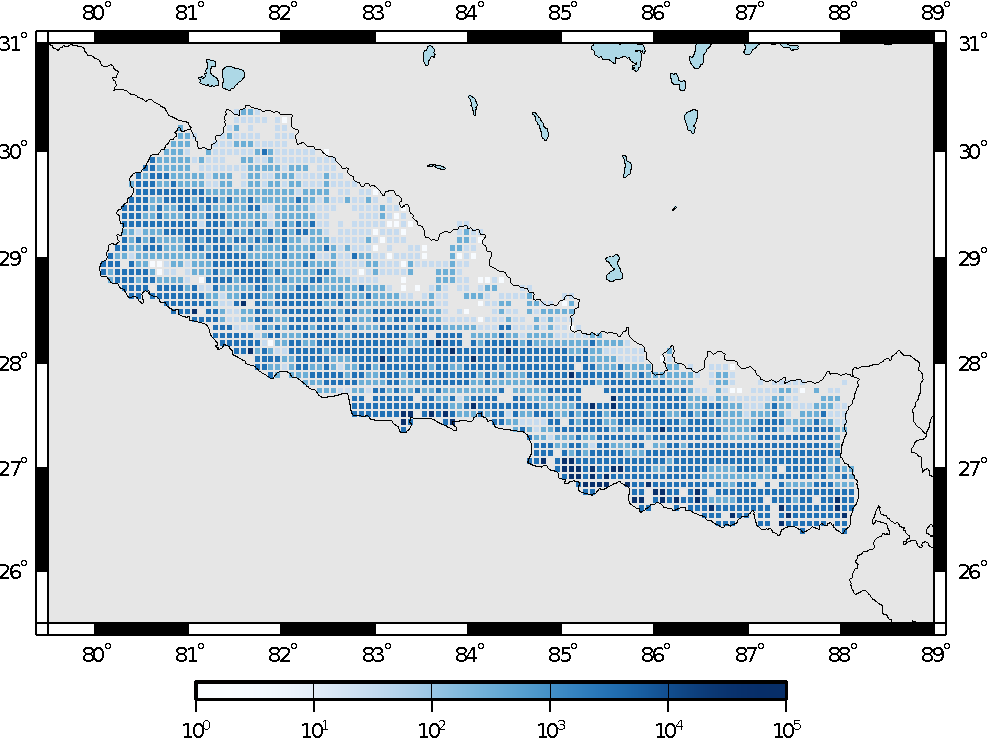
\includegraphics[width=12cm,height=8cm]{figures/risk/exposure-nepal.pdf}
\caption{Distribution of number of buildings in Nepal.}
\label{fig:exposure-nepal}
\end{figure}

The building portfolio was organised into four classes for the rural areas
(adobe, dressed stone, unreinforced fired brick, wooden frames), and five
classes for the urban areas (the aforementioned typologies, in addition to
reinforced concrete buildings). For each one of these building typologies,
\glspl{vulnerability function} and \glspl{fragility function} were collected
from the literature. These input models are only for demonstrative purposes
and for further information about the building characteristics of Nepal, users
are advised to contact the National Society for Earthquake Technology of Nepal
(NSET - \href{http://www.nset.org.np/}{http:www.nset.org.np/}).

The following sections include instructions not only on how to run the risk
calculations, but also on how to produce the necessary hazard inputs. Thus,
each demo comprises the configuration file, exposure model and fragility or
vulnerability models fundamental for the risk calculations. Each demo folder
also a configuration file and the input models to produce the relevant hazard
inputs.


\section{Scenario Damage Demos}
\label{sec:demos_scenario_damage}
A rupture of magnitude Mw 7 in the central part of Nepal is considered in this
demo. The characteristics of this rupture (geometry, dip, rake, hypocentre,
upper and lower seismogenic depth) are defined in the \verb+fault_rupture.xml+
file, and the hazard and risk calculation settings are specified in the
\verb+job.ini+ file.

To run the Scenario Damage demo, users should navigate to the folder where the
required files have been placed and employ following command:

\begin{minted}[fontsize=\footnotesize,frame=single,bgcolor=lightgray]{shell-session}
user@ubuntu:~\$ oq engine --run job_hazard.ini,job_risk.ini
\end{minted}

The hazard calculation should produce the following outputs:

\begin{minted}[fontsize=\footnotesize,frame=single,bgcolor=lightgray]{shell-session}
Calculation 8967 completed in 4 seconds. Results:
  id | output_type | name
9060 | datastore | gmfs
9061 | datastore | realizations
\end{minted}

and the following outputs should be produced by the risk calculation:

\begin{minted}[fontsize=\footnotesize,frame=single,bgcolor=lightgray]{shell-session}
Calculation 8968 completed in 16 seconds. Results:
  id | output_type | name
9062 | datastore | csq_by_asset
9063 | datastore | csq_by_taxon
9064 | datastore | csq_total
9065 | datastore | dmg_by_asset_and_collapse_map
9066 | datastore | dmg_by_taxon
9067 | datastore | dmg_total
\end{minted}


\section{Scenario Risk Demos}
\label{sec:demos_scenario_risk}
A rupture of magnitude 7 Mw in the central part of Nepal was considered within
this demo. The characteristics of this rupture (geometry, dip, rake,
hypocentre,  upper and lower seismogenic depth) have been defined in the
\verb+rupture.xml+ file, whist the hazard calculation settings have been
established on the \verb+job_hazard.ini+ file. In order to calculate the set of
ground motion fields due to this rupture, users should navigate to the folder
where the demo files are located, and use the following command:

\begin{Verbatim}[frame=single, commandchars=\\\{\}, samepage=true]
user@ubuntu:~\$ oq-engine --run job_hazard.ini
\end{Verbatim}

which will produce the following hazard result:

\begin{Verbatim}[frame=single, commandchars=\\\{\}, samepage=true]
Calculation 10 results:
id | output_type | name
20 | gmf_scenario | gmf_scenario
\end{Verbatim}

Then, this hazard input can be used for the risk calculations using the
following command:

\begin{Verbatim}[frame=single, commandchars=\\\{\}, samepage=true]
user@ubuntu:~\$ oq-engine --run job_risk.ini --hazard-output-id 20
\end{Verbatim}

leading to the following results:

\begin{Verbatim}[frame=single, commandchars=\\\{\}, samepage=true]
Calculation 11 results:
id | output_type | name
21 | aggregate_loss | Aggregate Loss type=structural
22 | loss_map | loss maps. type=structural
\end{Verbatim}

\section{Classical Probabilistic Seismic Damage Demos}
\label{sec:demos_classical_damage}
The seismic source model developed within the Global Seismic Hazard Assessment
Program (GSHAP) is used with the \cite{chiou2008} ground motion prediction
equation to produce the hazard input for this demo. No uncertainties are
considered in the seismic source model and since only one GMPE is being
considered, there will be only one possible path in the logic tree. Therefore,
only one set of seismic hazard curves will be produced. To run the hazard
calculation, the following command needs to be employed:

\begin{minted}[fontsize=\footnotesize,frame=single,bgcolor=lightgray]{shell-session}
user@ubuntu:~\$ oq engine --run job_hazard.ini
\end{minted}

which will produce the following sample hazard output:

\begin{minted}[fontsize=\footnotesize,frame=single,bgcolor=lightgray]{shell-session}
Calculation 8971 completed in 34 seconds. Results:
  id | name
9074 | hcurves
9075 | realizations
\end{minted}

The risk job calculates the probabilistic damage distribution for each asset
in the \gls{exposuremodel} starting from the above generated hazard curves. The
following command launches the risk calculations:

\begin{minted}[fontsize=\footnotesize,frame=single,bgcolor=lightgray]{shell-session}
user@ubuntu:~\$ oq engine --run job_risk.ini --hc 8971
\end{minted}

and the following sample outputs are obtained:

\begin{minted}[fontsize=\footnotesize,frame=single,bgcolor=lightgray]{shell-session}
Calculation 8972 completed in 16 seconds. Results:
  id | name
9076 | damages-rlzs
\end{minted}


\section{Classical Probabilistic Seismic Risk Demos}
\label{sec:demos_classical_risk}
The same hazard input as described in the Classical Probabilistic Damage demo
is used for this demo. Thus, the workflow to produce the set of hazard curves
described in Section~\ref{sec:demos_classical_damage} is also valid herein.
Then, to run the Classical Probabilistic Risk demo, users should navigate to
the folder containing the demo input models and configuration files and employ
the following command:

\begin{minted}[fontsize=\footnotesize,frame=single,bgcolor=lightgray]{shell-session}
user@ubuntu:~\$ oq engine --run job_hazard.ini
\end{minted}

which will produce the following hazard output:

\begin{minted}[fontsize=\footnotesize,frame=single,bgcolor=lightgray]{shell-session}
Calculation 8971 completed in 34 seconds. Results:
  id | output_type | name
9074 | datastore | hcurves
9075 | datastore | realizations
\end{minted}

In this demo, loss exceedance curves for each asset and two probabilistic loss
maps (for probabilities of exceedance of 1\% and 10\%) are produced. The
following command launches these risk calculations:

\begin{minted}[fontsize=\footnotesize,frame=single,bgcolor=lightgray]{shell-session}
user@ubuntu:~\$ oq engine --run job_risk.ini --hc 8971
\end{minted}

and the following outputs are expected:

\begin{minted}[fontsize=\footnotesize,frame=single,bgcolor=lightgray]{shell-session}
Calculation 8973 completed in 16 seconds. Results:
  id | output_type | name
9077 | datastore | loss_curves-rlzs
9078 | datastore | loss_maps-rlzs
\end{minted}


\section{Event Based Probabilistic Seismic Risk Demos}
\label{sec:demos_event_based_risk}
This demo uses the same probabilistic seismic hazard assessment (PSHA) model
described in the previous examples in Section~\ref{sec:demos_classical_damage}
and Section~\ref{sec:demos_classical_risk}. However, instead of hazard curves,
sets of ground motion fields will be generated by the hazard calculation of
this demo. Again, since there is only one branch in the logic tree, only one
set of ground motion fields will be used in the risk calculations. The hazard
and risk jobs are defined in a single configuration file for this demo. To
trigger the hazard and risk calculations the following command needs to be
used:

\begin{minted}[fontsize=\footnotesize,frame=single,bgcolor=lightgray]{shell-session}
user@ubuntu:~\$ oq engine --run job.ini
\end{minted}

and the following results are expected:

\begin{minted}[fontsize=\footnotesize,frame=single,bgcolor=lightgray]{shell-session}
Calculation 8974 completed in 229 seconds. Results:
  id | name
9079 | agg_curve-rlzs
9080 | agg_loss_table
9081 | loss_maps-rlzs
9082 | rcurves-rlzs
9083 | realizations
9084 | sescollection
\end{minted}


\section{Retrofit Benefit-Cost Ratio Demos}
\label{sec:demos_benefit_cost}
The loss exceedance curves used within this demo are produced using the
Classical Probabilistic Risk calculator. Thus, the process to produce the
seismic hazard curves described in Section~\ref{sec:demos_classical_risk} can
be employed here. Then, the risk calculations can be initiated using the
following command:

\begin{minted}[fontsize=\footnotesize,frame=single,bgcolor=lightgray]{shell-session}
user@ubuntu:~\$ oq engine --run job_risk.ini --hc 8971
\end{minted}

Alternatively, the hazard and risk jobs can be run sequentially using:

\begin{minted}[fontsize=\footnotesize,frame=single,bgcolor=lightgray]{shell-session}
user@ubuntu:~\$ oq engine --run job_hazard.ini,job_risk.ini
\end{minted}

which should produce the following output:

\begin{minted}[fontsize=\footnotesize,frame=single,bgcolor=lightgray]{shell-session}
Calculation 8976 completed in 14 seconds. Results:
  id | output_type | name
9087 | datastore | bcr-rlzs
\end{minted}

   \cleardoublepage

% -------------------------------------------------------- Part IV: Appendices -
%\thispagestyle{empty}
%\part*{Appendices}
%\appendix
%
%\chapterimage{figures/chapter_head_2.pdf} % Chapter heading image
%\chapter{Ground Shaking Intensity Models}
%   \label{chap:gsims}
%	We provide below a list of the ground motion prediction equations implemented
in the \gls{acr:hazlib}. All the implemented \gls{acr:gmpe} use moment
magnitude as the reference magnitude. For each GMPE, the \gls{acr:oqe} name, a
short description, and the corresponding reference are given.


\section[GMPEs for shallow earthquakes in active tectonic regions]{Ground motion prediction equations for shallow earthquakes in active tectonic regions}

\begin{itemize}

\item AbrahamsonSilva2008 \hfill \\ A ground motion prediction equation
developed in the context of the NGA West project \footnote{\href{http://peer.
berkeley.edu/ngawest/}{http://peer.berkeley.edu/ngawest}}. The model is
applicable to magnitudes 5.0-8.5, distances 0-200 km, and spectral periods 0-10
sec (\cite{abrahamson2008}).

\item AkkarBommer2010 \hfill \\ A ground motion prediction equation developed
using mostly data from Europe and the Middle East. The dataset used to derive
these equations contains events with moment magnitude between 5.0 and 7.6 and
distances up to 100 km (\cite{akkar2010}).

\item AkkarCagnan2010 \hfill \\ A ground motion prediction equation for
shallow earthquakes in active tectonic regions developed using data from the
Turkish strong-motion database. Equations are valid for a distance range of
0–200 km and are derived for moment magnitudes between 5.0 and 7.6
(\cite{akkar2010a}).

\item BooreAtkinson2008 \hfill \\ A ground motion prediction equation for
shallow earthquakes in active tectonic regions developed in the context of the
NGA West project. The model is applicable to magnitude in the range 5.0-8.0,
distances $<$ 200 km, and spectral periods 0-10 (\cite{boore2008}).

\item CauzziFaccioli2008 \hfill \\ A ground motion prediction equation derived
from global data base of shallow crustal earthquakes (vast majority coming
from Japan) with magnitudes in range 5-7.2 and distances $<$ 150.0
(\cite{cauzzi2008}).

\item ChiouYoungs2008 \hfill \\ A ground motion prediction equation for
shallow earthquakes in active tectonic regions developed in the context of the
NGA West \footnote{
\href{http://peer.berkeley.edu/ngawest/}{http://peer.berkeley.edu/ngawest}}.
The model is supposed to be applicable for magnitude in range 4.0-8.5 (if
strike-slip), 4.0-8.0 (if normal or reverse) and distances 0-200 km.

\item FaccioliEtAl2010 \hfill \\ Based on the same functional form of
\cite{cauzzi2008} but using closest distance to the rupture instead of
hypocentral distance (\cite{faccioli2010})

\item SadighEtAl1997 \hfill \\ A ground motion prediction based primarily on
strong motion data from California and applicable for magnitude in range 4.0-8.0
and distances $<$ 100 km (\cite{sadigh1997}).

\item ZhaoEtAl2006Asc \hfill \\ A ground motion prediction equation for active
shallow crust events developed using mostly japanese strong ground motion
recordings (\cite{zhao2006}).

\end{itemize}



\section[GMPEs for subduction sources]{Ground motion prediction equations for subduction sources}

\begin{itemize}

\item AtkinsonBoore2003SInter, AtkinsonBoore2003SSlab \hfill \\ Ground motion
prediction equations for subduction interface and in-slab events obtained
using a global dataset of subduction earthquakes with moment magnitude between
5.0 and 8.3 (\cite{atkinson2003}).

\item LinLee2008SInter, LinLee2008SSlab \hfill \\ Ground motion prediction
equations for subduction interface and in-slab events created using strong
motion data included in the the Taiwanese database (\cite{lin2008}).

\item YoungsEtAl1997SInter, YoungsEtAl1997SSlab \hfill \\ One of the most well
known ground motion prediction equations for subduction earthquakes. Published
in 1997, is still currently used for the calculation of the ground motion in
subduction tectonic environments. This GMPE covers events of moment magnitude
greater than 5.0 occurred at a distance between 5 and 500 km. The source-site
distance metric is the \gls{acr:rrup}. (\cite{youngs1997})

\item ZhaoEtAl2006SInter, ZhaoEtAl2006SSlab \hfill \\ Ground motion
prediction equations for subduction interface and in-slab developed
using mostly japanese strong ground motion recordings (\cite{zhao2006}).

\end{itemize}



\section[GMPEs for stable continental regions]{Ground motion prediction equations for stable continental regions}

\begin{itemize}

\item AtkinsonBoore2006 \hfill \\ A ground motion prediction equation for
Eastern North America derived from a stochastic finite fault model
(\cite{atkinson2006}).

\item Campbell2003 \hfill \\ Ground motion prediction equation calibrated for
Eastern North America applicable for events with magnitude greater than 5.0 and
distances $<$ 70 km (\cite{campbell2003}).

\item ToroEtAl2002 \hfill \\ Ground motion prediction equation for rock sites
in central and eastern North America based on the prediction of a stochastic
ground-motion model. The model is applicable for magnitudes in range 5.0-8.0 and
distances in 1-500 km (\cite{toro2002}).

\end{itemize}

%   \cleardoublepage


%-------------------------------------------------------------------------------
%  BIBLIOGRAPHY
%-------------------------------------------------------------------------------

\chapter*{Bibliography}
\addcontentsline{toc}{chapter}{\textcolor{darkgray}{Bibliography}}
\section*{Books}
\printbibliography[heading=bibempty,type=book]
\section*{Articles}
\printbibliography[heading=bibempty,type=article]
\section*{Other Sources}
\printbibliography[heading=bibempty,nottype=book,nottype=article]
\cleardoublepage

%-------------------------------------------------------------------------------
%  INDEX & GLOSSARY
%-------------------------------------------------------------------------------

\printindex
\chapter*{Glossary}
\addcontentsline{toc}{chapter}{\textcolor{darkgray}{Glossary}}
\printglossary[type=acronym, title=List of Acronyms]
\printglossary[title=List of Terms]
\hfill \\ \thispagestyle{empty} \clearpage % ---------------- Final empty page -

\end{document}
